\documentclass[a4paper,12pt, titlepage]{report}
\usepackage{polski}
\usepackage[polish]{babel}
\usepackage[utf8]{inputenc}
\usepackage{placeins}
\usepackage{graphicx}

%%% PACKAGES
\usepackage{subfig} % make it possible to include more than one captioned figure/table in a single float

\usepackage{hyperref}
\hypersetup{
	colorlinks=true,
	linkcolor=blue,
	filecolor=magenta,      
	urlcolor=cyan,
}

\usepackage[a4paper,width=150mm,top=20mm,bottom=20mm]{geometry}
\usepackage{lmodern}  % for bold teletype font
\usepackage{amsmath}  % for \hookrightarrow
\usepackage{xcolor}   % for \textcolor

% for Python listings
\usepackage{listings}
\lstset{
  basicstyle=\ttfamily,
  columns=fullflexible,
  frame=single,
  breaklines=true,
  postbreak=\mbox{\textcolor{red}{$\hookrightarrow$}\space},
}
\usepackage{titlesec}
\newcommand{\sectionbreak}{\clearpage}
\usepackage[nottoc,notlof,notlot]{tocbibind}
\usepackage[titles,subfigure]{tocloft}
\renewcommand{\cftsecfont}{\rmfamily\mdseries\upshape}
\renewcommand{\cftsecpagefont}{\rmfamily\mdseries\upshape}

\graphicspath{ {./images/} }

\def\uczelnia{{Uniwersytet Kardynała Stefana Wyszyńskiego w~Warszawie}\\
Wydział Matematyczno-Przyrodniczy \\ Szkoła Nauk Ścisłych}
\def\nralbumu{107418}
\title{Wprowadzenie do Przetwarzanie obrazów\\Sprawozdanie z laboratorium}
\author{Małgorzata Wiśniewska\\107418}
\date{Warszawa, 2020} 

\begin{document}
\maketitle
\tableofcontents
\chapter{Wstęp}
\section{Format obrazów}
\par Portable Network Graphics (PNG) jest formatem pliku komputerowego do przechowywania obrazów grafiki rastrowej, stworzony jako odpowiedź na roszczenia patentowe dotyczące kompresji LZW, wykorzystywanej w formatach GIF i TIFF. \\\\PNG jest jedynym wieloplatformowym formatem bitmapowym, umożliwiającym zdefiniowanie stopnia przezroczystości (kanał \(\alpha\)). Obsługuje 48-bitową głębię kolorów czyli 16 bitów na kanał koloru. Dzięki tym dwóm cechom możliwe jest praktycznie bezstratne zapisanie dowolnej grafiki RGB oraz RGBA. Obsługuje także osadzone profile kolorów ICC, ICM i dane EXIF. Format PNG zapisuje tylko pojedyncze pliki graficzne - nie ma animacji.
\subsection*{Struktura pliku PNG}
\par Plik PNG podzielony jest na dwie części:
\begin{enumerate}
\item nagłówek pliku obrazowego
\begin{itemize}
\item zaczyna się 8 bajtowych podpisem
\item \textbf{89} - wysoki bit ustawiony w celu rozpoznania systemów, które nie wspierają 8 bitowych danych i odróżnienia plików tekstowych od plików PNG
\item \textbf{50 4E 47} - kod ASCII odpowiadający literom PNG pozwala na rozpoznanie pliku PNG ludziom
\item \textbf{0D 0A} - znak końca linii w stylu DOS, aby rozpoznać DOSowo-Unixowe zakończenia linii w konwersji danych
\item \textbf{1A} - bit kończący plik w DOS
\item \textbf{0A} - bit kończący plik w Unix
\end{itemize}
\item katalog pliku obrazowego
\begin{itemize}
\item składa się z kawałków (ang. \textit{chunks})
\item każdy kawałek składa się z czterech części: długości (4 bajty), typu kawałka (4 bajty), danych (tyle bajtów ile zadeklarowano w długości) oraz sumy kontrolnej (4 bajty, ang. \textit{CRC, checksum})
\item najważniejsze, krytyczne dla poprawnego działania kawałki:
\begin{itemize}
\item \textbf{IHDR} - zawiera informacje o szerokośći, wysokości, głębokości, barwie, metodzie kompresji, metodzie filtracji i metodzie przeplotu w obrazie.
\item \textbf{PLTE} - zawiera listę kolorów
\item \textbf{IDAT} - zawiera obraz, który może być podzielony między wiele kawałków IDAT
\item \textbf{IEND} - oznacza koniec obrazu
\end{itemize}
\end{itemize}
\end{enumerate}
\subsection*{Przykładowa struktura prostego pliku PNG}
\begin{figure}[h]
    \centering
    \subfloat{{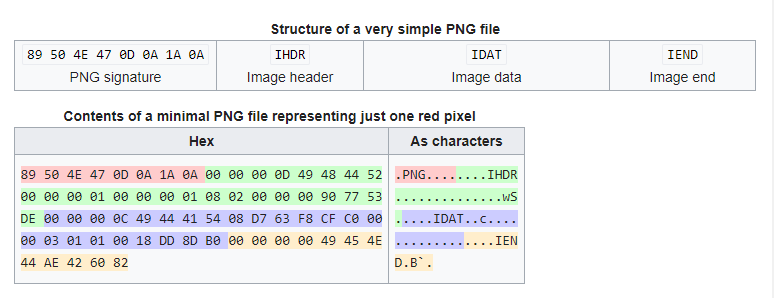
\includegraphics[width=1\textwidth]{./examplePNG.png} }}%
    \caption{Przykładowa struktura pliku PNG [żródło: wikipedia.org]}%
    \label{fig:geo_before_grey1}%
\end{figure}
\FloatBarrier
\section{Instrukcja obsługi programu}
Implementacja zadań została napisana w języku Python3. Wykorzystane biblioteki to numpy, matplotlib oraz Pillow. Przykład instalacji biblioteki: \\\\ \textbf{\textit{pip install}} numpy\\ \textbf{\textit{pip install}} matplotlib\\ \textbf{\textit{pip install}} pillow\\\\Aby wystartować program i rozpocząć otrzymywanie wyników przetwarzania pozczególnych obrazów należy uruchomić plik app.py Przykład uruchomienia programu: \\\\ \textbf{\textit{python}} app.py

\chapter{Operacje ujednolicania obrazów}
Operacje ujednolicania obrazów dzieli się na dwa etapy. Pierwszym etapem jest ujednolicanie geometryczne, drugim jest ujednolicenie rozdzielczościowe. W prezentowanym programie ujednolicane są dwa obrazy, w taki sposób, że mniejszy z nich jest doprowadzany do takiego samego rozmiaru jak większy. Skutkuje to wygenerowaniem nowego obrazu o zwiększonej ilości piksli niż początkowa wartość. Dzięki zastosowaniu tego typu ujednolicania w efekcie nie następuje widoczny spadek jakości. 

\section{Ujednolicanie obrazów szarych geometryczne}
\subsection*{Opis algorytmu}
\par Operacje geometrycznego ujednolicania polega na wyrównaniu liczby piksli w kolumnach i wierszach w obu obrazach, poprzez zwiększenie liczby piksli w kolumnach i wierszach mniejszego z obrazów.
\begin{enumerate}
\item Wybierz największą wysokość i największą szerokość spośród obu obrazów.
\item Jeśli dany obraz ma mniejszą wysokość lub szerokość, wypełnij różnicę pikslami o wartości 1, tak, żeby wysokość i szerokość obu obrazów była równa.
\end{enumerate}
\subsection*{Efekty wykorzystania algorytmu}
\begin{figure}[h]
    \centering
    \subfloat[Obraz 1: 256x256]{{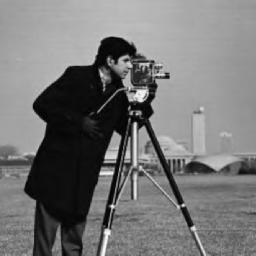
\includegraphics[width=0.4\textwidth]{./RawPictures/fotograf.png} }}%
    \qquad
    \subfloat[Obraz 2: 512x512]{{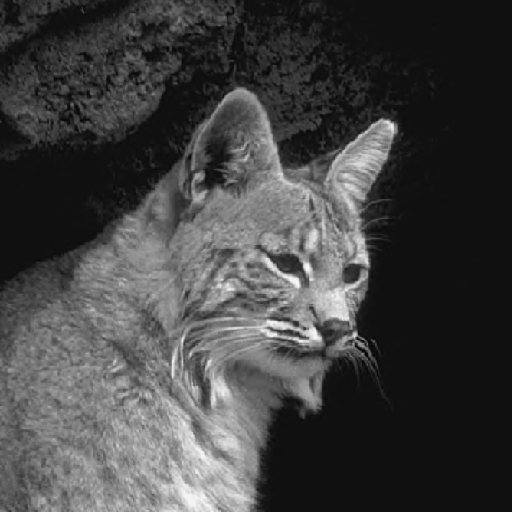
\includegraphics[width=0.4\textwidth]{./RawPictures/rys.png} }}%
    \caption{Obrazy wejściowe}%
    \label{fig:geo_before_grey1}%
\end{figure}
\FloatBarrier
\begin{figure}[h]
    \centering
    \subfloat[Obraz 1: 512x512]{{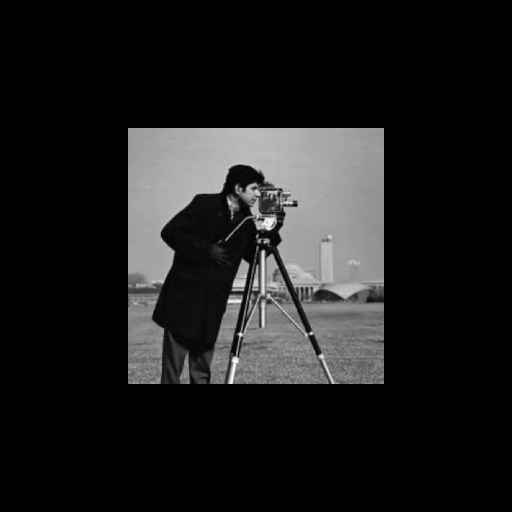
\includegraphics[width=0.4\textwidth]{./ExEffects/1/11/fotograf_rys.png} }}%
    \qquad
    \subfloat[Obraz 2: 512x512]{{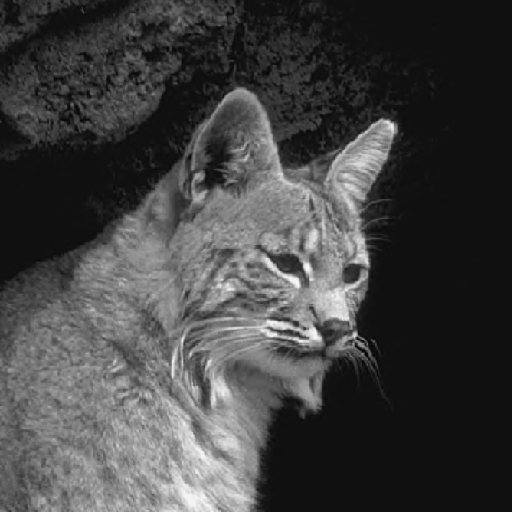
\includegraphics[width=0.4\textwidth]{./RawPictures/rys.png} }}%
    \caption{Obrazy wyjściowe}%
    \label{fig:geo_after_grey1}%
\end{figure}
\FloatBarrier
\begin{figure}[h]
    \centering
    \subfloat[Obraz 1: 369x480]{{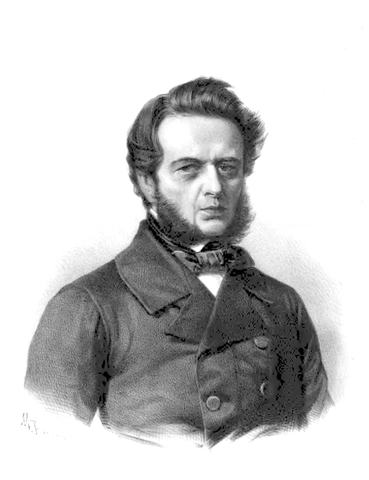
\includegraphics[width=0.4\textwidth]{./RawPictures/AndrzejZamoyski.png} }}%
    \qquad
    \subfloat[Obraz 2: 623x640]{{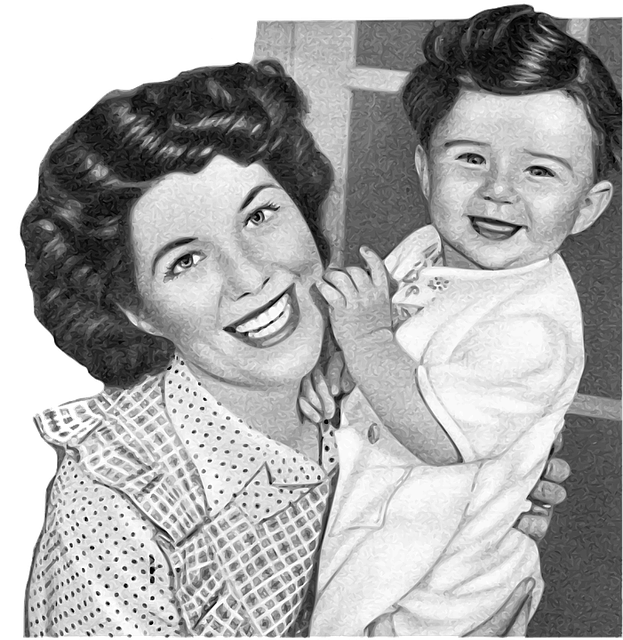
\includegraphics[width=0.4\textwidth]{./RawPictures/kobietaDziecko.png} }}%
    \caption{Obrazy wejściowe}%
    \label{fig:geo_before_grey2}%
\end{figure}
\FloatBarrier
\begin{figure}[h]
    \centering
    \subfloat[Obraz 1:  623x640]{{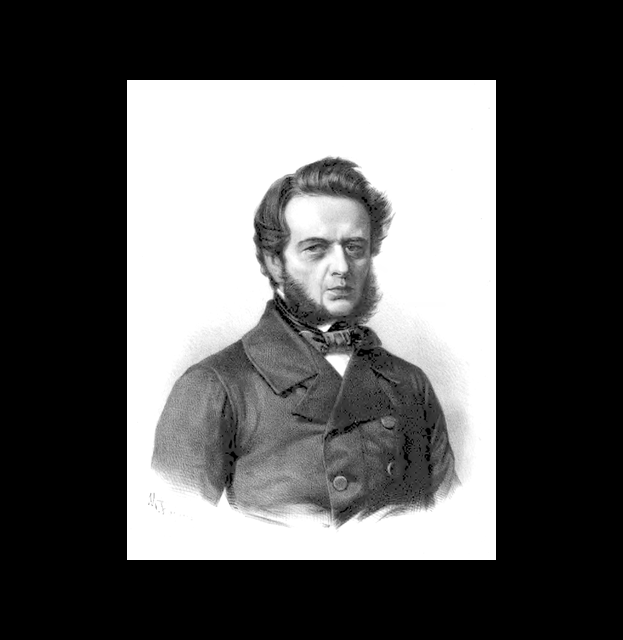
\includegraphics[width=0.4\textwidth]{./ExEffects/1/11/AndrzejZamoyski_kobietaDziecko.png} }}%
    \qquad
    \subfloat[Obraz 2:  623x640]{{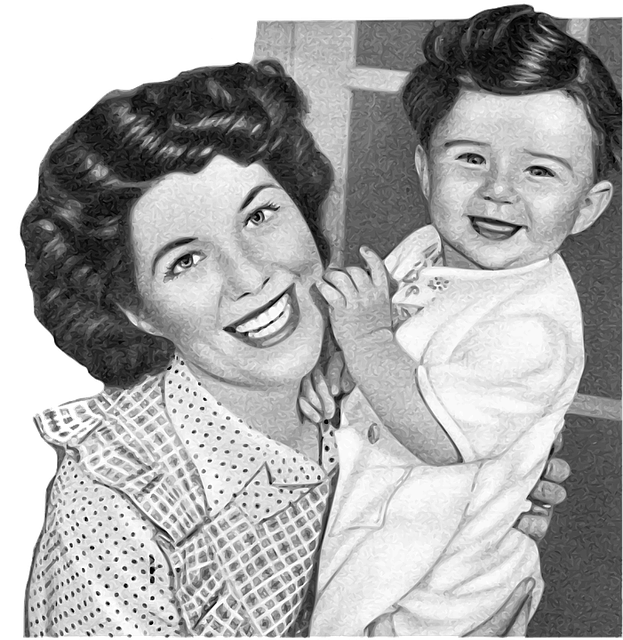
\includegraphics[width=0.4\textwidth]{./RawPictures/kobietaDziecko.png} }}%
    \caption{Obrazy wyjściowe}%
    \label{fig:geo_after_grey2}%
\end{figure}
\FloatBarrier
\subsection*{Kod źródłowy algorytmu}
\begin{lstlisting}[language=Python]
def geoUnificationGrey(self):
	# porownaj wielkosc obrazow, jezeli sa tego samego rozmiaru nie rob nic
	if self.biggerPicture == 0 and self.smallerPicture == 0:
		print('Both pictures have the same size')
		return 0
	# stworz tablice zer do zapisu efektu algorytmu
	result = np.zeros((self.maxLength, self.maxWidth), np.uint8)
	startWidthIndex = int(round((self.maxWidth - self.minWidth) / 2))
	startLengthIndex = int(round((self.maxLength - self.minLength) / 2))
	for w in range(0, self.minWidth):
		for l in range(0, self.minLength):
			result[l + startLengthIndex, w + startWidthIndex] = self.matrix[l, w]
	#zapisz zunifikowany obraz
	path = self.ex + self.smallerPictureName + '_' + self.biggerPictureName + '.png'
	self.saver.savePictureFromArray(result, 'L', path)
\end{lstlisting}

\section{Ujednolicanie obrazów szarych rozdzielczościowe}
\subsection*{Opis algorytmu}
\par Operacja rozdzielczościowego ujednolicania obrazów następuje po ujednoliceniu geometrycznym obrazów wejściowych. Polega na wypełnieniu obrazu pikslami. Brakujące piksle powinny zostać zinterpolowane.
\begin{enumerate}
\item Wypełnij cały obraz pikslami o znanej wartości zachowując pewien odstęp między nimi, gdzie odstępem będą piksle o wartości 0.
\item Każdemu pikslowi o nieznanej wartości przypisz średnią wartość znanych (>0) piksli z jego bezpośredniego otoczenia.
\end{enumerate}
\subsection*{Efekty wykorzystania algorytmu}
\begin{figure}[h]
    \centering
    \subfloat[Obraz 1: 512x512]{{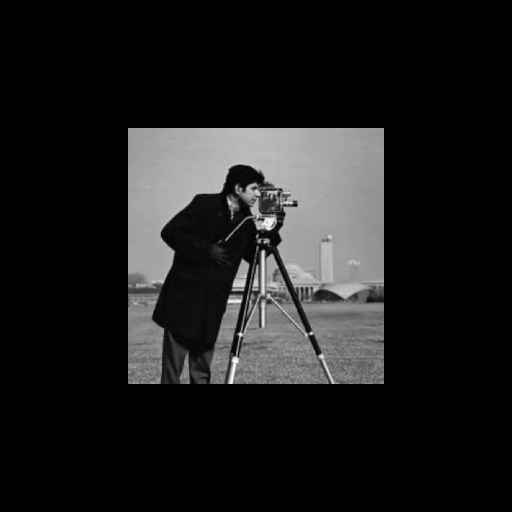
\includegraphics[width=0.4\textwidth]{./ExEffects/1/11/fotograf_rys.png} }}%
    \qquad
    \subfloat[Obraz 2: 512x512]{{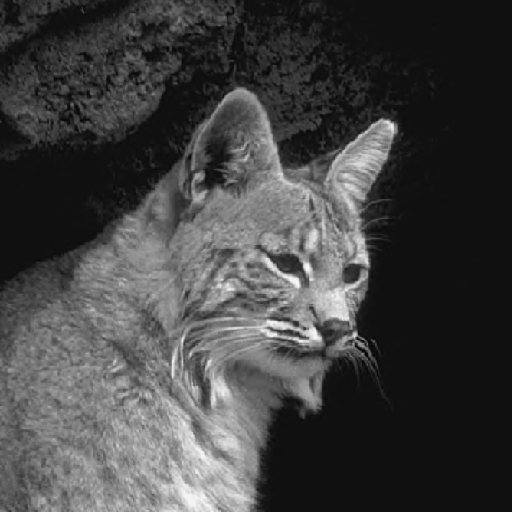
\includegraphics[width=0.4\textwidth]{./RawPictures/rys.png} }}%
    \caption{Obrazy wejściowe po ujednoliceniu geometrycznym}%
    \label{fig:example}%
\end{figure}
\FloatBarrier
\begin{figure}[h]
    \centering
    \subfloat[Obraz 1: 512x512]{{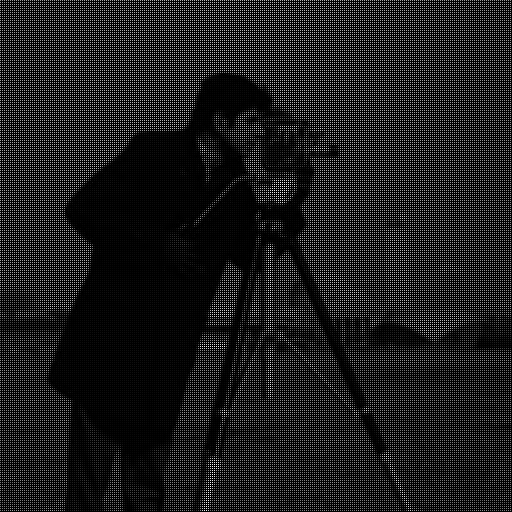
\includegraphics[width=0.4\textwidth]{./ExEffects/1/12/fotograf_rys_withoutInterpolation.png} }}%
    \qquad
    \subfloat[Obraz 2: 512x512]{{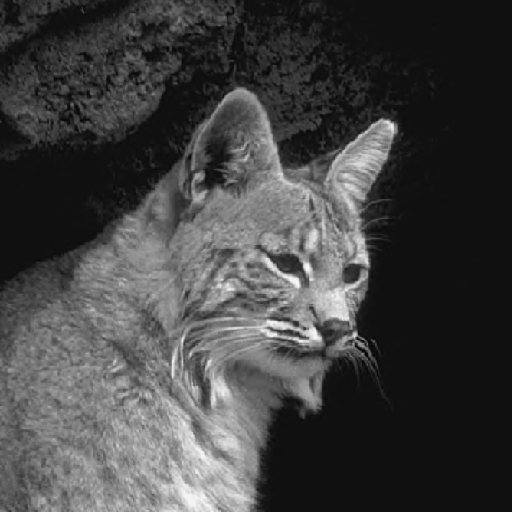
\includegraphics[width=0.4\textwidth]{./RawPictures/rys.png} }}%
    \caption{Obrazy wyjściowe bez interpolacji}%
    \label{fig:example}%
\end{figure}
\FloatBarrier
\begin{figure}[h]
    \centering
    \subfloat[Obraz 1: 512x512]{{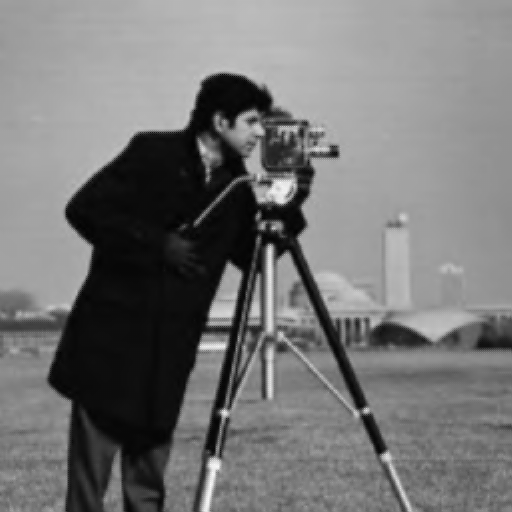
\includegraphics[width=0.4\textwidth]{./ExEffects/1/12/fotograf_rys_withInterpolation.png} }}%
    \qquad
    \subfloat[Obraz 2: 512x512]{{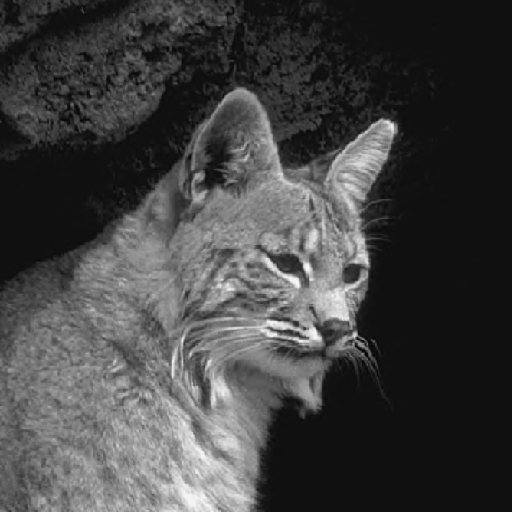
\includegraphics[width=0.4\textwidth]{./RawPictures/rys.png} }}%
    \caption{Obrazy wyjściowe po interpolacji}%
    \label{fig:example}%
\end{figure}
\FloatBarrier
\subsection*{Kod źródłowy algorytmu}
\begin{lstlisting}[language=Python]
def resolutionUnificationGrey(self):
    print('Beginning of resolution unification for two grey pictures.')
    if self.biggerPicture == 0 and self.smallerPicture == 0:
        print('Both pictures have the same size')
        return 0
    scaleFactorLength = float(self.maxLength / self.minLength)
    scaleFactorWidth = float(self.maxWidth / self.minWidth)
    result = np.zeros((self.maxLength, self.maxWidth), np.uint8)
    for l in range(self.minLength):
        for w in range(self.minWidth):
            if w % 2 == 0:
                pomL = int(scaleFactorLength * l)
                pomW = int(round(scaleFactorWidth * w))
                result[pomL, pomW] = self.matrix[l, w]
            elif w % 2 == 1:
                pomL = int(round(scaleFactorLength * l))
                pomW = int(scaleFactorWidth * w)
                result[pomL, pomW] = self.matrix[l, w]
    # zapisz obraz bez interpolacji
    path = self.ex + self.smallerPictureName + '_' + self.biggerPictureName + '_withoutInterpolation.png'
    self.saver.savePictureFromArray(result, 'L', path)
    # interpolacja
    for l in range(self.maxLength):
        for w in range(self.maxWidth):
            value = 0
            count = 0
            if result[l, w] == 0:
                for lOff in range(-1, 2):
                    for wOff in range(-1, 2):
                        lSave = l if ((l + lOff) > (self.maxLength - 2)) | ((l + lOff) < 0) else (l + lOff)
                        wSave = w if ((w + wOff) > (self.maxWidth - 2)) | ((w + wOff) < 0) else (w + wOff)
                        if result[lSave, wSave] != 0:
                            value += result[lSave, wSave]
                            count += 1
                result[l, w] = value / count
    # zapisz obraz po interpolacji
    path = self.ex + self.smallerPictureName + '_' + self.biggerPictureName + '_withInterpolation.png'
    self.saver.savePictureFromArray(result, 'L', path)
    print('Finished resolution unification.')
\end{lstlisting}

\section{Ujednolicanie obrazów RGB geometryczne}
\subsection*{Opis algorytmu}
\par Operacje geometrycznego ujednolicania polega na wyrównaniu liczby piksli w kolumnach i wierszach w obu obrazach, poprzez zwiększenie liczby piksli w kolumnach i wierszach mniejszego z obrazów.
\begin{enumerate}
\item Wybierz największą wysokość i największą szerokość spośród obu obrazów.
\item Jeśli dany obraz ma mniejszą wysokość lub szerokość, wypełnij różnicę pikslami o wartości 1 dla każdego z kanałów (R,G,B), tak, żeby wysokość i szerokość obu obrazów była równa.
\end{enumerate}
\subsection*{Efekty wykorzystania algorytmu}
\begin{figure}[h]
    \centering
    \subfloat[Obraz 1: 512x512]{{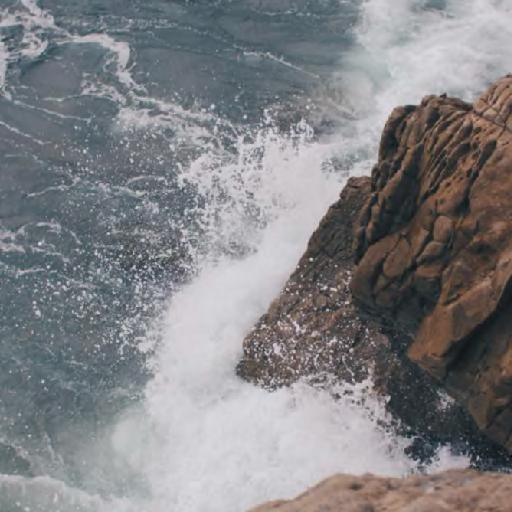
\includegraphics[width=0.4\textwidth]{./RawPictures/morze.png} }}%
    \qquad
    \subfloat[Obraz 2: 1025x1025]{{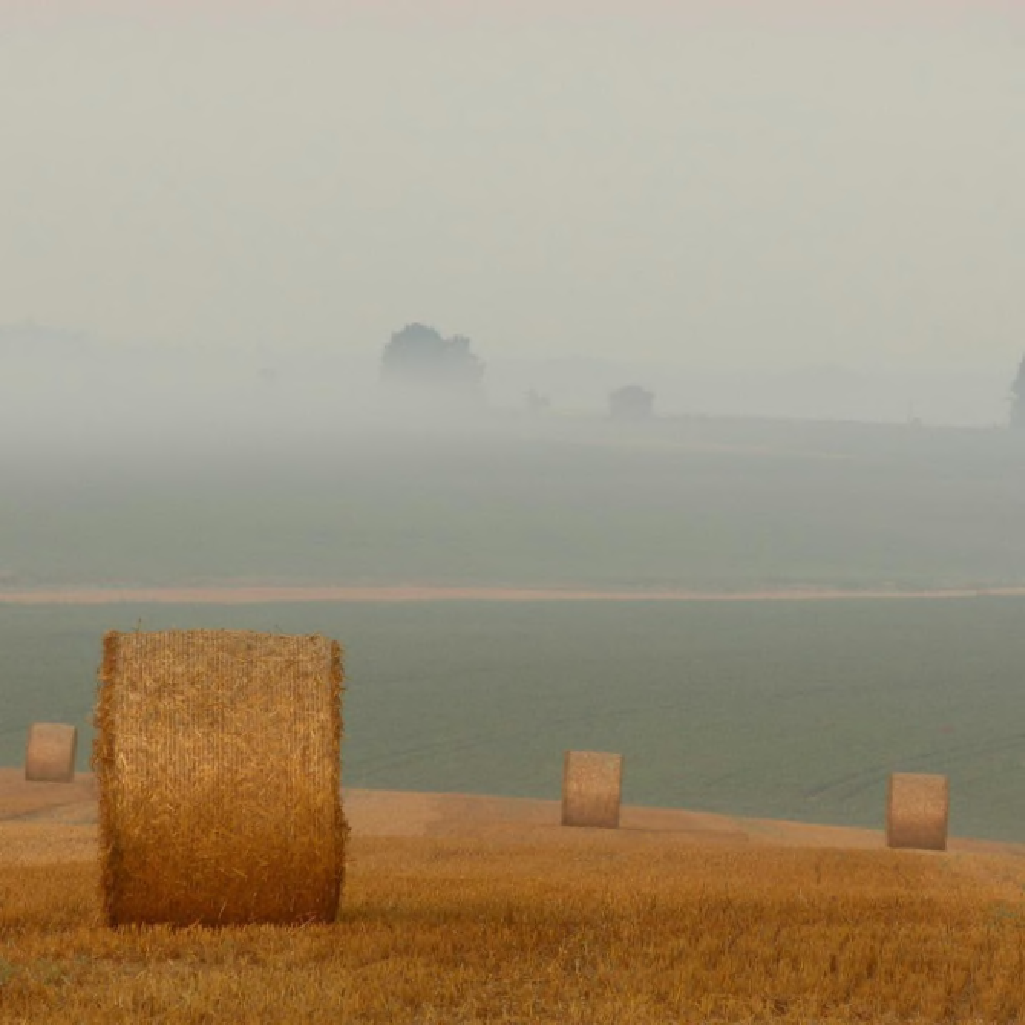
\includegraphics[width=0.4\textwidth]{./RawPictures/stogi.png} }}%
    \caption{Obrazy wejściowe}%
    \label{fig:geo_before_grey1}%
\end{figure}
\FloatBarrier
\begin{figure}[h]
    \centering
    \subfloat[Obraz 1: 1025x1025]{{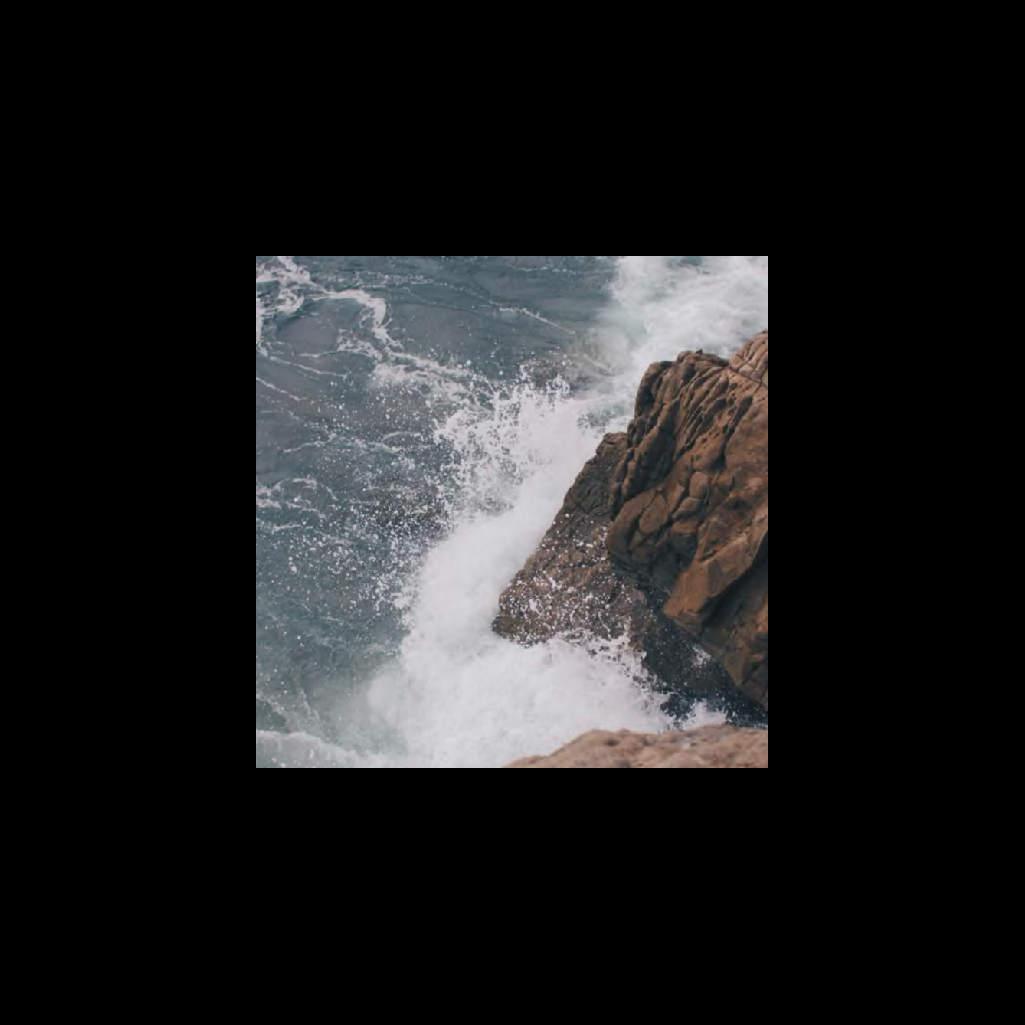
\includegraphics[width=0.4\textwidth]{./ExEffects/1/13/morze_stogi.png} }}%
    \qquad
    \subfloat[Obraz 2: 1025x1025]{{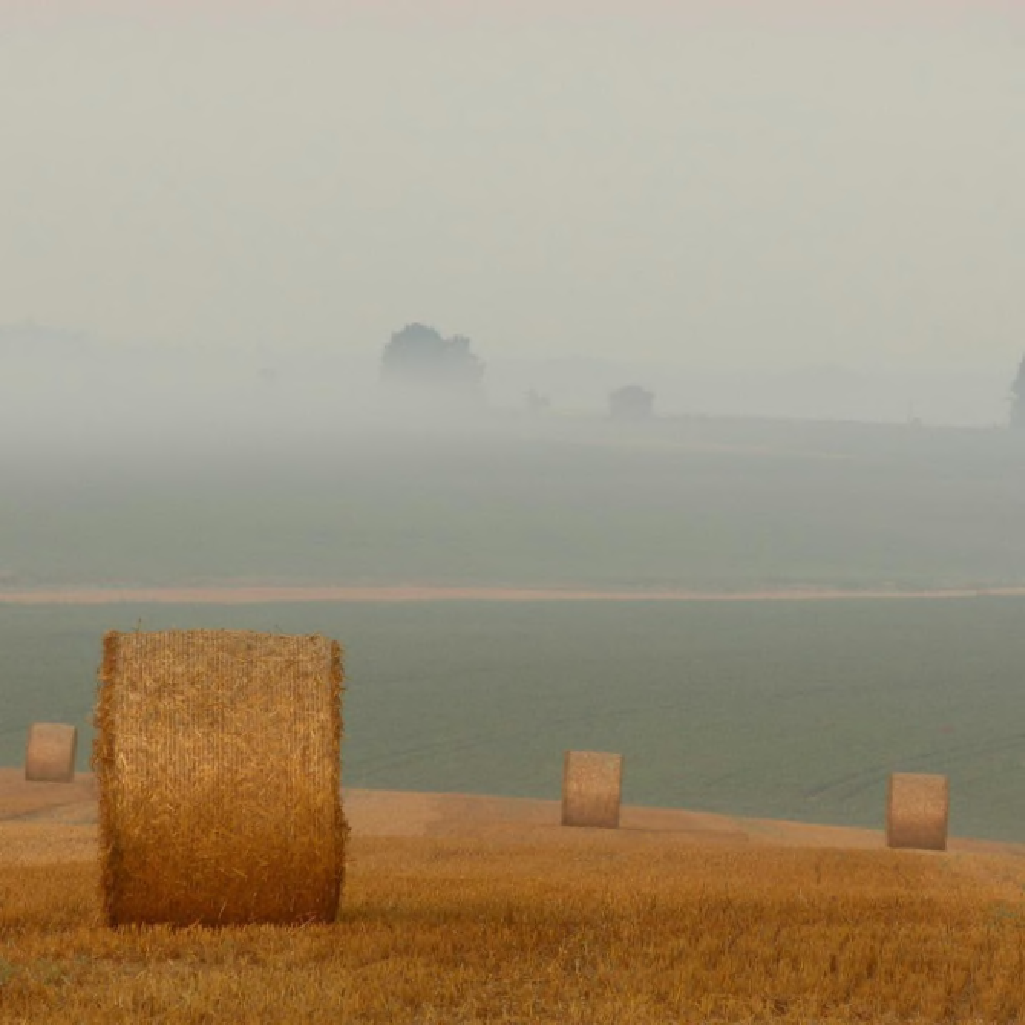
\includegraphics[width=0.4\textwidth]{./RawPictures/stogi.png} }}%
    \caption{Obrazy wyjściowe}%
    \label{fig:geo_after_grey1}%
\end{figure}
\FloatBarrier
\begin{figure}[h]
    \centering
    \subfloat[Obraz 1: 256x256]{{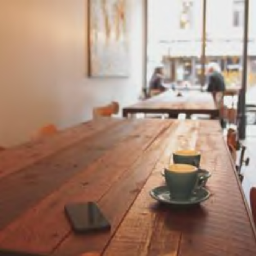
\includegraphics[width=0.4\textwidth]{./RawPictures/kawa.png} }}%
    \qquad
    \subfloat[Obraz 2: 512x512]{{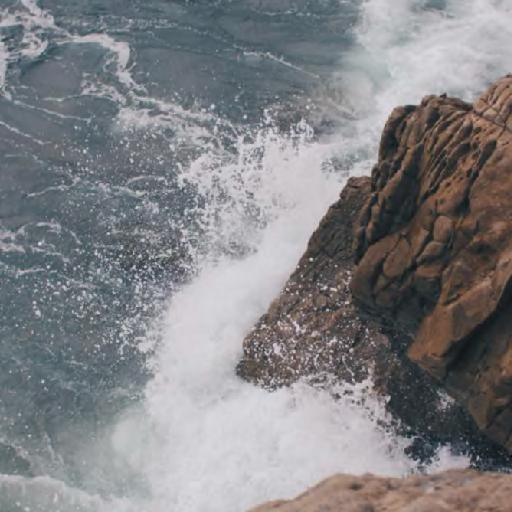
\includegraphics[width=0.4\textwidth]{./RawPictures/morze.png} }}%
    \caption{Obrazy wejściowe}%
    \label{fig:geo_before_grey2}%
\end{figure}
\FloatBarrier
\begin{figure}[h]
    \centering
    \subfloat[Obraz 1:  512x512]{{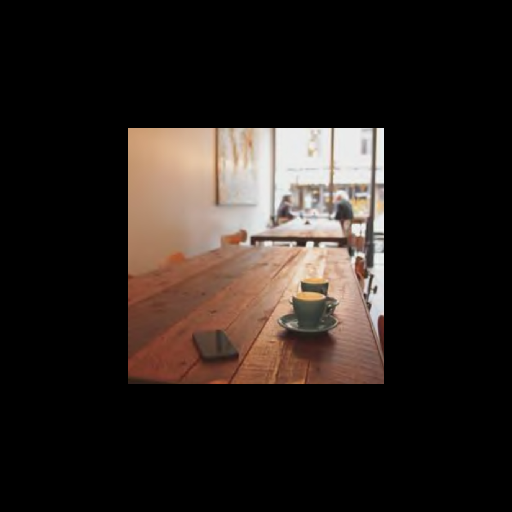
\includegraphics[width=0.4\textwidth]{./ExEffects/1/13/kawa_morze.png} }}%
    \qquad
    \subfloat[Obraz 2:  512x512]{{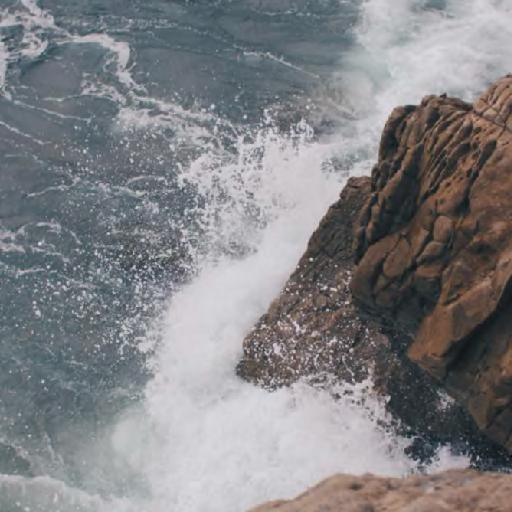
\includegraphics[width=0.4\textwidth]{./RawPictures/morze.png} }}%
    \caption{Obrazy wyjściowe}%
    \label{fig:geo_after_grey2}%
\end{figure}
\FloatBarrier
\subsection*{Kod źródłowy algorytmu}
\begin{lstlisting}[language=Python]
def geoUnificationRGB(self):
    if self.biggerPicture == 0 and self.smallerPicture == 0:
        print('Both pictures have the same size')
        return 0
    # stworz tablice z zerami jako odstawe dla unifikacji
    result = np.full((self.maxLength, self.maxWidth, 3), 0, np.uint8)
    startWidthIndex = int(round((self.maxWidth - self.minWidth) / 2))
    startLengthIndex = int(round((self.maxLength - self.minLength) / 2))
    for w in range(0, self.minWidth):
        for l in range(0, self.minLength):
            result[l + startLengthIndex, w + startWidthIndex] = self.matrix[w, l]
    # zapisz zunifikowany obraz
    path = self.ex + self.smallerPictureName + '_' + self.biggerPictureName + '.png'
    self.saver.savePictureFromArray(result, 'RGB', path)
\end{lstlisting}

\section{Ujednolicanie obrazów RGB rozdzielczościowe}
\subsection*{Opis algorytmu}
\par Operacja rozdzielczościowego ujednolicania obrazów następuje po ujednoliceniu geometrycznym obrazów wejściowych. Polega na wypełnieniu obrazu pikslami. Brakujące piksle powinny zostać zinterpolowane.
\begin{enumerate}
\item Wypełnij cały obraz pikslami o znanej wartości zachowując pewien odstęp między nimi, gdzie odstępem będą piksle o wartości 0.
\item Każdemu pikslowi (ze wszystkich kanałów - R, G, B) o nieznanej wartości przypisz średnią wartość znanych (>0) piksli z jego bezpośredniego otoczenia.
\end{enumerate}
\subsection*{Efekty wykorzystania algorytmu}
\begin{figure}[h]
    \centering
    \subfloat[Obraz 1: 1025x1025]{{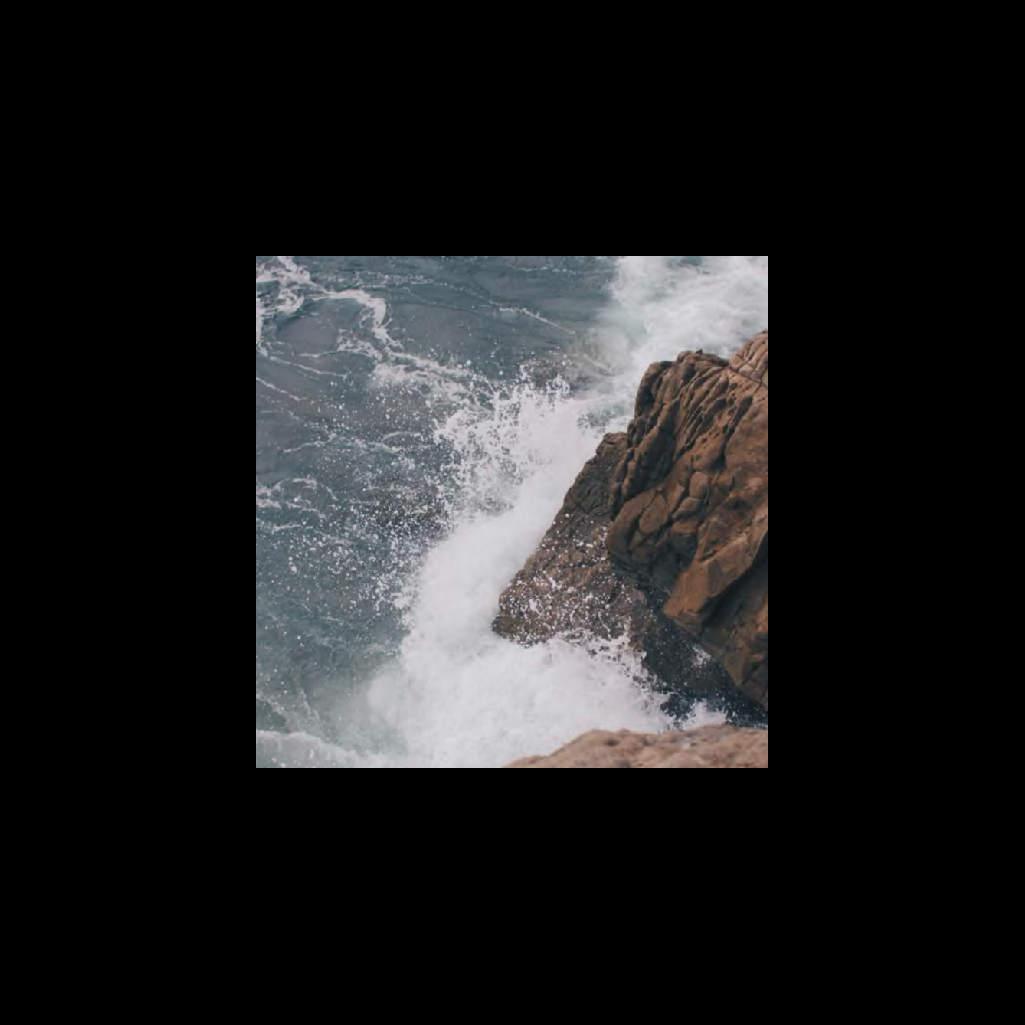
\includegraphics[width=0.4\textwidth]{./ExEffects/1/13/morze_stogi.png} }}%
    \qquad
    \subfloat[Obraz 2: 1025x1025]{{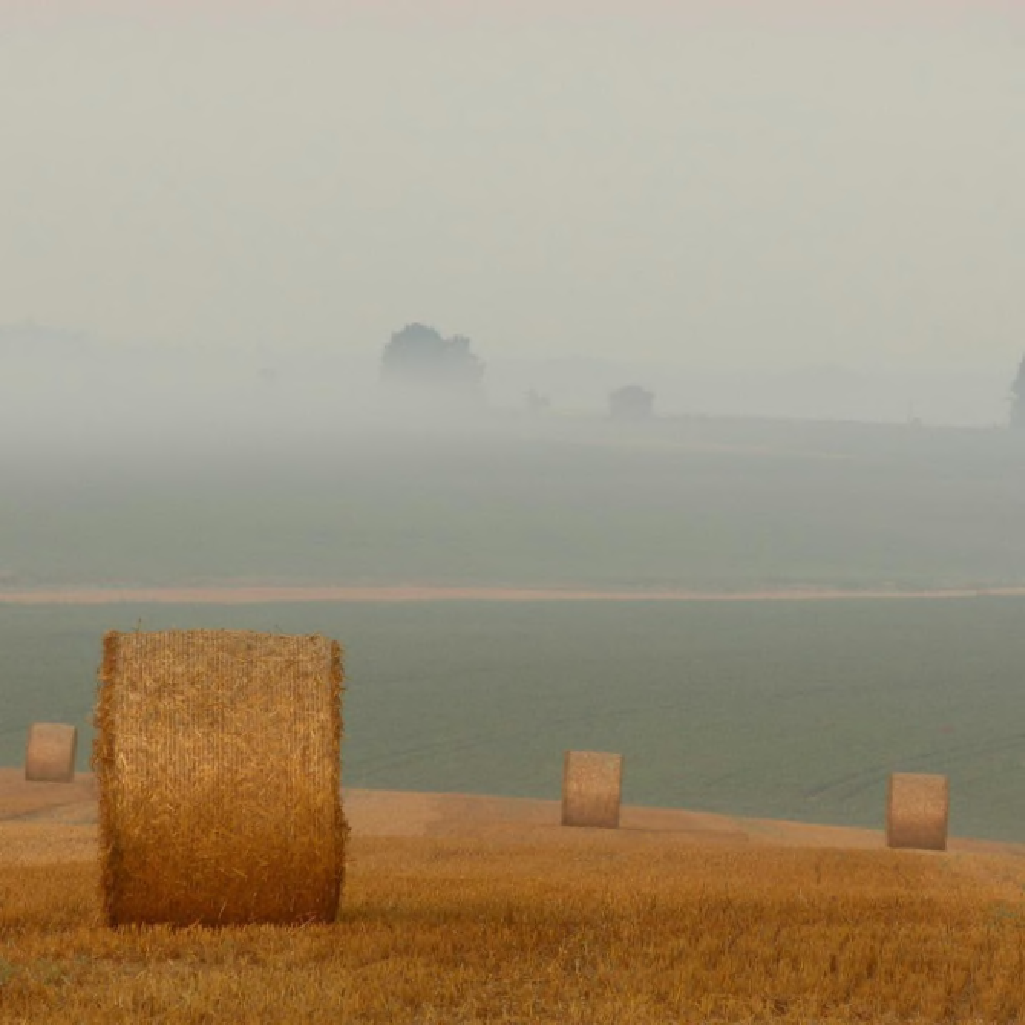
\includegraphics[width=0.4\textwidth]{./RawPictures/stogi.png} }}%
    \caption{Obrazy wejściowe po ujednoliceniu geometrycznym}%
    \label{fig:geo_after_grey1}%
\end{figure}
\FloatBarrier
\begin{figure}[h]
    \centering
    \subfloat[Obraz 1: 1025x1025]{{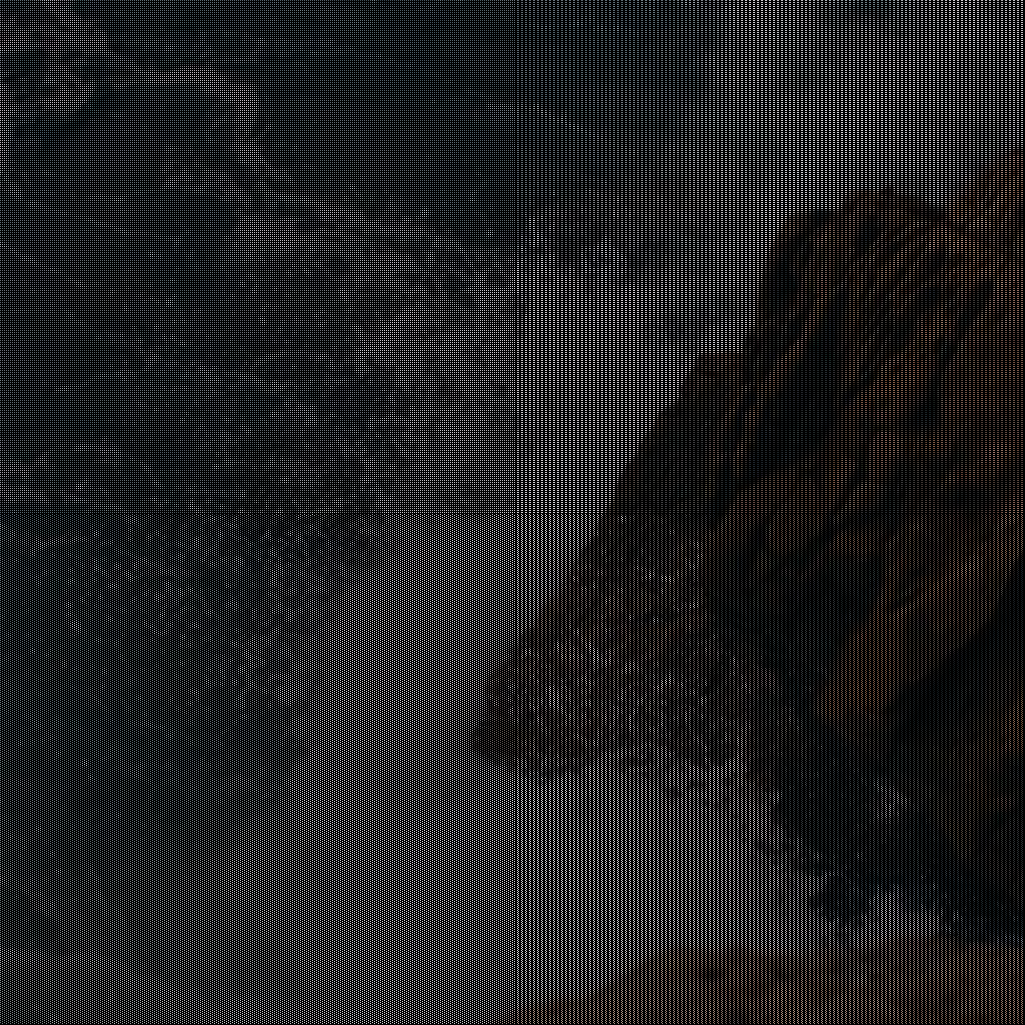
\includegraphics[width=0.4\textwidth]{./ExEffects/1/14/morze_stogi_withoutInterpolation.png} }}%
    \qquad
    \subfloat[Obraz 2: 1025x1025]{{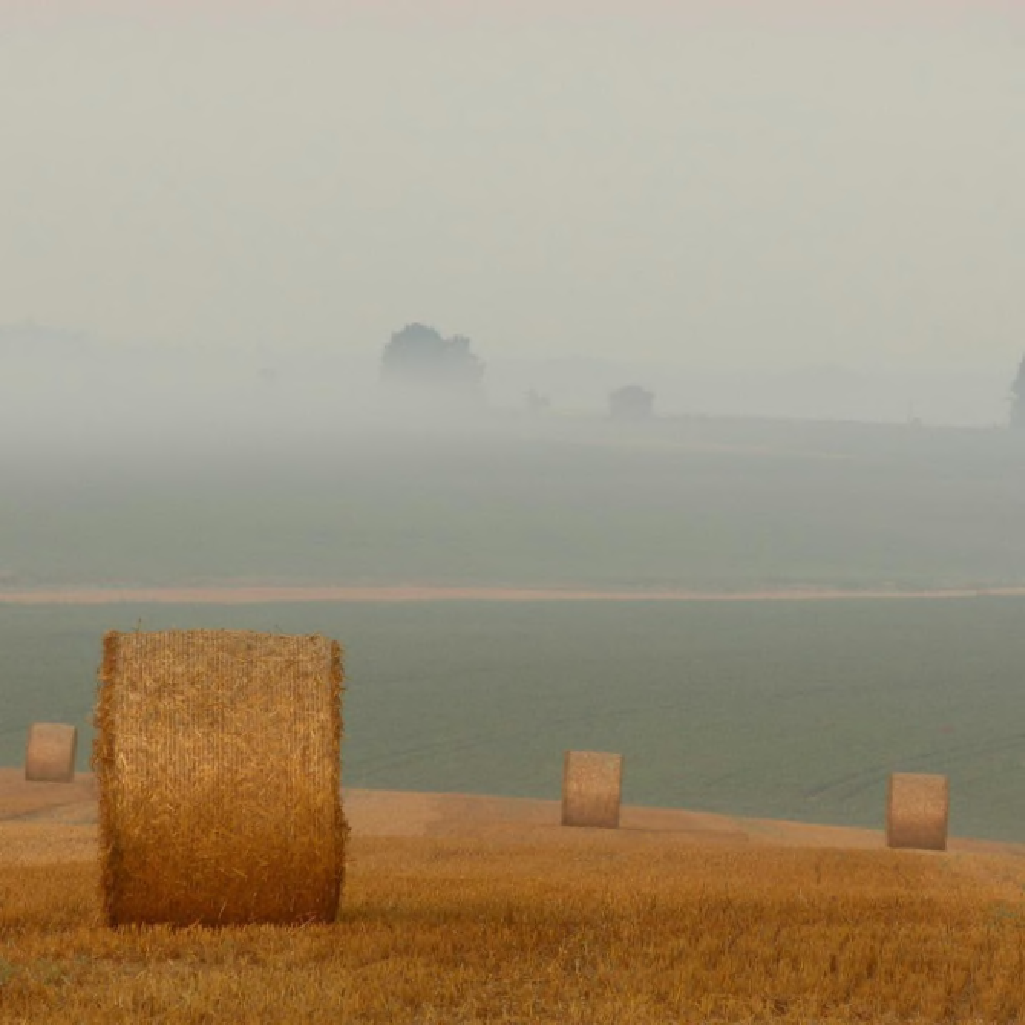
\includegraphics[width=0.4\textwidth]{./RawPictures/stogi.png} }}%
    \caption{Obrazy wyjściowe bez interpolacji}%
    \label{fig:example}%
\end{figure}
\FloatBarrier
\begin{figure}[h]
    \centering
    \subfloat[Obraz 1: 1025x1025]{{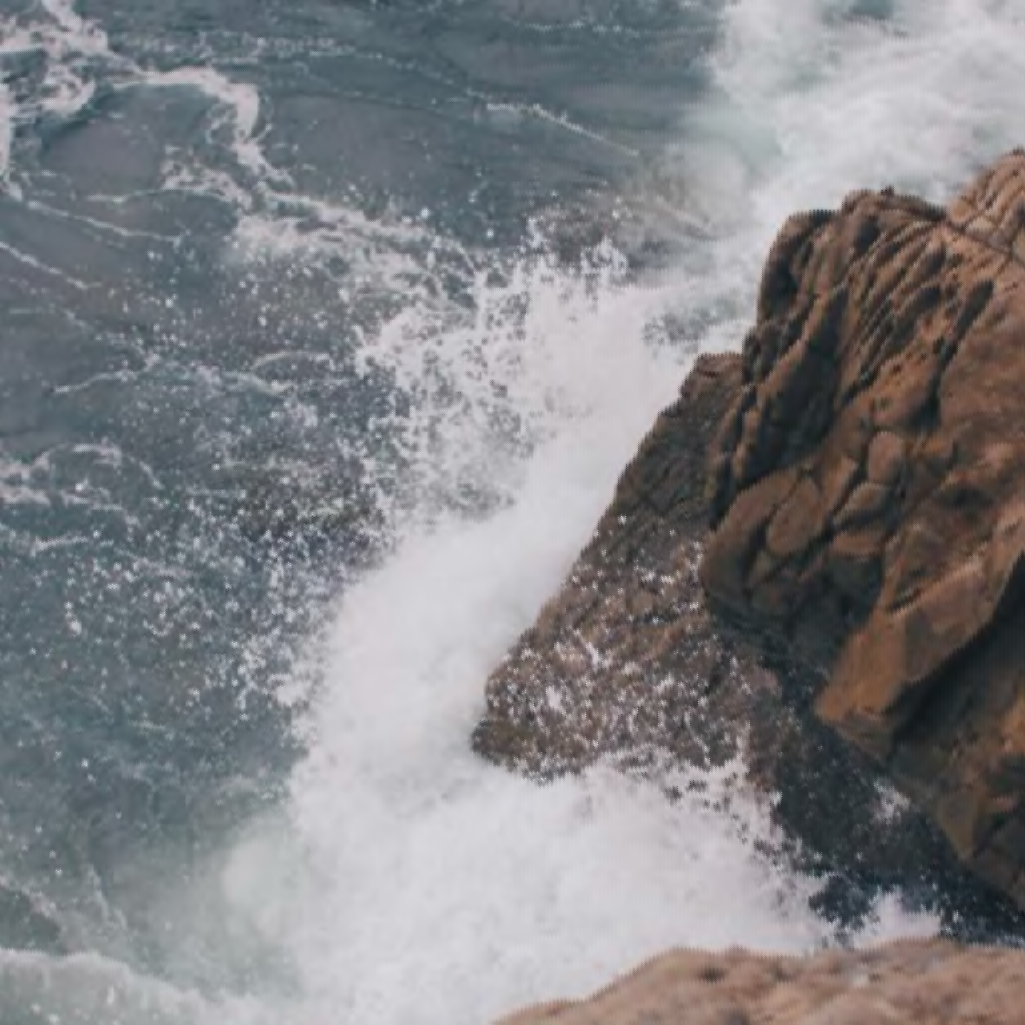
\includegraphics[width=0.4\textwidth]{./ExEffects/1/14/morze_stogi_withInterpolation.png} }}%
    \qquad
    \subfloat[Obraz 2: 1025x1025]{{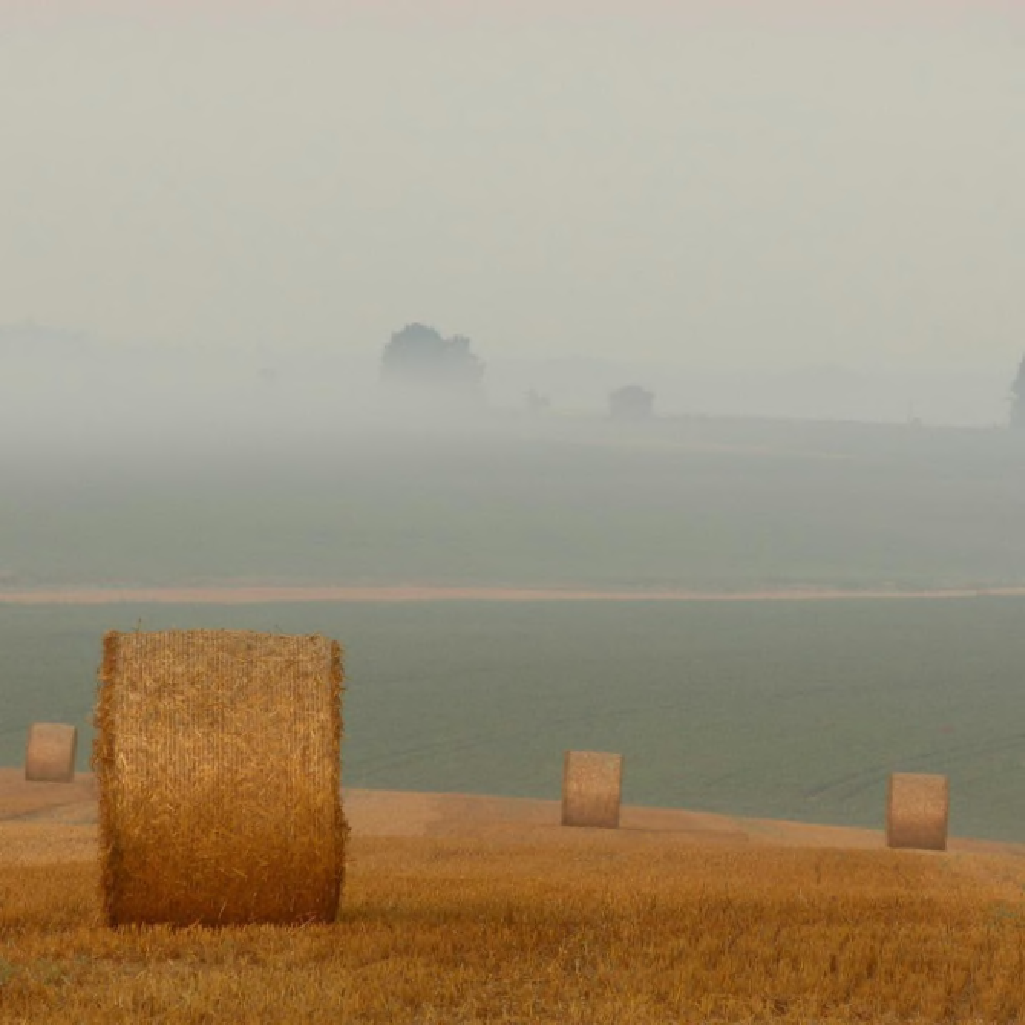
\includegraphics[width=0.4\textwidth]{./RawPictures/stogi.png} }}%
    \caption{Obrazy wyjściowe po interpolacji}%
    \label{fig:example}%
\end{figure}
\FloatBarrier
\subsection*{Kod źródłowy algorytmu}
\begin{lstlisting}[language=Python]
def resolutionUnificationGrey(self):
    print('Beginning of resolution unification for two grey pictures.')
    if self.biggerPicture == 0 and self.smallerPicture == 0:
        print('Both pictures have the same size')
        return 0
    scaleFactorLength = float(self.maxLength / self.minLength)
    scaleFactorWidth = float(self.maxWidth / self.minWidth)
    result = np.zeros((self.maxLength, self.maxWidth), np.uint8)
    for l in range(self.minLength):
        for w in range(self.minWidth):
            if w % 2 == 0:
                pomL = int(scaleFactorLength * l)
                pomW = int(round(scaleFactorWidth * w))
                result[pomL, pomW] = self.matrix[l, w]
            elif w % 2 == 1:
                pomL = int(round(scaleFactorLength * l))
                pomW = int(scaleFactorWidth * w)
                result[pomL, pomW] = self.matrix[l, w]
    # zapisz obraz bez interpolacji
    path = self.ex + self.smallerPictureName + '_' + self.biggerPictureName + '_withoutInterpolation.png'
    self.saver.savePictureFromArray(result, 'L', path)
    # interpolacja
    for l in range(self.maxLength):
        for w in range(self.maxWidth):
            value = 0
            count = 0
            if result[l, w] == 0:
                for lOff in range(-1, 2):
                    for wOff in range(-1, 2):
                        lSave = l if ((l + lOff) > (self.maxLength - 2)) | ((l + lOff) < 0) else (l + lOff)
                        wSave = w if ((w + wOff) > (self.maxWidth - 2)) | ((w + wOff) < 0) else (w + wOff)
                        if result[lSave, wSave] != 0:
                            value += result[lSave, wSave]
                            count += 1
                result[l, w] = value / count
    # zapisz obraz po interpolacji
    path = self.ex + self.smallerPictureName + '_' + self.biggerPictureName + '_withInterpolation.png'
    self.saver.savePictureFromArray(result, 'L', path)
    print('Finished resolution unification.')
\end{lstlisting}

\chapter{Operacje sumowania arytmetycznego obrazów szarych}
Operacje arytmtyczne między pikslami dwóch obrazów sa wykorzystywane w wielu działach przetwarzania obrazów. Przeprowadza się je wykonując operacje na pojedynczych pikslach. Po operacjach arytmetycznych zwykle konieczne jest normalizowanie obrazu wynikowego. W zadaniach do normalizacji wykorzystano wzór:
\[f_{norm}=Z_{rep}[(f-f_{min})/(f_{max}-f_{min})]\]

\section{Sumowanie obrazów szarych z określoną stałą}
\subsection*{Opis algorytmu}
\par Algorytm sumowowania obrazu szarego z określoną stałą polega na daodaniu do każdej wartości pojedynczego piksla określonej stałej. Po operacji sumowania następuje normalizacja obrazu.
\begin{enumerate}
\item Policz sumy wartości każdego piksla ze stałą. Jeżeli suma przekracza 255 to konieczne jest
\begin{itemize}
\item Wybranie największej sumę piksla ze stałą - \(Q_{max}\) 
\item Obliczenie \(D_{max}\) ze wzoru: \(D_{max}[l,w]=(Q_{max}[l,w]-255)\)
\item Obliczenie \(X=D_{max}/255\)
\end{itemize}
\item Policz sumę ze wzoru: \(Q[l,w]=P[l,w]-(P[l, w]*X)+const-(const*X)\)
\end{enumerate}
\subsection*{Efekty wykorzystania algorytmu}
\begin{figure}[h]
    \centering
    \subfloat{{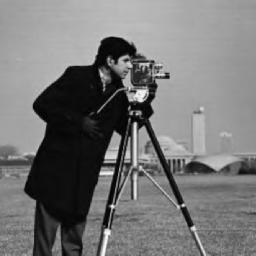
\includegraphics[width=0.3\textwidth]{./RawPictures/fotograf.png} }}%
    \subfloat{{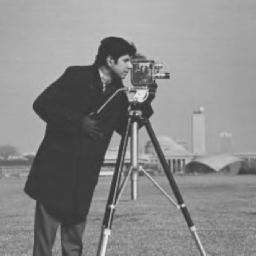
\includegraphics[width=0.3\textwidth]{./ExEffects/2/21/fotograf_constant_70.png} }}%
    \subfloat{{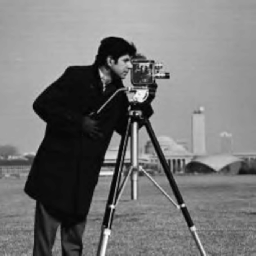
\includegraphics[width=0.3\textwidth]{./ExEffects/2/21/fotograf_constant_70_normalized.png} }}%
    \caption{[Od lewej] Szary obraz wejściowy, obraz po sumowaniu ze stałą 70, obraz po normalizacji}%
    \label{fig:geo_after_grey1}%
\end{figure}
\FloatBarrier
\begin{figure}[h]
    \centering
    \subfloat{{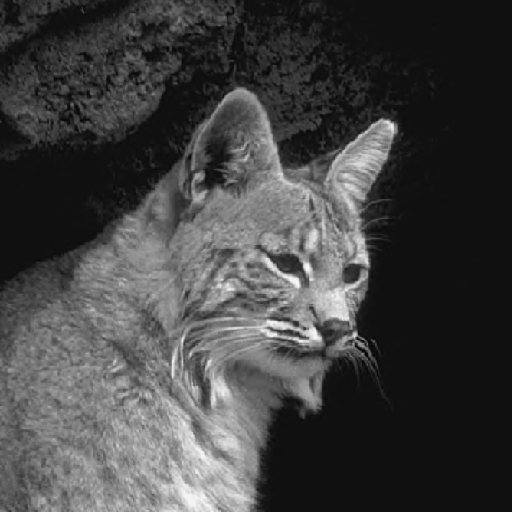
\includegraphics[width=0.3\textwidth]{./RawPictures/rys.png} }}%
    \subfloat{{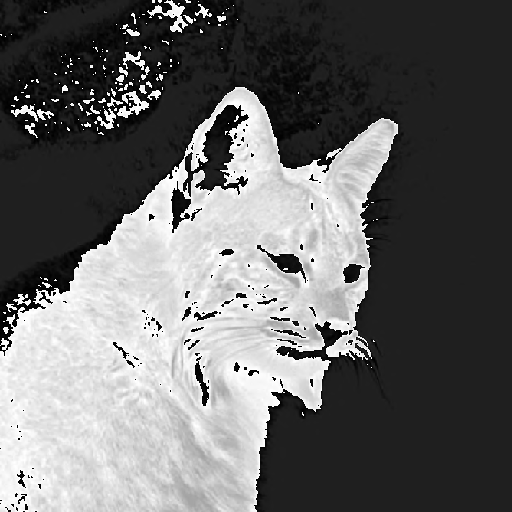
\includegraphics[width=0.3\textwidth]{./ExEffects/2/21/rys_constant_400.png} }}%
    \subfloat{{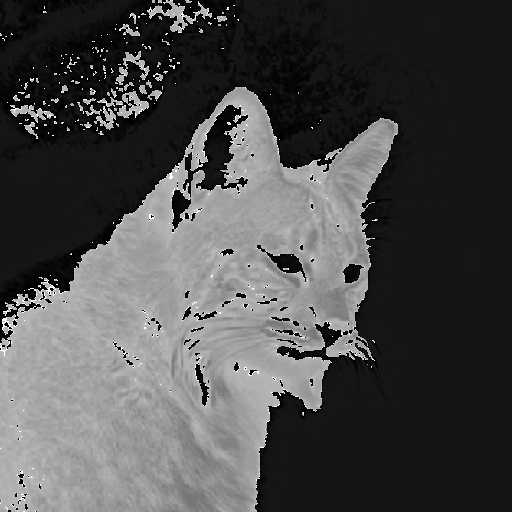
\includegraphics[width=0.3\textwidth]{./ExEffects/2/21/rys_constant_400_normalized.png} }}%
    \caption{[Od lewej] Szary obraz wejściowy, obraz po sumowaniu ze stałą 400, obraz po normalizacji}%
    \label{fig:geo_after_grey1}%
\end{figure}
\FloatBarrier
\subsection*{Kod źródłowy algorytmu}
\begin{lstlisting}[language=Python]
def addConstGrey(self, constant):
    maxBitsColor = self.checkPictureBits(self.pic1)
    length, width, pictureName = self.pic1.getPictureParameters()
    matrix = self.pic1.getGreyMatrix()
    result = np.ones((length, width), np.uint8)
    sumMax = 0
    x = 0
    fmin = maxBitsColor
    fmax = 0
    for l in range(length):
        for w in range(width):
            added = matrix[l, w] + constant
            if sumMax < added:
                sumMax = added
    if sumMax > maxBitsColor:
        x = (sumMax - maxBitsColor) / maxBitsColor
    for l in range(length):
        for w in range(width):
            # Rounded up and assignment of value to the result matrix
            pom = (matrix[l, w] - (matrix[l, w] * x)) + (constant - (constant * x))
            result[l, w] = np.ceil(pom)
            # Search for maximum and minimum
            if fmin > pom:
                fmin = pom
            if fmax < pom:
                fmax = pom
    # save picture with added constant to png file (without normalization)
    path = self.ex + str(pictureName) + '_constant_' + str(constant) + '.png'
    self.saver.savePictureFromArray(result, self.pictureType, path)
    for l in range(length):
        for w in range(width):
            result[l, w] = maxBitsColor*((result[l, w] - fmin) / (fmax - fmin))
    # save picture with added constant to png file (with normalization)
    path = self.ex + str(pictureName) + '_constant_' + str(constant) + '_normalized.png'
    self.saver.savePictureFromArray(result, self.pictureType, path)
\end{lstlisting}

\section{Sumowanie dwóch obrazów szarych}
\subsection*{Opis algorytmu}
\par Algorytm sumowowania obrazu szarego z drugim obrazem szarym jest określone tylko o tych samych wymiarach \(MxN\) i strukturze ich macierzy. Algorytm sumowania obrazu z obrazem polega na dodaniu do wartości piksla z  pierwszego obrazu, wartości odpowiadającego piksla z drugiego obrazu. Po operacji sumowania następuje normalizacja obrazu. Operacja dodawania obrazów są użyteczne przy uśrednianiu obrazów, w celu zredukowania na nich szumu.
\begin{enumerate}
\item Policz sumy wartości każdego piksla obrazu pierwszego \(P1[l,w]\) z odpowiadającym pikslem drugiego obrazu \(P2[l,w]\). Jeżeli suma przekracza 255 to konieczne jest
\begin{itemize}
\item Wybranie największej sumy \(Q_{max}\) 
\item Obliczenie \(D_{max}\) ze wzoru: \(D_{max}[l,w]=(Q_{max}[l,w]-255)\)
\item Obliczenie \(X=D_{max}/255\)
\end{itemize}
\item Policz sumę ze wzoru: \[Q[l,w]=P1[l,w]-(P1[l,w]*X)+P2[l,w]-(P2[l,w]*X)\]
\end{enumerate}
\subsection*{Efekty wykorzystania algorytmu}
\begin{figure}[h]
    \centering
    \subfloat{{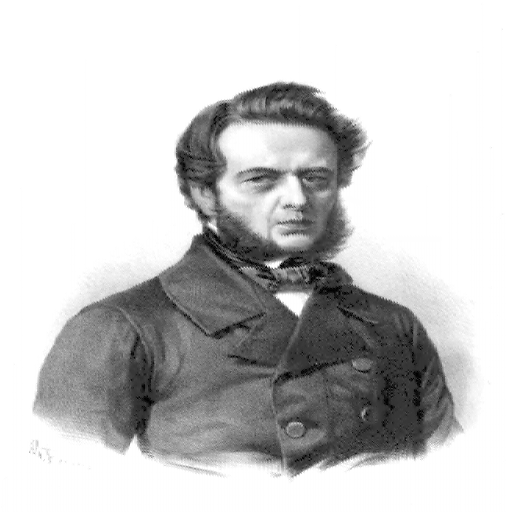
\includegraphics[width=0.4\textwidth]{./ExEffects/1/12/AndrzejZamoyski_rys_withInterpolation.png} }}%
    \subfloat{{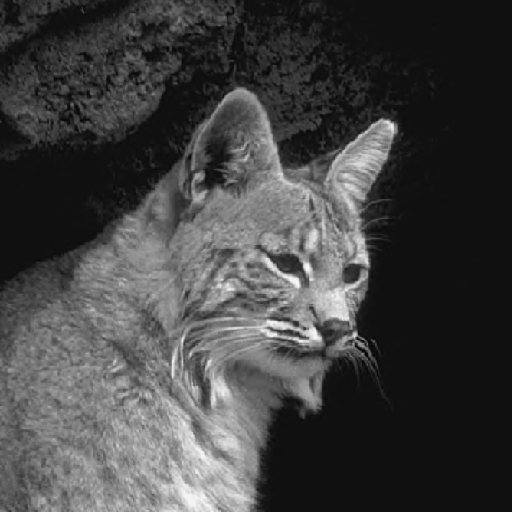
\includegraphics[width=0.4\textwidth]{./RawPictures/rys.png} }}%
    \qquad
    \subfloat{{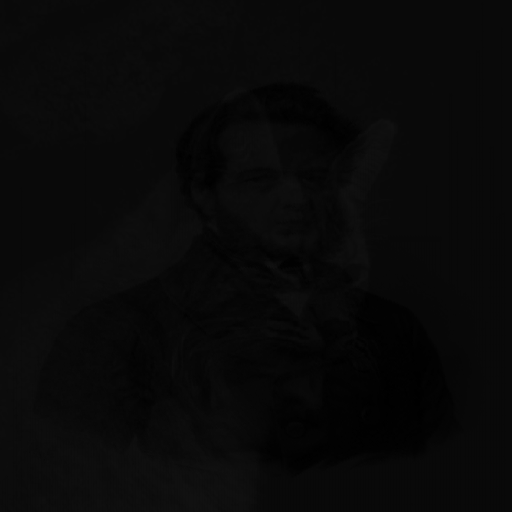
\includegraphics[width=0.4\textwidth]{./ExEffects/2/21/AndrzejZamoyski_added_rys.png} }}%
    \subfloat{{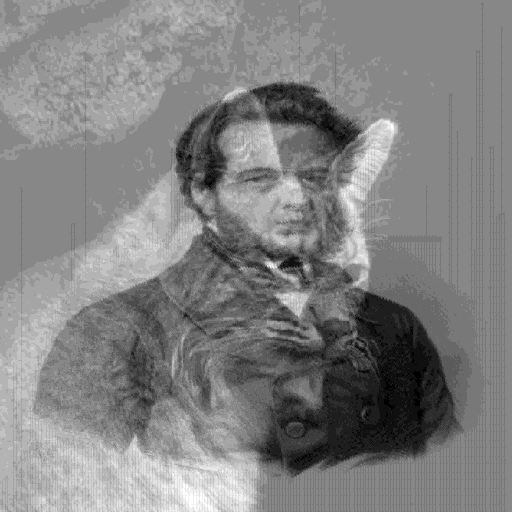
\includegraphics[width=0.4\textwidth]{./ExEffects/2/21/AndrzejZamoyski_added_rys_normalized.png} }}%
    \caption{[Od lewej, rząd 1] Szary obraz wejściowy 1, szary obraz wejściowy 2 [Od lewej, rząd 2] Obraz po sumowaniu obrazów 1 i 2, obraz po normalizacji}%
    \label{fig:geo_after_grey1}%
\end{figure}
\FloatBarrier
\begin{figure}[h]
    \centering
    \subfloat{{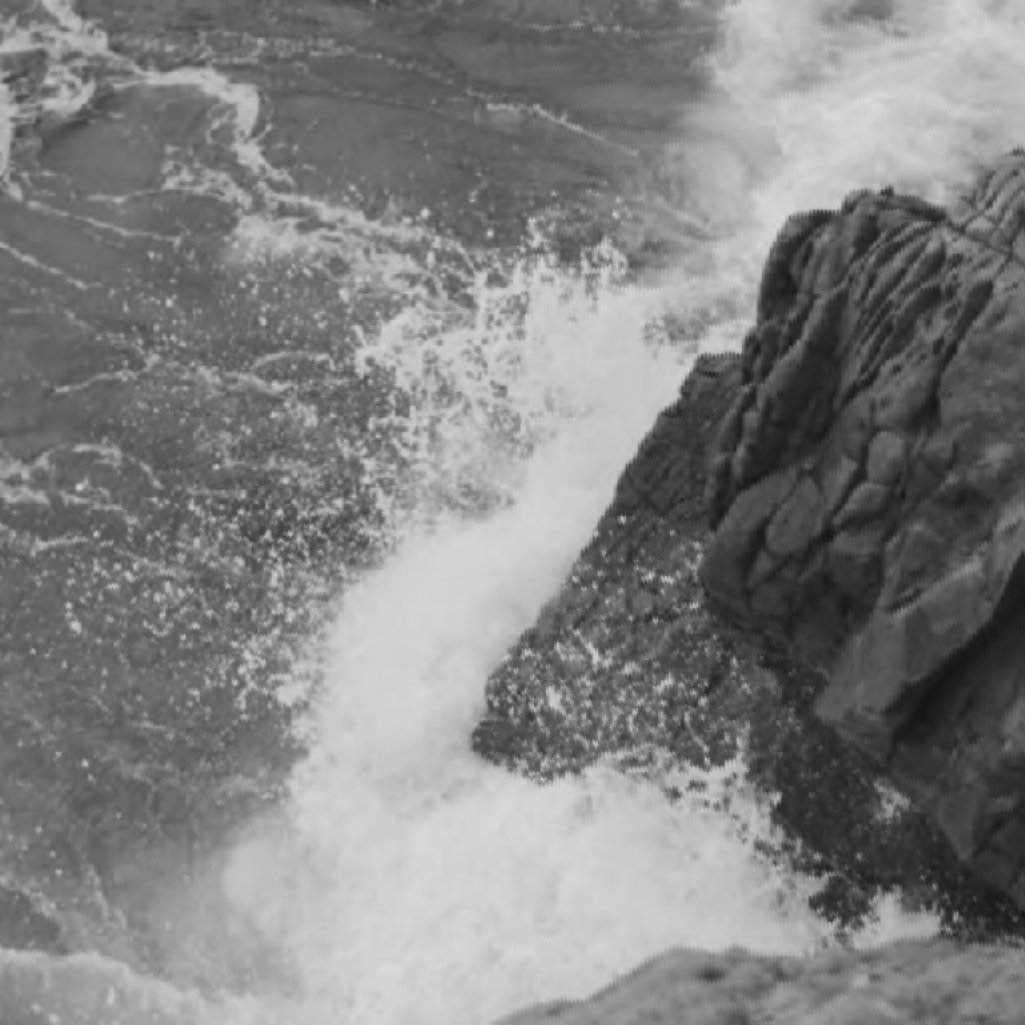
\includegraphics[width=0.4\textwidth]{./ExEffects/1/12/morze-szare_stogi-szare_withInterpolation.png} }}%
    \subfloat{{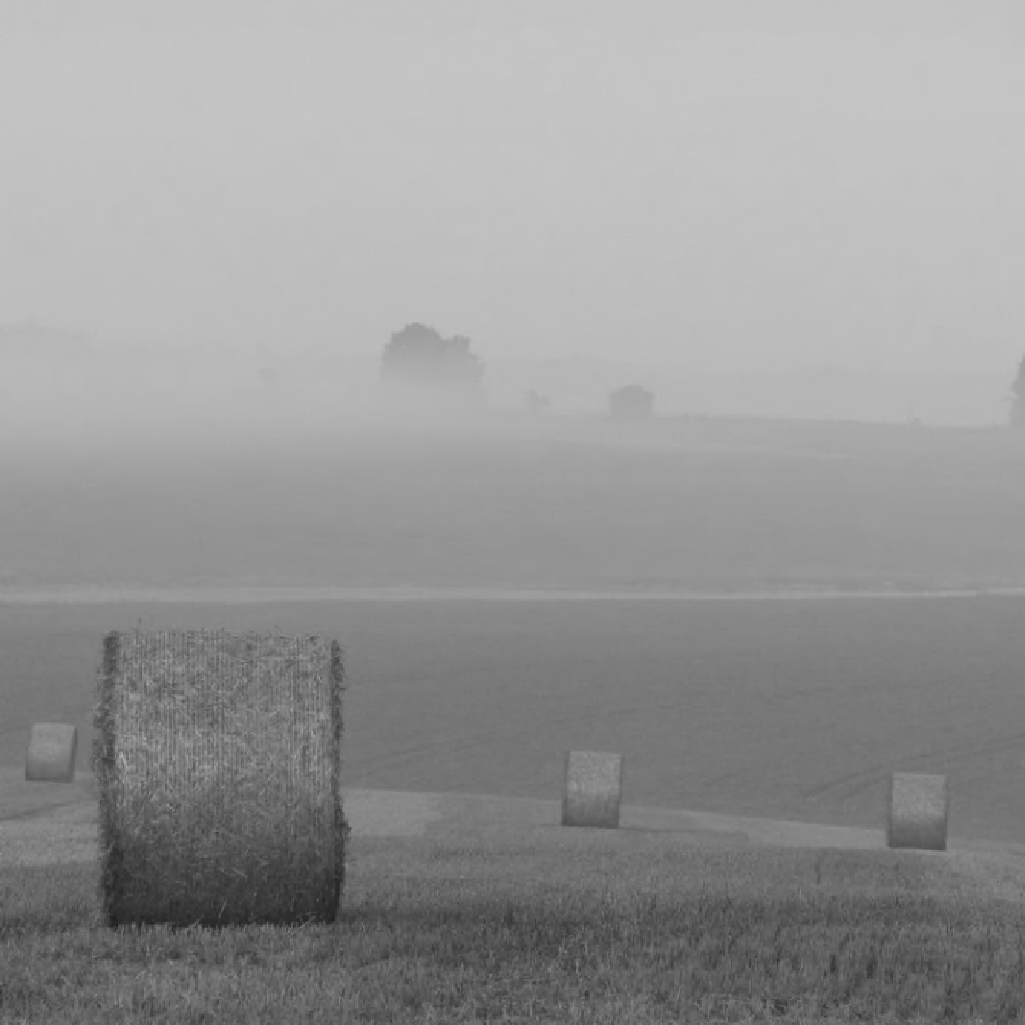
\includegraphics[width=0.4\textwidth]{./RawPictures/stogi-szare.png} }}%
    \qquad
    \subfloat{{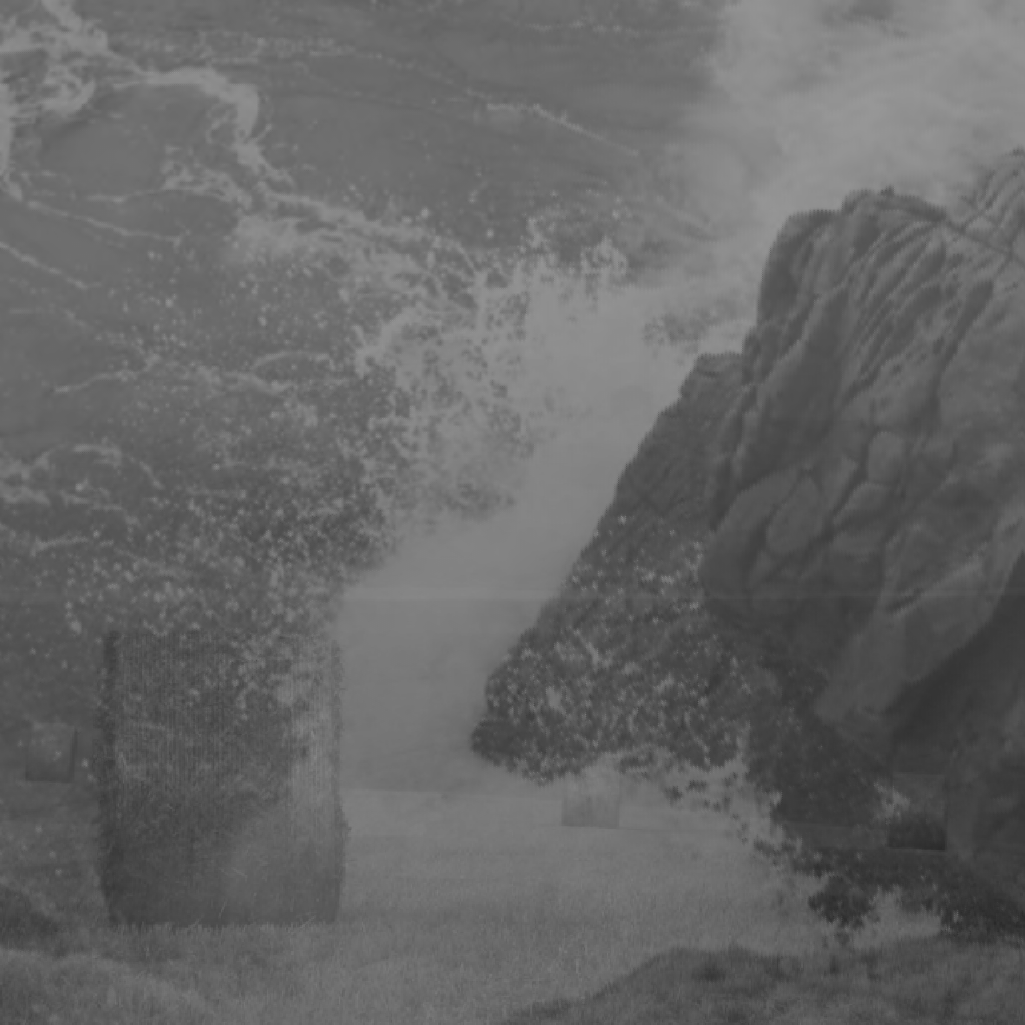
\includegraphics[width=0.4\textwidth]{./ExEffects/2/21/morze-szare_added_stogi-szare.png} }}%
    \subfloat{{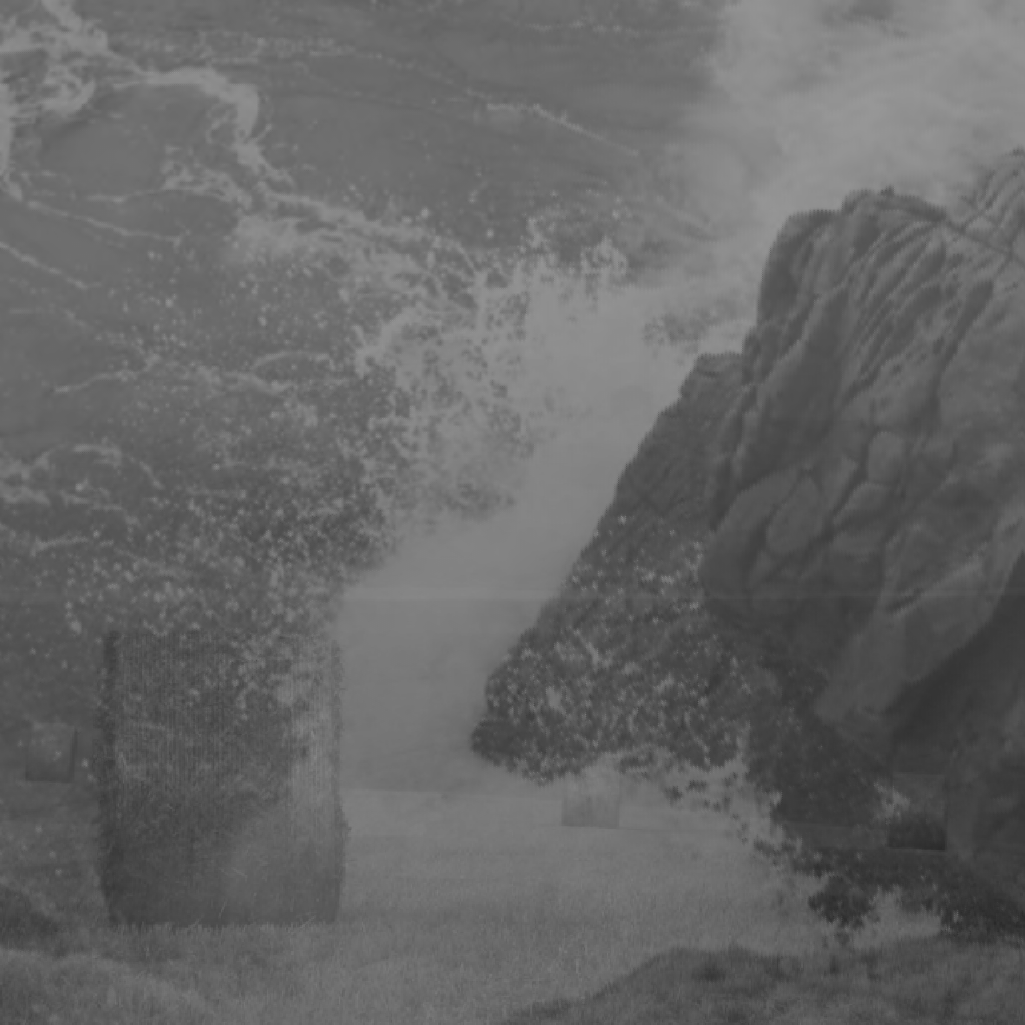
\includegraphics[width=0.4\textwidth]{./ExEffects/2/21/morze-szare_added_stogi-szare_normalized.png} }}%
    \caption{[Od lewej, rząd 1] Szary obraz wejściowy 1, szary obraz wejściowy 2 [Od lewej, rząd 2] Obraz po sumowaniu obrazów 1 i 2, obraz po normalizacji}%
    \label{fig:geo_after_grey1}%
\end{figure}
\FloatBarrier
\subsection*{Kod źródłowy algorytmu}
\begin{lstlisting}[language=Python]
def addPictureGrey(self):
    if self.checkPictureBits(self.pic1) == self.checkPictureBits(self.pic2):
        maxBitsColor = self.checkPictureBits(self.pic2)
    # check if pictures have same sizes, if not unify them
    compare = Comparer()
    biggerPicture, smallerPicture = compare.comparePictures(self.pic1, self.pic2)
    if biggerPicture != 0 and smallerPicture != 0:
        self.pic1, self.pic2 = self.getUnifiedPictures()
    # get the values
    tempName = smallerPicture.getPictureName()
    length1, width1, pictureName1 = self.pic1.getPictureParameters()
    matrix1 = self.pic1.getGreyMatrix()
    length2, width2, pictureName2 = self.pic2.getPictureParameters()
    matrix2 = self.pic2.getGreyMatrix()
    pictureName1 = tempName

    sumMax = 0
    x = 0
    fmax = 0
    fmin = maxBitsColor

    result = np.zeros((length1, width1), np.uint8)

    for l in range(length1):
        for w in range(width1):
            added = int(matrix1[l, w]) + int(matrix2[l, w])
            if sumMax < added:
                sumMax = added

    if sumMax > maxBitsColor:
        x = (sumMax - maxBitsColor) / maxBitsColor

    for l in range(length1):
        for w in range(width1):
            # Rounded up and assignment of value to the result matrix
            pom = int(matrix1[l, w] - (matrix1[l, w] * x)) + int(matrix2[l, w] - (matrix2[l, w] * x))
            result[l, w] = np.ceil(int(pom))
            # Search for maximum and minimum
            if fmin > pom:
                fmin = pom
            if fmax < pom:
                fmax = pom

    # save picture with added constant to png file (without normalization)
    path = self.ex + str(pictureName1) + '_added_' + str(pictureName2) + '.png'
    self.saver.savePictureFromArray(result, self.pictureType, path)

    normalized = np.zeros((length1, width1), np.uint8)
    for l in range(length1):
        for w in range(width1):
            normalized[l, w] = maxBitsColor*((result[l, w] - fmin) / (fmax - fmin))

    # save picture with added constant to png file (with normalization)
    path = self.ex + str(pictureName1) + '_added_' + str(pictureName2) + '_normalized.png'
    self.saver.savePictureFromArray(result, self.pictureType, path)
\end{lstlisting}

\section{Mnożenie obrazów szarych przez określoną stałą}
\subsection*{Opis algorytmu}
\par Algorytm mnożenia obrazu szarego przez określoną stałą polega na przemnożeniu każdego elementu obrazu (piksla) przez określoną stałą (skalar). Dla wszystkich piksli w obrazie wykonaj:
\begin{enumerate}
\item Jeżeli wartość piksla jest równa 255 to składowa wynikowa otrzymuje wartość stałej.
\item Jeżeli wartość piksla jest równa 0 to składowa wynikowa otrzymuje wartość 0.
\item Jeżeli wartość piksla jest inna niż 255 lub 0 to składowa wynikowa otrzymuje wartość poprzez pomnożenie wartości piksla przez skalar, podzielenie przez 255 i zaokrąglenie do liczby całkowitej.
\end{enumerate}
\subsection*{Efekty wykorzystania algorytmu}
\begin{figure}[h]
    \centering
    \subfloat{{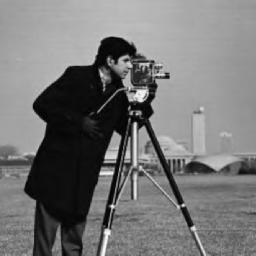
\includegraphics[width=0.3\textwidth]{./RawPictures/fotograf.png} }}%
    \subfloat{{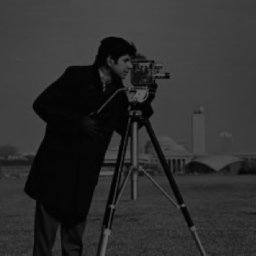
\includegraphics[width=0.3\textwidth]{./ExEffects/2/22/fotograf_constant_100.png} }}%
    \subfloat{{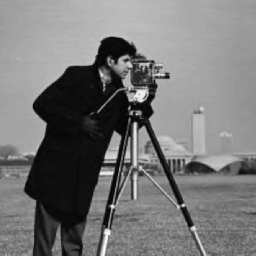
\includegraphics[width=0.3\textwidth]{./ExEffects/2/22/fotograf_constant_100_normalized.png} }}%
    \caption{[Od lewej] Szary obraz wejściowy, obraz po sumowaniu ze stałą 100, obraz po normalizacji}%
    \label{fig:geo_after_grey1}%
\end{figure}
\FloatBarrier
\begin{figure}[h]
    \centering
    \subfloat{{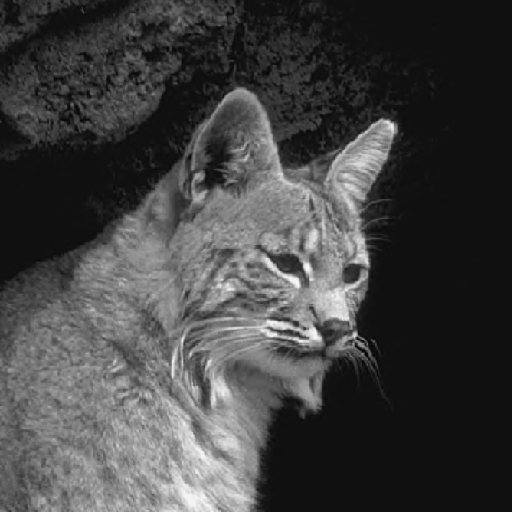
\includegraphics[width=0.3\textwidth]{./RawPictures/rys.png} }}%
    \subfloat{{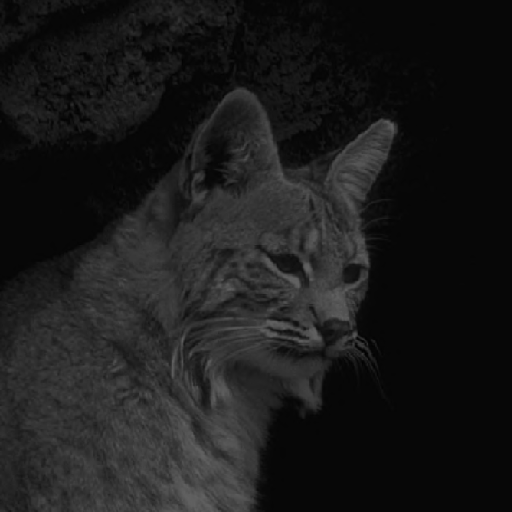
\includegraphics[width=0.3\textwidth]{./ExEffects/2/22/rys_constant_100.png} }}%
    \subfloat{{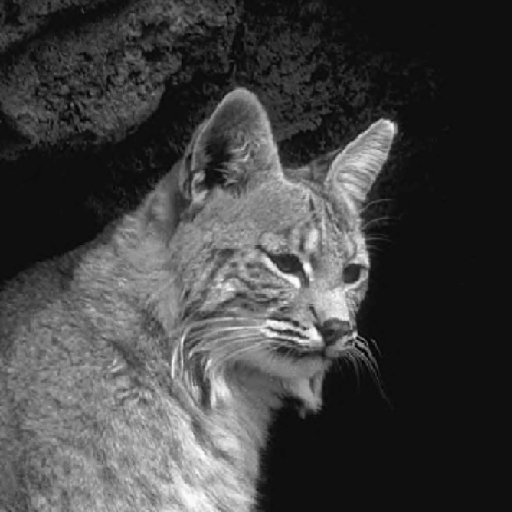
\includegraphics[width=0.3\textwidth]{./ExEffects/2/22/rys_constant_100_normalized.png} }}%
    \caption{[Od lewej] Szary obraz wejściowy, obraz po sumowaniu ze stałą 100, obraz po normalizacji}%
    \label{fig:geo_after_grey1}%
\end{figure}
\FloatBarrier
\subsection*{Kod źródłowy algorytmu}
\begin{lstlisting}[language=Python]
def multiplyConstGrey(self, constant):
    maxBitsColor = self.checkPictureBits(self.pic1)
    length, width, matrix, pictureName = self.getPictureParameters(self.pic1)
    result = np.ones((length, width), np.uint8)
    fmin = maxBitsColor
    fmax = 0
    for l in range(length):
        for w in range(width):
            pom = matrix[l, w]
            if pom == maxBitsColor:
                result[l, w] = maxBitsColor
            elif pom == 0:
                result[l, w] = 0
            else:
                result[l, w] = np.ceil(((matrix[l, w] * constant) / maxBitsColor))
            # Search for maximum and minimum
            if fmin > result[l, w]:
                fmin = result[l, w]
            if fmax < result[l, w]:
                fmax = result[l, w]
    # save picture with added constant to png file (without normalization)
    path = self.ex + str(pictureName) + '_constant_' + str(constant) + '.png'
    self.saver.savePictureFromArray(result, self.pictureType, path)
    for l in range(length):
        for w in range(width):
            result[l, w] = maxBitsColor*((result[l, w] - fmin) / (fmax - fmin))
    # save picture with added constant to png file (with normalization)
    path = self.ex + str(pictureName) + '_constant_' + str(constant) + '_normalized.png'
    self.saver.savePictureFromArray(result, self.pictureType, path)
\end{lstlisting}

\section{Mnożenie obrazu przez inny obraz}
\subsection*{Opis algorytmu}
\par Algorytm mnożenia obrazu szarego przez drugi szary obraz o tych samych wymiarach \(MxN\) i strukturze ich macierzy polega na przemnożeniu wartości piksla z pierwszego obrazu przez wartość odpowiadającego piksla z drugiego obrazu. Po operacji mnożenia następuje normalizacja obrazu. Dla każdego piksla pierwszego obrazu wykonaj następujące czynności:
\begin{enumerate}
\item Jeżeli wartość piksla \(P1[l,w]\) jest równa 255 to składowa wynikowa otrzymuje wartość odpowiadającego piksla drugiego obrazu \(P2[l,w]\).
\item Jeżeli wartość piksla \(P1[l,w]\) jest równa 0 to składowa wynikowa otrzymuje wartość 0.
\item Jeżeli wartość piksla \(P1[l,w]\) jest inna niż 255 lub 0 to składowa wynikowa otrzymuje wartość poprzez pomnożenie wartości piksla \(P1[l,w]\) przez odpowiadający piksel \(P2[l,w]\), podzielenie przez 255 i zaokrąglenie do liczby całkowitej.
\end{enumerate}
\subsection*{Efekty wykorzystania algorytmu}
\begin{figure}[h]
    \centering
    \subfloat{{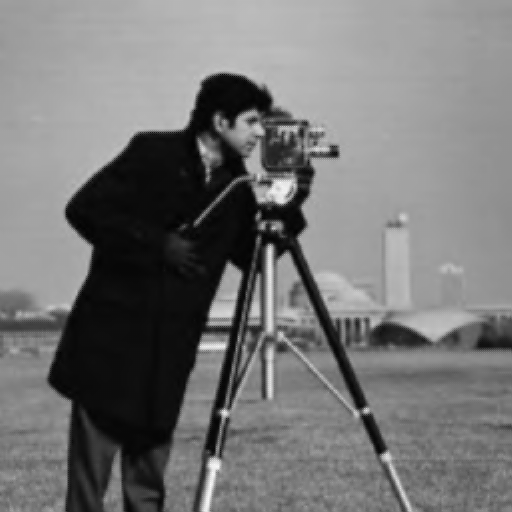
\includegraphics[width=0.4\textwidth]{./ExEffects/1/12/fotograf_rys_withInterpolation.png} }}%
    \subfloat{{\includegraphics[width=0.4\textwidth]{./RawPictures/rys.png} }}%
    \qquad
    \subfloat{{\includegraphics[width=0.4\textwidth]{./ExEffects/2/22/fotograf_multiplied_rys.png} }}%
    \subfloat{{\includegraphics[width=0.4\textwidth]{./ExEffects/2/22/fotograf_multiplied_rys_normalized.png} }}%
    \caption{[Od lewej, rząd 1] Szary obraz wejściowy 1, szary obraz wejściowy 2 [Od lewej, rząd 2] Obraz po sumowaniu obrazów 1 i 2, obraz po normalizacji}%
    \label{fig:geo_after_grey1}%
\end{figure}
\FloatBarrier
\begin{figure}[h]
    \centering
    \subfloat{{\includegraphics[width=0.4\textwidth]{./ExEffects/1/12/fotograf_AndrzejZamoyski_withInterpolation.png} }}%
    \subfloat{{\includegraphics[width=0.4\textwidth]{./RawPictures/AndrzejZamoyski.png} }}%
    \qquad
    \subfloat{{\includegraphics[width=0.4\textwidth]{./ExEffects/2/22/fotograf_multiplied_AndrzejZamoyski.png} }}%
    \subfloat{{\includegraphics[width=0.4\textwidth]{./ExEffects/2/22/fotograf_multiplied_AndrzejZamoyski_normalized.png} }}%
    \caption{[Od lewej, rząd 1] Szary obraz wejściowy 1, szary obraz wejściowy 2 [Od lewej, rząd 2] Obraz po sumowaniu obrazów 1 i 2, obraz po normalizacji}%
    \label{fig:geo_after_grey1}%
\end{figure}
\FloatBarrier
\subsection*{Kod źródłowy algorytmu}
\begin{lstlisting}[language=Python]
def multiplyPicturesGrey(self):
    if self.checkPictureBits(self.pic1) == self.checkPictureBits(self.pic2):
        maxBitsColor = self.checkPictureBits(self.pic2)
    # check if pictures have same sizes, if not unify them
    compare = Comparer()
    biggerPicture, smallerPicture = compare.comparePictures(self.pic1, self.pic2)
    if biggerPicture != 0 and smallerPicture != 0:
        self.pic1, self.pic2 = self.getUnifiedPictures()
    # get the values
    tempName = smallerPicture.getPictureName()
    length1, width1, matrix1, pictureName1 = self.getPictureParameters(self.pic1)
    length2, width2, matrix2, pictureName2 = self.getPictureParameters(self.pic2)
    pictureName1 = tempName

    result = np.ones((length1, width1), np.uint8)

    fmin = maxBitsColor
    fmax = 0

    for l in range(length1):
        for w in range(width1):
            if matrix1[l, w] == maxBitsColor:
                result[l, w] = matrix2[l, w]
            elif matrix1[l, w] == 0:
                result[l, w] = 0
            else:
                result[l, w] = np.ceil(((int(matrix1[l, w]) * int(matrix2[l, w])) / maxBitsColor))
            # Search for maximum and minimum
            if fmin > result[l, w]:
                fmin = result[l, w]

            if fmax < result[l, w]:
                fmax = result[l, w]

    # save picture multiplied by picture to png file (without normalization)
    path = self.ex + str(pictureName1) + '_multiplied_' + str(pictureName2) + '.png'
    self.saver.savePictureFromArray(result, self.pictureType, path)

    for l in range(length1):
        for w in range(width1):
            result[l, w] = maxBitsColor*((result[l, w] - fmin) / (fmax - fmin))

    # save picture multiplied by picture to png file (with normalization)
    path = self.ex + str(pictureName1) + '_multiplied_' + str(pictureName2) + '_normalized.png'
    self.saver.savePictureFromArray(result, self.pictureType, path)
\end{lstlisting}

\section{Mieszanie obrazów z określonym współczynnikiem}
\subsection*{Opis algorytmu}
\par Mieszanie dwóch obrazów polega na sumowaniu ich z wagami \(\alpha\) i \(1-\alpha\) według wzoru: \[f_{m}=f\alpha+f^{I}(1-\alpha)\] gdzie \(\alpha\in[0,1]\). Płynna zmiana parametru \(\alpha\) w przedziale \([0,1]\) powoduje efekt przechodzenia obrazu \(f\) w obraz \(f^{I}\).
\begin{enumerate}
\item Weź dwa obrazy szare o takim samym rozmiarze (po ujednoliceniu rozdzielczościowym) \(P_{1}\) i \(P_{2}\).
\item Określ współczynnik mieszania obrazów \(\alpha\) wyrażony jako liczba rzeczywista z przedziału \([0,1]\), gdzie 0 reprezentuje przezroczystość, a 1 reprezentuje nieprzezroczystość.
\item Dla wszystkich piksli w obrazach wejściowych wykonaj: \[Q[l,w]=\alpha*P_{1}[l,w]+(1-\alpha)*P_{2}[l,w]\]
\end{enumerate}
\subsection*{Efekty wykorzystania algorytmu}
\begin{figure}[h]
    \centering
    \subfloat{{\includegraphics[width=0.4\textwidth]{./ExEffects/1/12/fotograf_rys_withInterpolation.png} }}%
    \subfloat{{\includegraphics[width=0.4\textwidth]{./RawPictures/rys.png} }}%
    \qquad
    \subfloat{{\includegraphics[width=0.4\textwidth]{./ExEffects/2/23/fotograf_blended_0.8_rys.png} }}%
    \subfloat{{\includegraphics[width=0.4\textwidth]{./ExEffects/2/23/fotograf_blended_0.8_rys_normalized.png} }}%
    \caption{[Od lewej, rząd 1] Szary obraz wejściowy 1, szary obraz wejściowy 2 [Od lewej, rząd 2] Obraz po mieszaniu ze współczynnikiem \(\alpha=0.8\), obraz po normalizacji}%
    \label{fig:geo_after_grey1}%
\end{figure}
\FloatBarrier
\begin{figure}[h]
    \centering
    \subfloat{{\includegraphics[width=0.4\textwidth]{./ExEffects/1/12/fotograf_AndrzejZamoyski_withInterpolation.png} }}%
    \subfloat{{\includegraphics[width=0.4\textwidth]{./RawPictures/AndrzejZamoyski.png} }}%
    \qquad
    \subfloat{{\includegraphics[width=0.4\textwidth]{./ExEffects/2/23/fotograf_blended_0.3_AndrzejZamoyski.png} }}%
    \subfloat{{\includegraphics[width=0.4\textwidth]{./ExEffects/2/23/fotograf_blended_0.3_AndrzejZamoyski_normalized.png} }}%
    \caption{[Od lewej, rząd 1] Szary obraz wejściowy 1, szary obraz wejściowy 2 [Od lewej, rząd 2] Obraz po mieszaniu ze współczynnikiem \(\alpha=0.3\), obraz po normalizacji}%
    \label{fig:geo_after_grey1}%
\end{figure}
\FloatBarrier
\subsection*{Kod źródłowy algorytmu}
\begin{lstlisting}[language=Python]
def getUnifiedPictures(self):
        resolutionUni = ResolutionUnificationGrey(self.name1, self.name2)
        resolutionUni.resolutionUnificationGrey()
        pic1Path, pic2Path = resolutionUni.getOutputPaths()
        pic1 = ImageHelper(pic1Path, self.pictureType)
        pic2 = ImageHelper(pic2Path, self.pictureType)
        return pic1, pic2
def blendPictures(self, alfa):
        if self.checkPictureBits(self.pic1) == self.checkPictureBits(self.pic2):
            maxBitsColor = self.checkPictureBits(self.pic2)
        # check if pictures have same sizes, if not unify them
        compare = Comparer()
        biggerPicture, smallerPicture = compare.comparePictures(self.pic1, self.pic2)
        if biggerPicture != 0 and smallerPicture != 0:
            self.pic1, self.pic2 = self.getUnifiedPictures()
        # get the values
        tempName = smallerPicture.getPictureName()
        length1, width1, matrix1, pictureName1 = self.getPictureParameters(self.pic1)
        length2, width2, matrix2, pictureName2 = self.getPictureParameters(self.pic2)
        pictureName1 = tempName

        result = np.ones((length1, width1), np.uint8)

        fmin = maxBitsColor
        fmax = 0

        for l in range(length1):
            for w in range(width1):
                pom = float(matrix1[l, w]) * alfa + float(matrix2[l, w]) * (1 - alfa)
                result[l, w] = np.ceil(pom)

                # Search for maximum and minimum
                if fmin > pom:
                    fmin = pom
                if fmax < pom:
                    fmax = pom

        # save picture multiplied by picture to png file (without normalization)
        path = self.ex + str(pictureName1) + '_blended_' + str(alfa) + '_' + str(pictureName2) + '.png'
        self.saver.savePictureFromArray(result, self.pictureType, path)

        for l in range(length1):
            for w in range(width1):
                result[l, w] = maxBitsColor*((result[l, w] - fmin) / (fmax - fmin))

        # save picture multiplied by picture to png file (with normalization)
        path = self.ex + str(pictureName1) + '_blended_' + str(alfa) + '_' + str(pictureName2) + '_normalized.png'
        self.saver.savePictureFromArray(result, self.pictureType, path)
\end{lstlisting}

\section{Potęgowanie obrazu z zadaną potęgą}
\subsection*{Opis algorytmu}
\par Algorytm potęgowania obrazu szarego do określoną stałej jest szczególnym przypadkiem mnożenia obrazów. Aby uniknąć wykroczenia poza zakres, skorzystano ze znormalizowanego wzoru: \[f_{m}=255*\Big(\frac{f(x,y)}{f_{max}}\Big)^{\alpha},  \alpha>0\]
\subsection*{Efekty wykorzystania algorytmu}
\begin{figure}[h]
    \centering
    \subfloat{{\includegraphics[width=0.3\textwidth]{./RawPictures/fotograf.png} }}%
    \subfloat{{\includegraphics[width=0.3\textwidth]{./ExEffects/2/24/fotograf_power_2.png} }}%
    \subfloat{{\includegraphics[width=0.3\textwidth]{./ExEffects/2/24/fotograf_power_2_normalized.png} }}%
    \caption{[Od lewej] Szary obraz wejściowy, obraz po podniesieniu do potęgi \(\alpha=2\), obraz po normalizacji}%
    \label{fig:geo_after_grey1}%
\end{figure}
\FloatBarrier
\begin{figure}[h]
    \centering
    \subfloat{{\includegraphics[width=0.3\textwidth]{./RawPictures/rys.png} }}%
    \subfloat{{\includegraphics[width=0.3\textwidth]{./ExEffects/2/24/rys_power_3.png} }}%
    \subfloat{{\includegraphics[width=0.3\textwidth]{./ExEffects/2/24/rys_power_3_normalized.png} }}%
    \caption{[Od lewej] Szary obraz wejściowy, obraz po podniesieniu do potęgi \(\alpha=3\), obraz po normalizacji}%
    \label{fig:geo_after_grey1}%
\end{figure}
\FloatBarrier
\subsection*{Kod źródłowy algorytmu}
\begin{lstlisting}[language=Python]
def raiseToPower(self, power):
        length, width, pictureName = self.pic.getPictureParameters()
        matrix = self.pic.getGreyMatrix()
        result = np.zeros((length, width), np.uint8)

        maxPicture = 0
        fmin = maxBitsColor
        fmax = 0

        for l in range(length):
            for w in range(width):
                pom = matrix[l, w]
                if maxPicture < pom:
                    maxPicture = pom

        for l in range(length):
            for w in range(width):
                pom = matrix[l, w]
                if pom == maxBitsColor:
                    pom = maxBitsColor
                elif pom == 0:
                    pom = 0
                else:
                    pom = np.power(int(pom) / maxPicture, power) * maxBitsColor
                result[l, w] = np.ceil(pom)
                # Search for maximum and minimum
                if fmin > pom:
                    fmin = pom

                if fmax < pom:
                    fmax = pom

        # save picture raised to constant power to png file (without normalization)
        path = self.ex + str(pictureName) + '_power_' + str(power) + '.png'
        self.saver.savePictureFromArray(result, self.pictureType, path)

        for l in range(length):
            for w in range(width):
                result[l, w] = maxBitsColor * ((result[l, w] - fmin) / (fmax - fmin))

        # save picture raised to constant power to png file (with normalization)
        path = self.ex + str(pictureName) + '_power_' + str(power) + '_normalized.png'
        self.saver.savePictureFromArray(result, self.pictureType, path)
\end{lstlisting}

\section{Dzielenie obrazów szarych przez zadaną stałą}
\subsection*{Opis algorytmu}
\par Algorytm dzielenia obrazu szarego przez określoną stałą służy korekcji cieniowania między poziomami szarości obrazu. Aby zastosować algorytm dla każdego piksla obrazu wykonaj:
\begin{enumerate}
\item Policz sumę piksla ze stałą.
\item Spośród obliczonych sum wybierz \(Q_{max}\) - największą sumę.
\item Wartość wynikową policz z następującego wzoru: \[Q[l,w]=(S*255)/Q_{max}\]Wynik zaokrąglij w górę do najbliższej liczby całkowitej.
\end{enumerate}
\subsection*{Efekty wykorzystania algorytmu}
\begin{figure}[h]
    \centering
    \subfloat{{\includegraphics[width=0.3\textwidth]{./RawPictures/fotograf.png} }}%
    \subfloat{{\includegraphics[width=0.3\textwidth]{./ExEffects/2/25/fotograf_dividedBy_3.png} }}%
    \subfloat{{\includegraphics[width=0.3\textwidth]{./ExEffects/2/25/fotograf_dividedBy_3_normalized.png} }}%
    \caption{[Od lewej] Szary obraz wejściowy, obraz po podzieleniu przez stałą \(\alpha=3\), obraz po normalizacji}%
    \label{fig:geo_after_grey1}%
\end{figure}
\FloatBarrier
\begin{figure}[h]
    \centering
    \subfloat{{\includegraphics[width=0.3\textwidth]{./RawPictures/rys.png} }}%
    \subfloat{{\includegraphics[width=0.3\textwidth]{./ExEffects/2/25/rys_dividedBy_15.png} }}%
    \subfloat{{\includegraphics[width=0.3\textwidth]{./ExEffects/2/25/rys_dividedBy_15_normalized.png} }}%
    \caption{[Od lewej] Szary obraz wejściowy,obraz po podzieleniu przez stałą \(\alpha=15\), obraz po normalizacji}%
    \label{fig:geo_after_grey1}%
\end{figure}
\FloatBarrier
\subsection*{Kod źródłowy algorytmu}
\begin{lstlisting}[language=Python]
def divideConstGrey(self, constant):
        length, width, matrix, pictureName = self.getPictureParameters(self.pic1)
        result = np.zeros((length, width), np.uint8)

        fmin = maxBitsColor
        fmax = 0
        sumMax = 0

        for l in range(length):
            for w in range(width):
                added = int(matrix[l, w]) + int(constant)
                if sumMax < added:
                    sumMax = added

        for l in range(length):
            for w in range(width):
                added = int(matrix[l, w]) + int(constant)
                pom = (added * maxBitsColor) / sumMax
                result[l, w] = np.ceil(pom)
                if fmin > pom:
                    fmin = pom
                if fmax < pom:
                    fmax = pom

        # save picture with added constant to png file (without normalization)
        path = self.ex + str(pictureName) + '_dividedBy_' + str(constant) + '.png'
        self.saver.savePictureFromArray(result, self.pictureType, path)

        for l in range(length):
            for w in range(width):
                result[l, w] = maxBitsColor*((result[l, w] - fmin) / (fmax - fmin))

        # save picture with added constant to png file (with normalization)
        path = self.ex + str(pictureName) + '_dividedBy_' + str(constant) + '_normalized.png'
        self.saver.savePictureFromArray(result, self.pictureType, path)
\end{lstlisting}

\section{Dzielenie obrazu przez inny obraz}
\subsection*{Opis algorytmu}
\begin{enumerate}
\item Policz sumę piksla obrazu \(P_{1}\) z odpowiadającym pikslem obrazu \(P_{2}\).
\item Spośród obliczonych sum wybierz \(Q_{max}\) - największą sumę.
\item Wartość wynikową policz z następującego wzoru: \[Q[l,w]=(S*255)/Q_{max}\]Wynik zaokrąglij w górę do najbliższej liczby całkowitej.
\end{enumerate}
\subsection*{Efekty wykorzystania algorytmu}
\begin{figure}[h]
    \centering
    \subfloat{{\includegraphics[width=0.4\textwidth]{./ExEffects/1/12/fotograf_rys_withInterpolation.png} }}%
    \subfloat{{\includegraphics[width=0.4\textwidth]{./RawPictures/rys.png} }}%
    \qquad
    \subfloat{{\includegraphics[width=0.4\textwidth]{./ExEffects/2/25/fotograf_dividedBy_rys.png} }}%
    \subfloat{{\includegraphics[width=0.4\textwidth]{./ExEffects/2/25/fotograf_dividedBy_rys_normalized.png} }}%
    \caption{[Od lewej, rząd 1] Szary obraz wejściowy 1, szary obraz wejściowy 2 [Od lewej, rząd 2] Obraz powstały w wyniku dzielenia obrazów 1 i 2, obraz po normalizacji}%
    \label{fig:geo_after_grey1}%
\end{figure}
\FloatBarrier
\begin{figure}[h]
    \centering
    \subfloat{{\includegraphics[width=0.4\textwidth]{./ExEffects/1/12/fotograf_AndrzejZamoyski_withInterpolation.png} }}%
    \subfloat{{\includegraphics[width=0.4\textwidth]{./RawPictures/AndrzejZamoyski.png} }}%
    \qquad
    \subfloat{{\includegraphics[width=0.4\textwidth]{./ExEffects/2/25/fotograf_dividedBy_AndrzejZamoyski.png} }}%
    \subfloat{{\includegraphics[width=0.4\textwidth]{./ExEffects/2/25/fotograf_dividedBy_AndrzejZamoyski_normalized.png} }}%
    \caption{[Od lewej, rząd 1] Szary obraz wejściowy 1, szary obraz wejściowy 2 [Od lewej, rząd 2] Obraz powstały w wyniku dzielenia obrazów 1 i 2, obraz po normalizacji}%
    \label{fig:geo_after_grey1}%
\end{figure}
\FloatBarrier
\subsection*{Kod źródłowy algorytmu}
\begin{lstlisting}[language=Python]
def getUnifiedPictures(self):
        resolutionUni = ResolutionUnificationGrey(self.name1, self.name2)
        resolutionUni.resolutionUnificationGrey()
        pic1Path, pic2Path = resolutionUni.getOutputPaths()
        pic1 = ImageHelper(pic1Path, self.pictureType)
        pic2 = ImageHelper(pic2Path, self.pictureType)
        return pic1, pic2

def dividePicturesGrey(self):
        if self.checkPictureBits(self.pic1) == self.checkPictureBits(self.pic2):
            maxBitsColor = self.checkPictureBits(self.pic2)
        # check if pictures have same sizes, if not unify them
        compare = Comparer()
        biggerPicture, smallerPicture = compare.comparePictures(self.pic1, self.pic2)
        if biggerPicture != 0 and smallerPicture != 0:
            self.pic1, self.pic2 = self.getUnifiedPictures()
        # get the values
        tempName = smallerPicture.getPictureName()
        length1, width1, matrix1, pictureName1 = self.getPictureParameters(self.pic1)
        length2, width2, matrix2, pictureName2 = self.getPictureParameters(self.pic2)
        pictureName1 = tempName

        result = np.ones((length1, width1), np.uint8)

        fmin = maxBitsColor
        fmax = 0
        sumMax = 0

        for l in range(length1):
            for w in range(width1):
                added = int(matrix1[l, w]) + int(matrix2[l, w])
                if sumMax < added:
                    sumMax = added

        for l in range(length1):
            for w in range(width1):
                added = int(matrix1[l, w]) + int(matrix2[l, w])
                pom = (added * maxBitsColor) / sumMax
                result[l, w] = np.ceil(pom)
                if fmin > pom:
                    fmin = pom
                if fmax < pom:
                    fmax = pom

        # save picture multiplied by picture to png file (without normalization)
        path = self.ex + str(pictureName1) + '_dividedBy_' + str(pictureName2) + '.png'
        self.saver.savePictureFromArray(result, self.pictureType, path)

        for l in range(length1):
            for w in range(width1):
                result[l, w] = maxBitsColor*((result[l, w] - fmin) / (fmax - fmin))

        # save picture multiplied by picture to png file (with normalization)
        path = self.ex + str(pictureName1) + '_dividedBy_' + str(pictureName2) + '_normalized.png'
        self.saver.savePictureFromArray(result, self.pictureType, path)
\end{lstlisting}

\section{Pierwiastkowanie obrazu}
\subsection*{Opis algorytmu}
\par Algorytm pierwiastkowania obrazu szarego jest szczególnym przypadkiem wykorzystania algorytmu potęgowania obrazu przez określoną stałą, która jest ułamkiem. Aby uniknąć wykroczenia poza zakres, skorzystano ze znormalizowanego wzoru: \[f_{m}=255*\Big(\frac{f(x,y)}{f_{max}}\Big)^{\alpha},  \alpha>0\]
\subsection*{Efekty wykorzystania algorytmu}
\begin{figure}[h]
    \centering
    \subfloat{{\includegraphics[width=0.3\textwidth]{./RawPictures/fotograf.png} }}%
    \subfloat{{\includegraphics[width=0.3\textwidth]{./ExEffects/2/26/fotograf_root_3.png} }}%
    \subfloat{{\includegraphics[width=0.3\textwidth]{./ExEffects/2/26/fotograf_root_3_normalized.png} }}%
    \caption{[Od lewej] Szary obraz wejściowy, obraz po podniesieniu do potęgi \(\alpha=1/3\), obraz po normalizacji}%
    \label{fig:geo_after_grey1}%
\end{figure}
\FloatBarrier
\begin{figure}[h]
    \centering
    \subfloat{{\includegraphics[width=0.3\textwidth]{./RawPictures/rys.png} }}%
    \subfloat{{\includegraphics[width=0.3\textwidth]{./ExEffects/2/26/rys_root_2.png} }}%
    \subfloat{{\includegraphics[width=0.3\textwidth]{./ExEffects/2/26/rys_root_2_normalized.png} }}%
    \caption{[Od lewej] Szary obraz wejściowy, obraz po podniesieniu do potęgi \(\alpha=1/2\), obraz po normalizacji}%
    \label{fig:geo_after_grey1}%
\end{figure}
\FloatBarrier
\subsection*{Kod źródłowy algorytmu}
\begin{lstlisting}[language=Python]
def rootGrey(self, power):
        factorial = 1 / power
        length, width, pictureName = self.pic.getPictureParameters()
        matrix = self.pic.getGreyMatrix()
        result = np.zeros((length, width), np.uint8)

        maxPicture = 0
        fmin = maxBitsColor
        fmax = 0

        for l in range(length):
            for w in range(width):
                pom = matrix[l, w]
                if maxPicture < pom:
                    maxPicture = pom

        for l in range(length):
            for w in range(width):
                pom = matrix[l, w]
                if pom == maxBitsColor:
                    pom = maxBitsColor
                elif pom == 0:
                    pom = 0
                else:
                    pom = np.power(int(pom) / maxPicture, factorial) * maxBitsColor
                result[l, w] = np.ceil(pom)
                # Search for maximum and minimum
                if fmin > pom:
                    fmin = pom

                if fmax < pom:
                    fmax = pom

        # save picture raised to constant power to png file (without normalization)
        path = self.ex + str(pictureName) + '_root_' + str(factorial) + '.png'
        self.saver.savePictureFromArray(result, self.pictureType, path)

        for l in range(length):
            for w in range(width):
                result[l, w] = maxBitsColor * ((result[l, w] - fmin) / (fmax - fmin))

        # save picture raised to constant power to png file (with normalization)
        path = self.ex + str(pictureName) + '_root_' + str(factorial) + '_normalized.png'
        self.saver.savePictureFromArray(result, self.pictureType, path)
\end{lstlisting}

\section{Logarytmowanie obrazu}
\subsection*{Opis algorytmu}
\par Algorytm logarytmowania obrazu szarego powoduje rozjaśnienie i zróżnicowanie najciemniejszych obszarów obrazu. Aby uniknąć wykroczenia poza zakres, skorzystano ze znormalizowanego wzoru: \[f_{m}=255*\Big(\frac{log(1+f(x,y))}{log(1+f_{max})}\Big)\]Przsunięcie funkcji obrazu o 1 w górę wynika z nieokreśloności logarytmu w zerze.
\subsection*{Efekty wykorzystania algorytmu}
\begin{figure}[h]
    \centering
    \subfloat{{\includegraphics[width=0.3\textwidth]{./RawPictures/fotograf.png} }}%
    \subfloat{{\includegraphics[width=0.3\textwidth]{./ExEffects/2/27/fotograf_log.png} }}%
    \subfloat{{\includegraphics[width=0.3\textwidth]{./ExEffects/2/27/fotograf_log_normalized.png} }}%
    \caption{[Od lewej] Szary obraz wejściowy, obraz po logarytmowaniu logarytmem naturalnym, obraz po normalizacji}%
    \label{fig:geo_after_grey1}%
\end{figure}
\FloatBarrier
\begin{figure}[h]
    \centering
    \subfloat{{\includegraphics[width=0.3\textwidth]{./RawPictures/rys.png} }}%
    \subfloat{{\includegraphics[width=0.3\textwidth]{./ExEffects/2/27/rys_log.png} }}%
    \subfloat{{\includegraphics[width=0.3\textwidth]{./ExEffects/2/27/rys_log_normalized.png} }}%
    \caption{[Od lewej] Szary obraz wejściowy, obraz po logarytmowaniu logarytmem naturalnym, obraz po normalizacji}%
    \label{fig:geo_after_grey1}%
\end{figure}
\FloatBarrier
\subsection*{Kod źródłowy algorytmu}
\begin{lstlisting}[language=Python]
def logharitmGrey(self):
        length, width, pictureName = self.pic.getPictureParameters()
        matrix = self.pic.getGreyMatrix()
        result = np.zeros((length, width), np.uint8)

        maxPicture = 0
        fmin = maxBitsColor
        fmax = 0

        for l in range(length):
            for w in range(width):
                pom = matrix[l, w]
                if maxPicture < pom:
                    maxPicture = pom

        for l in range(length):
            for w in range(width):
                pom = matrix[l, w]
                if pom == 0:
                    pom = 0
                else:
                    pom = (np.log(1 + pom) / np.log(1 + maxPicture)) * maxBitsColor
                result[l, w] = np.ceil(pom)
                # Search for maximum and minimum
                if fmin > pom:
                    fmin = pom

                if fmax < pom:
                    fmax = pom

        # save picture raised to constant power to png file (without normalization)
        path = self.ex + str(pictureName) + '_log.png'
        self.saver.savePictureFromArray(result, self.pictureType, path)

        for l in range(length):
            for w in range(width):
                result[l, w] = maxBitsColor * ((result[l, w] - fmin) / (fmax - fmin))

        # save picture raised to constant power to png file (with normalization)
        path = self.ex + str(pictureName) + '_log_normalized.png'
        self.saver.savePictureFromArray(result, self.pictureType, path)
\end{lstlisting}

\chapter{Operacje sumowania arytmetycznego obrazów barwowych}
Operacje arytmtyczne między pikslami dwóch obrazów sa wykorzystywane w wielu działach przetwarzania obrazów. Przeprowadza się je wykonując operacje na pojedynczych pikslach. Po operacjach arytmetycznych zwykle konieczne jest normalizowanie obrazu wynikowego. W zadaniach poruszamy się po przestrzeni barw RGB, a do normalizacji wykorzystano wzór:
\[f_{norm}=Z_{rep}[(f-f_{min})/(f_{max}-f_{min})]\]

\section{Sumowanie obrazów barwowych z określoną stałą}
\subsection*{Opis algorytmu}
\par Algorytm sumowowania obrazu barwowego z określoną stałą polega na dodaniu do 3 kanałów (RGB) każdego pojedynczego piksla określonej stałej. Po operacji sumowania następuje normalizacja obrazu.
\begin{enumerate}
\item Policz sumy wartości każdego piksla w każdym z kanałów ze stałą. Jeżeli suma przekracza 255 to konieczne jest
\begin{itemize}
\item Wybranie największej sumę piksla ze stałą - \(Q_{max}\) 
\item Obliczenie \(D_{max}\) ze wzoru: \(D_{max}[l,w]=(Q_{max}[l,w]-255)\)
\item Obliczenie \(X=D_{max}/255\)
\end{itemize}
\item Policz sumę ze wzoru: \[Q_{R}[l,w]=P_{R}[l,w]-(P_{R}[l, w]*X)+const-(const*X)-1\]\[Q_{G}[l,w]=P_{G}[l,w]-(P_{G}[l, w]*X)+const-(const*X)-1\]\[Q_{B}[l,w]=P_{B}[l,w]-(P_{B}[l, w]*X)+const-(const*X)-1\]
\end{enumerate}
\subsection*{Efekty wykorzystania algorytmu}
\begin{figure}[h]
    \centering
    \subfloat{{\includegraphics[width=0.3\textwidth]{./RawPictures/kawa.png} }}%
    \subfloat{{\includegraphics[width=0.3\textwidth]{./ExEffects/3/31/kawa_constant_20.png} }}%
    \subfloat{{\includegraphics[width=0.3\textwidth]{./ExEffects/3/31/kawa_constant_20_normalized.png} }}%
    \caption{[Od lewej] Barwowy obraz wejściowy, obraz po sumowaniu ze stałą 20, obraz po normalizacji}%
    \label{fig:geo_after_grey1}%
\end{figure}
\FloatBarrier
\begin{figure}[h]
    \centering
    \subfloat{{\includegraphics[width=0.3\textwidth]{./RawPictures/stogi.png} }}%
    \subfloat{{\includegraphics[width=0.3\textwidth]{./ExEffects/3/31/stogi_constant_200.png} }}%
    \subfloat{{\includegraphics[width=0.3\textwidth]{./ExEffects/3/31/stogi_constant_200_normalized.png} }}%
    \caption{[Od lewej] Szary obraz wejściowy, obraz po sumowaniu ze stałą 200, obraz po normalizacji}%
    \label{fig:geo_after_grey1}%
\end{figure}
\FloatBarrier
\subsection*{Kod źródłowy algorytmu}
\begin{lstlisting}[language=Python]
def addConstRGB(self, constant):
    length, width, pictureName = self.pic1.getPictureParameters()
    matrix = self.pic1.getRGBMatrix()
    result = np.zeros((length, width, 3), np.uint8)

    sumMax = 0
    x = 0
    fmin = 255
    fmax = 0

    for l in range(length):
        for w in range(width):
            R = int(matrix[l, w][0]) + int(constant)
            G = int(matrix[l, w][1]) + int(constant)
            B = int(matrix[l, w][2]) + int(constant)
            if sumMax < max([R, G, B]):
                sumMax = max([R, G, B])

    if sumMax > 255:
        x = (sumMax - 255) / 255

    for l in range(length):
        for w in range(width):
            R = (int(matrix[l, w][0]) - (int(matrix[l, w][0]) * x)) + (int(constant) - (int(constant) * x))
            G = (int(matrix[l, w][1]) - (int(matrix[l, w][1]) * x)) + (int(constant) - (int(constant) * x))
            B = (int(matrix[l, w][2]) - (int(matrix[l, w][2]) * x)) + (int(constant) - (int(constant) * x))
            result[w, l][0] = np.ceil(R)
            result[w, l][1] = np.ceil(G)
            result[w, l][2] = np.ceil(B)
            # Search for maximum and minimum
            if fmin > min([R, G, B]):
                fmin = min([R, G, B])
            if fmax < max([R, G, B]):
                fmax = max([R, G, B])

    # save picture with added constant to png file (without normalization)
    path = self.ex + str(pictureName) + '_constant_' + str(constant) + '.png'
    self.saver.savePictureFromArray(result, self.pictureType, path)

    for l in range(length):
        for w in range(width):
            result[l, w][0] = 255 * ((result[l, w][0] - fmin) / (fmax - fmin))
            result[l, w][1] = 255 * ((result[l, w][1] - fmin) / (fmax - fmin))
            result[l, w][2] = 255 * ((result[l, w][2] - fmin) / (fmax - fmin))

    # save picture with added constant to png file (with normalization)
    path = self.ex + str(pictureName) + '_constant_' + str(constant) + '_normalized.png'
    self.saver.savePictureFromArray(result, self.pictureType, path)
\end{lstlisting}

\section{Sumowanie dwóch obrazów barwowych}
\subsection*{Opis algorytmu}
\par Algorytm sumowowania obrazu barwowego z drugim obrazem barwowym jest określone tylko dla obrazów o tych samych wymiarach \(MxN\) i strukturze ich macierzy. Algorytm sumowania obrazu z obrazem polega na dodaniu do wartości piksla z  pierwszego obrazu, wartości odpowiadającego piksla z drugiego obrazu. Po operacji sumowania następuje normalizacja obrazu. Operacja dodawania obrazów są użyteczne przy uśrednianiu obrazów, w celu zredukowania na nich szumu.
\begin{enumerate}
\item Policz sumy wartości składowych barwowych każdego piksla obrazu pierwszego \(P1[l,w]\) z odpowiadającym pikslem drugiego obrazu \(P2[l,w]\)
\item Wybierz największą sumę \(Q_{max}=max(R_{S},G_{S},B_{S})\)
\item Policz sumę ze wzoru: \[Q_{R}[l,w]=(R_{S}*255)/Q_{max}\]\[Q_{G}[l,w]=(G_{S}*255)/Q_{max}\]\[Q_{B}[l,w]=(B_{S}*255)/Q_{max}\]Wynik zaokrąglij do najbliższej górnej liczby całkowitej.
\end{enumerate}
\subsection*{Efekty wykorzystania algorytmu}
\begin{figure}[h]
    \centering
    \subfloat{{\includegraphics[width=0.4\textwidth]{./ExEffects/1/14/morze_stogi_withInterpolation.png} }}%
    \subfloat{{\includegraphics[width=0.4\textwidth]{./RawPictures/stogi.png} }}%
    \qquad
    \subfloat{{\includegraphics[width=0.4\textwidth]{./ExEffects/3/31/morze_added_stogi.png} }}%
    \subfloat{{\includegraphics[width=0.4\textwidth]{./ExEffects/3/31/morze_added_stogi_normalized.png} }}%
    \caption{[Od lewej, rząd 1] Barwowy obraz wejściowy 1, Barwowy obraz wejściowy 2 [Od lewej, rząd 2] Obraz po sumowaniu obrazów 1 i 2, obraz po normalizacji}%
    \label{fig:geo_after_grey1}%
\end{figure}
\FloatBarrier
\begin{figure}[h]
    \centering
    \subfloat{{\includegraphics[width=0.4\textwidth]{./ExEffects/1/14/kawa_stogi_withInterpolation.png} }}%
    \subfloat{{\includegraphics[width=0.4\textwidth]{./RawPictures/stogi.png} }}%
    \qquad
    \subfloat{{\includegraphics[width=0.4\textwidth]{./ExEffects/3/31/kawa_added_stogi.png} }}%
    \subfloat{{\includegraphics[width=0.4\textwidth]{./ExEffects/3/31/kawa_added_stogi_normalized.png} }}%
    \caption{[Od lewej, rząd 1] Barwowy obraz wejściowy 1, Barwowy obraz wejściowy 2 [Od lewej, rząd 2] Obraz po sumowaniu obrazów 1 i 2, obraz po normalizacji}%
    \label{fig:geo_after_grey1}%
\end{figure}
\FloatBarrier
\subsection*{Kod źródłowy algorytmu}
\begin{lstlisting}[language=Python]
def getUnifiedPictures(self):
    resolutionUni = ResolutionUnificationRGB(self.name1, self.name2)
    resolutionUni.resolutionUnificationRGB()
    pic1Path, pic2Path = resolutionUni.getOutputPaths()
    pic1 = ImageHelper(pic1Path, self.pictureType)
    pic2 = ImageHelper(pic2Path, self.pictureType)
    return pic1, pic2

def addPictureRGB(self):
    compare = Comparer()
    biggerPicture, smallerPicture = compare.comparePictures(self.pic1, self.pic2)
    if biggerPicture != 0 and smallerPicture != 0:
        self.pic1, self.pic2 = self.getUnifiedPictures()
    # get the values
    tempName = smallerPicture.getPictureName()
    length1, width1, pictureName1 = self.pic1.getPictureParameters()
    matrix1 = self.pic1.getRGBMatrix()
    length2, width2, pictureName2 = self.pic2.getPictureParameters()
    matrix2 = self.pic2.getRGBMatrix()
    pictureName1 = tempName

    sumMax = 0
    x = 0
    fmax = 0
    fmin = 255

    result = np.zeros((length1, width1, 3), np.uint8)

    for l in range(length1):
        for w in range(width1):
            R = int(matrix1[l, w][0]) + int(matrix2[l, w][0])
            G = int(matrix1[l, w][1]) + int(matrix2[l, w][1])
            B = int(matrix1[l, w][2]) + int(matrix2[l, w][2])
            if sumMax < max([R, G, B]):
                sumMax = max([R, G, B])

    if sumMax > 255:
        x = (sumMax - 255) / 255

    for l in range(length1):
        for w in range(width1):
            R = (int(matrix1[l, w][0]) - (int(matrix1[l, w][0]) * x)) + (int(matrix2[l, w][0]) - (int(matrix2[l, w][0]) * x))
            G = (int(matrix1[l, w][1]) - (int(matrix1[l, w][1]) * x)) + (int(matrix2[l, w][1]) - (int(matrix2[l, w][1]) * x))
            B = (int(matrix1[l, w][2]) - (int(matrix1[l, w][2]) * x)) + (int(matrix2[l, w][2]) - (int(matrix2[l, w][2]) * x))
            result[w, l][0] = np.ceil(R)
            result[w, l][1] = np.ceil(G)
            result[w, l][2] = np.ceil(B)
            # Search for maximum and minimum
            if fmin > min([R, G, B]):
                fmin = min([R, G, B])
            if fmax < max([R, G, B]):
                fmax = max([R, G, B])

    # save picture with added picture to png file (without normalization)
    path = self.ex + str(pictureName1) + '_added_' + str(pictureName2) + '.png'
    self.saver.savePictureFromArray(result, self.pictureType, path)

    normalized = np.zeros((length1, width1, 3), np.uint8)
    for l in range(length1):
        for w in range(width1):
            normalized[l, w][0] = 255 * ((result[l, w][0] - fmin) / (fmax - fmin))
            normalized[l, w][0] = 255 * ((result[l, w][1] - fmin) / (fmax - fmin))
            normalized[l, w][0] = 255 * ((result[l, w][2] - fmin) / (fmax - fmin))

    # save picture with added picture to png file (with normalization)
    path = self.ex + str(pictureName1) + '_added_' + str(pictureName2) + '_normalized.png'
    self.saver.savePictureFromArray(result, self.pictureType, path)
\end{lstlisting}

\section{Mnożenie obrazów barwowych przez określoną stałą}
\subsection*{Opis algorytmu}
\par Algorytm mnożenia obrazu barwowego przez określoną stałą polega na przemnożeniu każdego elementu obrazu (piksla) przez określoną stałą (skalar). Dla wszystkich piksli w obrazie wykonaj na każdym z trzech kanałów RGB:
\begin{enumerate}
\item Jeżeli wartość składowa piksla jest równa 255 to składowa barwowa wynikowa otrzymuje wartość stałej.
\item Jeżeli wartość składowa piksla jest równa 0 to składowa barwowa wynikowa otrzymuje wartość 0.
\item Jeżeli wartość piksla jest inna niż 255 lub 0 to składowa wynikowa otrzymuje wartość poprzez pomnożenie wartości składowej piksla przez skalar, podzielenie przez 255 i zaokrąglenie do liczby całkowitej.
\end{enumerate}
\subsection*{Efekty wykorzystania algorytmu}
\begin{figure}[h]
    \centering
    \subfloat{{\includegraphics[width=0.3\textwidth]{./RawPictures/morze.png} }}%
    \subfloat{{\includegraphics[width=0.3\textwidth]{./ExEffects/3/32/morze_constant_50.png} }}%
    \subfloat{{\includegraphics[width=0.3\textwidth]{./ExEffects/3/32/morze_constant_50_normalized.png} }}%
    \caption{[Od lewej] Barwowy obraz wejściowy, obraz po przmnożeniu ze stałą 50, obraz po normalizacji}%
    \label{fig:geo_after_grey1}%
\end{figure}
\FloatBarrier
\begin{figure}[h]
    \centering
    \subfloat{{\includegraphics[width=0.3\textwidth]{./RawPictures/stogi.png} }}%
    \subfloat{{\includegraphics[width=0.3\textwidth]{./ExEffects/3/32/stogi_constant_200.png} }}%
    \subfloat{{\includegraphics[width=0.3\textwidth]{./ExEffects/3/32/stogi_constant_200_normalized.png} }}%
    \caption{[Od lewej] Barwowy obraz wejściowy, obraz po przmnożeniu ze stałą 200, obraz po normalizacji}%
    \label{fig:geo_after_grey1}%
\end{figure}
\FloatBarrier
\subsection*{Kod źródłowy algorytmu}
\begin{lstlisting}[language=Python]
def assignRGBvalue(self, value, factor):
    if value == 255:
        value = factor
    elif value == 0:
        value = 0
    else:
        value = (int(value) * int(factor)) / 255
    return value

def multiplyConstRGB(self, constant):
    length, width, matrix, pictureName = self.getPictureParameters(self.pic1)
    result = np.ones((length, width, 3), np.uint8)

    fmin = 255
    fmax = 0

    for l in range(length):
        for w in range(width):
            R = self.assignRGBvalue(int(matrix[l, w][0]), constant)
            G = self.assignRGBvalue(int(matrix[l, w][1]), constant)
            B = self.assignRGBvalue(int(matrix[l, w][2]), constant)

            result[w, l][0] = np.ceil(R)
            result[w, l][1] = np.ceil(G)
            result[w, l][2] = np.ceil(B)

            # Search for maximum and minimum
            if fmin > min([R, G, B]):
                fmin = min([R, G, B])
            if fmax < max([R, G, B]):
                fmax = max([R, G, B])

    # save picture with added constant to png file (without normalization)
    path = self.ex + str(pictureName) + '_constant_' + str(constant) + '.png'
    self.saver.savePictureFromArray(result, self.pictureType, path)

    for l in range(length):
        for w in range(width):
            result[l, w][0] = 255 * ((result[l, w][0] - fmin) / (fmax - fmin))
            result[l, w][1] = 255 * ((result[l, w][1] - fmin) / (fmax - fmin))
            result[l, w][2] = 255 * ((result[l, w][2] - fmin) / (fmax - fmin))

    # save picture with added constant to png file (with normalization)
    path = self.ex + str(pictureName) + '_constant_' + str(constant) + '_normalized.png'
    self.saver.savePictureFromArray(result, self.pictureType, path)
\end{lstlisting}

\section{Mnożenie obrazu przez inny obraz}
\subsection*{Opis algorytmu}
\par Algorytm mnożenia obrazu barwowego przez drugi barwowy obraz o tych samych wymiarach \(MxN\) i strukturze ich macierzy polega na przemnożeniu wartości składowych barwowych piksla z pierwszego obrazu przez odpowiadającą wartość składową barwową piksla z drugiego obrazu. Po operacji mnożenia następuje normalizacja obrazu. Dla każdej wartości składowej barwowej piksla pierwszego obrazu wykonaj następujące czynności:
\begin{enumerate}
\item Jeżeli wartość skaładowa barwowa piksla \(P1[l,w]\) jest równa 255 to składowa wynikowa otrzymuje wartość odpowiadającego piksla drugiego obrazu \(P2[l,w]\).
\item Jeżeli wartość skaładowa barwowa piksla \(P1[l,w]\) jest równa 0 to składowa wynikowa otrzymuje wartość 0.
\item Jeżeli wartość skaładowa barwowa piksla \(P1[l,w]\) jest inna niż 255 lub 0 to składowa wynikowa otrzymuje wartość poprzez pomnożenie wartości barwowej piksla \(P1[l,w]\) przez odpowiadającą barwową piksla \(P2[l,w]\), podzielenie przez 255 i zaokrąglenie do liczby całkowitej.
\end{enumerate}
\subsection*{Efekty wykorzystania algorytmu}
\begin{figure}[h]
    \centering
    \subfloat{{\includegraphics[width=0.4\textwidth]{./ExEffects/1/14/morze_stogi_withInterpolation.png} }}%
    \subfloat{{\includegraphics[width=0.4\textwidth]{./RawPictures/stogi.png} }}%
    \qquad
    \subfloat{{\includegraphics[width=0.4\textwidth]{./ExEffects/3/32/morze_multiplied_stogi.png} }}%
    \subfloat{{\includegraphics[width=0.4\textwidth]{./ExEffects/3/32/morze_multiplied_stogi_normalized.png} }}%
    \caption{[Od lewej, rząd 1] Barwowy obraz wejściowy 1, barwowy obraz wejściowy 2 [Od lewej, rząd 2] Obraz po mnożeniu obrazów 1 i 2, obraz po normalizacji}%
    \label{fig:geo_after_grey1}%
\end{figure}
\FloatBarrier
\subsection*{Kod źródłowy algorytmu}
\begin{lstlisting}[language=Python]
def getUnifiedPictures(self):
    resolutionUni = ResolutionUnificationRGB(self.name1, self.name2)
    resolutionUni.resolutionUnificationRGB()
    pic1Path, pic2Path = resolutionUni.getOutputPaths()
    pic1 = ImageHelper(pic1Path, self.pictureType)
    pic2 = ImageHelper(pic2Path, self.pictureType)
    return pic1, pic2

def assignRGBvalue(self, value, factor):
    if value == 255:
        value = factor
    elif value == 0:
        value = 0
    else:
        value = (int(value) * int(factor)) / 255
    return value
    
def multiplyPicturesRGB(self):
    compare = Comparer()
    biggerPicture, smallerPicture = compare.comparePictures(self.pic1, self.pic2)
    if biggerPicture != 0 and smallerPicture != 0:
        self.pic1, self.pic2 = self.getUnifiedPictures()
    # get the values
    tempName = smallerPicture.getPictureName()
    length1, width1, matrix1, pictureName1 = self.getPictureParameters(self.pic1)
    length2, width2, matrix2, pictureName2 = self.getPictureParameters(self.pic2)
    pictureName1 = tempName

    result = np.ones((length1, width1, 3), np.uint8)

    fmin = 255
    fmax = 0

    for l in range(length1):
        for w in range(width1):
            R = self.assignRGBvalue(int(matrix1[l, w][0]), int(matrix2[l, w][0]))
            G = self.assignRGBvalue(int(matrix1[l, w][1]), int(matrix2[l, w][1]))
            B = self.assignRGBvalue(int(matrix1[l, w][2]), int(matrix2[l, w][2]))

            result[w, l][0] = np.ceil(R)
            result[w, l][1] = np.ceil(G)
            result[w, l][2] = np.ceil(B)

            # Search for maximum and minimum
            if fmin > min([R, G, B]):
                fmin = min([R, G, B])
            if fmax < max([R, G, B]):
                fmax = max([R, G, B])

    # save picture multiplied by picture to png file (without normalization)
    path = self.ex + str(pictureName1) + '_multiplied_' + str(pictureName2) + '.png'
    self.saver.savePictureFromArray(result, self.pictureType, path)

    for l in range(length1):
        for w in range(width1):
            result[l, w][0] = 255 * ((result[l, w][0] - fmin) / (fmax - fmin))
            result[l, w][1] = 255 * ((result[l, w][1] - fmin) / (fmax - fmin))
            result[l, w][2] = 255 * ((result[l, w][2] - fmin) / (fmax - fmin))

    # save picture multiplied by picture to png file (with normalization)
    path = self.ex + str(pictureName1) + '_multiplied_' + str(pictureName2) + '_normalized.png'
    self.saver.savePictureFromArray(result, self.pictureType, path)
\end{lstlisting}

\section{Mieszanie obrazów z określonym współczynnikiem}
\subsection*{Opis algorytmu}
\par Mieszanie dwóch obrazów polega na sumowaniu ich z wagami \(\alpha\) i \(1-\alpha\) według wzoru: \[f_{m}=f\alpha+f^{I}(1-\alpha)\] gdzie \(\alpha\in[0,1]\). Płynna zmiana parametru \(\alpha\) w przedziale \([0,1]\) powoduje efekt przechodzenia obrazu \(f\) w obraz \(f^{I}\).
\begin{enumerate}
\item Weź dwa obrazy barwowe o takim samym rozmiarze (po ujednoliceniu rozdzielczościowym) \(P_{1}\) i \(P_{2}\).
\item Określ współczynnik mieszania obrazów \(\alpha\) wyrażony jako liczba rzeczywista z przedziału \([0,1]\), gdzie 0 reprezentuje przezroczystość, a 1 reprezentuje nieprzezroczystość.
\item Dla wszystkich piksli w obrazach wejściowych wykonaj: \[Q[l,w]=\alpha*P_{1}[l,w]+(1-\alpha)*P_{2}[l,w]\]
\end{enumerate}
\subsection*{Efekty wykorzystania algorytmu}
\begin{figure}[h]
    \centering
    \subfloat{{\includegraphics[width=0.4\textwidth]{./ExEffects/1/14/kawa_morze_withInterpolation.png} }}%
    \subfloat{{\includegraphics[width=0.4\textwidth]{./RawPictures/morze.png} }}%
    \qquad
    \subfloat{{\includegraphics[width=0.4\textwidth]{./ExEffects/3/33/kawa_blended_0.6_morze.png} }}%
    \subfloat{{\includegraphics[width=0.4\textwidth]{./ExEffects/3/33/kawa_blended_0.6_morze_normalized.png} }}%
    \caption{[Od lewej, rząd 1] Barwowy obraz wejściowy 1, barwowy obraz wejściowy 2 [Od lewej, rząd 2] Obraz po mieszaniu ze współczynnikiem \(\alpha=0.6\), obraz po normalizacji}%
    \label{fig:geo_after_grey1}%
\end{figure}
\FloatBarrier
\begin{figure}[h]
    \centering
    \subfloat{{\includegraphics[width=0.4\textwidth]{./ExEffects/1/14/morze_stogi_withInterpolation.png} }}%
    \subfloat{{\includegraphics[width=0.4\textwidth]{./RawPictures/stogi.png} }}%
    \qquad
    \subfloat{{\includegraphics[width=0.4\textwidth]{./ExEffects/3/33/morze_blended_0.3_stogi.png} }}%
    \subfloat{{\includegraphics[width=0.4\textwidth]{./ExEffects/3/33/morze_blended_0.3_stogi_normalized.png} }}%
    \caption{[Od lewej, rząd 1] Barwowy obraz wejściowy 1, barwowy obraz wejściowy 2 [Od lewej, rząd 2] Obraz po mieszaniu ze współczynnikiem \(\alpha=0.3\), obraz po normalizacji}%
    \label{fig:geo_after_grey1}%
\end{figure}
\FloatBarrier
\subsection*{Kod źródłowy algorytmu}
\begin{lstlisting}[language=Python]
def getUnifiedPictures(self):
    resolutionUni = ResolutionUnificationRGB(self.name1, self.name2)
    resolutionUni.resolutionUnificationRGB()
    pic1Path, pic2Path = resolutionUni.getOutputPaths()
    pic1 = ImageHelper(pic1Path, self.pictureType)
    pic2 = ImageHelper(pic2Path, self.pictureType)
    return pic1, pic2

def blendPictures(self, alfa):
    compare = Comparer()
    biggerPicture, smallerPicture = compare.comparePictures(self.pic1, self.pic2)
    if biggerPicture != 0 and smallerPicture != 0:
        self.pic1, self.pic2 = self.getUnifiedPictures()
    # get the values
    tempName = smallerPicture.getPictureName()
    length1, width1, matrix1, pictureName1 = self.getPictureParameters(self.pic1)
    length2, width2, matrix2, pictureName2 = self.getPictureParameters(self.pic2)
    pictureName1 = tempName

    result = np.ones((length1, width1, 3), np.uint8)

    fmin = 255
    fmax = 0

    for l in range(length1):
        for w in range(width1):
            R = (float(matrix1[l, w][0]) * alfa) + (float(matrix2[l, w][0]) * (1 - alfa))
            G = (float(matrix1[l, w][1]) * alfa) + (float(matrix2[l, w][1]) * (1 - alfa))
            B = (float(matrix1[l, w][2]) * alfa) + (float(matrix2[l, w][2]) * (1 - alfa))

            result[w, l][0] = np.ceil(R)
            result[w, l][1] = np.ceil(G)
            result[w, l][2] = np.ceil(B)

            # Search for maximum and minimum
            if fmin > min([R, G, B]):
                fmin = min([R, G, B])
            if fmax < max([R, G, B]):
                fmax = max([R, G, B])

    # save picture multiplied by picture to png file (without normalization)
    path = self.ex + str(pictureName1) + '_blended_' + str(alfa) + '_' + str(pictureName2) + '.png'
    self.saver.savePictureFromArray(result, self.pictureType, path)

    for l in range(length1):
        for w in range(width1):
            result[l, w][0] = 255 * ((result[l, w][0] - fmin) / (fmax - fmin))
            result[l, w][1] = 255 * ((result[l, w][1] - fmin) / (fmax - fmin))
            result[l, w][2] = 255 * ((result[l, w][2] - fmin) / (fmax - fmin))

    # save picture multiplied by picture to png file (with normalization)
    path = self.ex + str(pictureName1) + '_blended_' + str(alfa) + '_' + str(pictureName2) + '_normalized.png'
    self.saver.savePictureFromArray(result, self.pictureType, path)
\end{lstlisting}

\section{Potęgowanie obrazu z zadaną potęgą}
\subsection*{Opis algorytmu}
\par Algorytm potęgowania obrazu barwowego do określoną stałej jest szczególnym przypadkiem mnożenia obrazów. Aby uniknąć wykroczenia poza zakres, skorzystano ze znormalizowanego wzoru: \[f_{m}=255*\Big(\frac{f(x,y)}{f_{max}}\Big)^{\alpha},  \alpha>0\]
\subsection*{Efekty wykorzystania algorytmu}
\begin{figure}[h]
    \centering
    \subfloat{{\includegraphics[width=0.3\textwidth]{./RawPictures/kawa.png} }}%
    \subfloat{{\includegraphics[width=0.3\textwidth]{./ExEffects/3/34/kawa_power_3.png} }}%
    \subfloat{{\includegraphics[width=0.3\textwidth]{./ExEffects/3/34/kawa_power_3_normalized.png} }}%
    \caption{[Od lewej] Barwowy obraz wejściowy, obraz po podniesieniu do potęgi \(\alpha=2\), obraz po normalizacji}%
    \label{fig:geo_after_grey1}%
\end{figure}
\FloatBarrier
\begin{figure}[h]
    \centering
    \subfloat{{\includegraphics[width=0.3\textwidth]{./RawPictures/stogi.png} }}%
    \subfloat{{\includegraphics[width=0.3\textwidth]{./ExEffects/3/34/stogi_power_5.png} }}%
    \subfloat{{\includegraphics[width=0.3\textwidth]{./ExEffects/3/34/stogi_power_5_normalized.png} }}%
    \caption{[Od lewej] Barwowy obraz wejściowy, obraz po podniesieniu do potęgi \(\alpha=5\), obraz po normalizacji}%
    \label{fig:geo_after_grey1}%
\end{figure}
\FloatBarrier
\subsection*{Kod źródłowy algorytmu}
\begin{lstlisting}[language=Python]
def raiseToPower(self, power):
    length, width, pictureName = self.pic.getPictureParameters()
    matrix = self.pic.getRGBMatrix()
    result = np.zeros((length, width, 3), np.uint8)

    maxPicture = 0
    fmin = 255
    fmax = 0

    for l in range(length):
        for w in range(width):
            R = int(matrix[l, w][0])
            G = int(matrix[l, w][1])
            B = int(matrix[l, w][2])
            if maxPicture < max([R, G, B]):
                maxPicture = max([R, G, B])

    for l in range(length):
        for w in range(width):
            R = int(matrix[l, w][0])
            G = int(matrix[l, w][1])
            B = int(matrix[l, w][2])

            if R == 0:
                R = 0
            else:
                R = np.power(int(R) / maxPicture, power) * 255

            if G == 0:
                G = 0
            else:
                G = np.power(int(G) / maxPicture, power) * 255

            if B == 0:
                B = 0
            else:
                B = np.power(int(B) / maxPicture, power) * 255

            result[w, l][0] = np.ceil(R)
            result[w, l][1] = np.ceil(G)
            result[w, l][2] = np.ceil(B)

            # Search for maximum and minimum
            if fmin > min([R, G, B]):
                fmin = min([R, G, B])
            if fmax < max([R, G, B]):
                fmax = max([R, G, B])

    # save picture raised to constant power to png file (without normalization)
    path = self.ex + str(pictureName) + '_power_' + str(power) + '.png'
    self.saver.savePictureFromArray(result, self.pictureType, path)

    for l in range(length):
        for w in range(width):
            result[l, w][0] = 255 * ((result[l, w][0] - fmin) / (fmax - fmin))
            result[l, w][1] = 255 * ((result[l, w][1] - fmin) / (fmax - fmin))
            result[l, w][2] = 255 * ((result[l, w][2] - fmin) / (fmax - fmin))

    # save picture raised to constant power to png file (with normalization)
    path = self.ex + str(pictureName) + '_power_' + str(power) + '_normalized.png'
    self.saver.savePictureFromArray(result, self.pictureType, path)
\end{lstlisting}

\section{Dzielenie obrazów barwowych przez zadaną stałą}
\subsection*{Opis algorytmu}
\par Algorytm dzielenia obrazu barwowego przez określoną stałą służy korekcji cieniowania między poziomami szarości obrazu. Aby zastosować algorytm dla każdego piksla obrazu wykonaj:
\begin{enumerate}
\item Policz sumy warytości składowych barwowych piksla ze stałą.
\item Spośród obliczonych sum wybierz \(Q_{max}=max(R_{S},G_{S},B_{S})\) - największą sumę.
\item Wartość wynikową policz z następującego wzoru: \[Q_{R}[l,w]=(R_{S}*255)/Q_{max}\]\[Q_{G}[l,w]=(G_{S}*255)/Q_{max}\]\[Q_{B}[l,w]=(B_{S}*255)/Q_{max}\]Wynik zaokrąglij w górę do najbliższej liczby całkowitej.
\end{enumerate}
\subsection*{Efekty wykorzystania algorytmu}
\begin{figure}[h]
    \centering
    \subfloat{{\includegraphics[width=0.3\textwidth]{./RawPictures/kawa.png} }}%
    \subfloat{{\includegraphics[width=0.3\textwidth]{./ExEffects/3/35/kawa_dividedBy_7.png} }}%
    \subfloat{{\includegraphics[width=0.3\textwidth]{./ExEffects/3/35/kawa_dividedBy_7_normalized.png} }}%
    \caption{[Od lewej] Barwowy obraz wejściowy, obraz po podzieleniu przez stałą \(\alpha=7\), obraz po normalizacji}%
    \label{fig:geo_after_grey1}%
\end{figure}
\FloatBarrier
\begin{figure}[h]
    \centering
    \subfloat{{\includegraphics[width=0.3\textwidth]{./RawPictures/stogi.png} }}%
    \subfloat{{\includegraphics[width=0.3\textwidth]{./ExEffects/3/35/stogi_dividedBy_3.png} }}%
    \subfloat{{\includegraphics[width=0.3\textwidth]{./ExEffects/3/35/stogi_dividedBy_3_normalized.png} }}%
    \caption{[Od lewej] Barwowy obraz wejściowy,obraz po podzieleniu przez stałą \(\alpha=3\), obraz po normalizacji}%
    \label{fig:geo_after_grey1}%
\end{figure}
\FloatBarrier
\subsection*{Kod źródłowy algorytmu}
\begin{lstlisting}[language=Python]
def divideConstRGB(self, constant):
    length, width, matrix, pictureName = self.getPictureParameters(self.pic1)
    result = np.zeros((length, width, 3), np.uint8)

    fmin = 255
    fmax = 0
    sumMax = 0

    for l in range(length):
        for w in range(width):
            R = int(matrix[l, w][0]) + int(constant)
            G = int(matrix[l, w][1]) + int(constant)
            B = int(matrix[l, w][2]) + int(constant)
            if sumMax < max([R, G, B]):
                sumMax = max([R, G, B])

    for l in range(length):
        for w in range(width):
            R_pom = int(matrix[l, w][0]) + int(constant)
            G_pom = int(matrix[l, w][1]) + int(constant)
            B_pom = int(matrix[l, w][2]) + int(constant)

            R = (R_pom * 255) / sumMax
            G = (G_pom * 255) / sumMax
            B = (B_pom * 255) / sumMax

            result[w, l][0] = np.ceil(R)
            result[w, l][1] = np.ceil(G)
            result[w, l][2] = np.ceil(B)
            # Search for maximum and minimum
            if fmin > min([R, G, B]):
                fmin = min([R, G, B])
            if fmax < max([R, G, B]):
                fmax = max([R, G, B])

    path = self.ex + str(pictureName) + '_dividedBy_' + str(constant) + '.png'
    self.saver.savePictureFromArray(result, self.pictureType, path)

    for l in range(length):
        for w in range(width):
            result[l, w][0] = 255 * ((result[l, w][0] - fmin) / (fmax - fmin))
            result[l, w][1] = 255 * ((result[l, w][1] - fmin) / (fmax - fmin))
            result[l, w][2] = 255 * ((result[l, w][2] - fmin) / (fmax - fmin))

    path = self.ex + str(pictureName) + '_dividedBy_' + str(constant) + '_normalized.png'
    self.saver.savePictureFromArray(result, self.pictureType, path)
\end{lstlisting}

\section{Dzielenie obrazu przez inny obraz}
\subsection*{Opis algorytmu}
\begin{enumerate}
\item Policz sumę wartości składowej barwowej piksla obrazu \(P_{1}\) z odpowiadającym wartością składową piksla obrazu \(P_{2}\).
\item Spośród obliczonych sum wybierz \(Q_{max}=max(R_{S},G_{S},B_{S})\) - największą sumę.
\item Wartość wynikową policz z następującego wzoru: \[Q_{R}[l,w]=(R_{S}*255)/Q_{max}\]\[Q_{G}[l,w]=(G_{S}*255)/Q_{max}\]\[Q_{B}[l,w]=(B_{S}*255)/Q_{max}\]Wynik zaokrąglij w górę do najbliższej liczby całkowitej.
\end{enumerate}
\subsection*{Efekty wykorzystania algorytmu}
\begin{figure}[h]
    \centering
    \subfloat{{\includegraphics[width=0.4\textwidth]{./ExEffects/1/14/kawa_stogi_withInterpolation.png} }}%
    \subfloat{{\includegraphics[width=0.4\textwidth]{./RawPictures/stogi.png} }}%
    \qquad
    \subfloat{{\includegraphics[width=0.4\textwidth]{./ExEffects/3/35/kawa_dividedBy_stogi.png} }}%
    \subfloat{{\includegraphics[width=0.4\textwidth]{./ExEffects/3/35/kawa_dividedBy_stogi_normalized.png} }}%
    \caption{[Od lewej, rząd 1] Barwowy obraz wejściowy 1, barwowy obraz wejściowy 2 [Od lewej, rząd 2] Obraz powstały w wyniku dzielenia obrazów 1 i 2, obraz po normalizacji}%
    \label{fig:geo_after_grey1}%
\end{figure}
\FloatBarrier
\begin{figure}[h]
    \centering
    \subfloat{{\includegraphics[width=0.4\textwidth]{./ExEffects/1/14/morze_stogi_withInterpolation.png} }}%
    \subfloat{{\includegraphics[width=0.4\textwidth]{./RawPictures/stogi.png} }}%
    \qquad
    \subfloat{{\includegraphics[width=0.4\textwidth]{./ExEffects/3/35/morze_dividedBy_stogi.png} }}%
    \subfloat{{\includegraphics[width=0.4\textwidth]{./ExEffects/3/35/morze_dividedBy_stogi_normalized.png} }}%
    \caption{[Od lewej, rząd 1] Barwowy obraz wejściowy 1, barwowy obraz wejściowy 2 [Od lewej, rząd 2] Obraz powstały w wyniku dzielenia obrazów 1 i 2, obraz po normalizacji}%
    \label{fig:geo_after_grey1}%
\end{figure}
\FloatBarrier
\subsection*{Kod źródłowy algorytmu}
\begin{lstlisting}[language=Python]
def getUnifiedPictures(self):
    resolutionUni = ResolutionUnificationRGB(self.name1, self.name2)
    resolutionUni.resolutionUnificationRGB()
    pic1Path, pic2Path = resolutionUni.getOutputPaths()
    pic1 = ImageHelper(pic1Path, self.pictureType)
    pic2 = ImageHelper(pic2Path, self.pictureType)
    return pic1, pic2

def dividePicturesRGB(self):
    compare = Comparer()
    biggerPicture, smallerPicture = compare.comparePictures(self.pic1, self.pic2)
    if biggerPicture != 0 and smallerPicture != 0:
        self.pic1, self.pic2 = self.getUnifiedPictures()
    # get the values
    tempName = smallerPicture.getPictureName()
    length1, width1, matrix1, pictureName1 = self.getPictureParameters(self.pic1)
    length2, width2, matrix2, pictureName2 = self.getPictureParameters(self.pic2)
    pictureName1 = tempName

    result = np.ones((length1, width1, 3), np.uint8)

    fmin = 255
    fmax = 0
    sumMax = 0

    for l in range(length1):
        for w in range(width1):
            R = int(matrix1[l, w][0]) + int(matrix2[l, w][0])
            G = int(matrix1[l, w][1]) + int(matrix2[l, w][1])
            B = int(matrix1[l, w][2]) + int(matrix2[l, w][2])
            if sumMax < max([R, G, B]):
                sumMax = max([R, G, B])

    for l in range(length1):
        for w in range(width1):
            R_pom = int(matrix1[l, w][0]) + int(matrix2[l, w][0])
            G_pom = int(matrix1[l, w][1]) + int(matrix2[l, w][1])
            B_pom = int(matrix1[l, w][2]) + int(matrix2[l, w][2])

            R = (R_pom * 255) / sumMax
            G = (G_pom * 255) / sumMax
            B = (B_pom * 255) / sumMax

            result[w, l][0] = np.ceil(R)
            result[w, l][1] = np.ceil(G)
            result[w, l][2] = np.ceil(B)
            # Search for maximum and minimum
            if fmin > min([R, G, B]):
                fmin = min([R, G, B])
            if fmax < max([R, G, B]):
                fmax = max([R, G, B])

    # save picture divided by picture to png file (without normalization)
    path = self.ex + str(pictureName1) + '_dividedBy_' + str(pictureName2) + '.png'
    self.saver.savePictureFromArray(result, self.pictureType, path)

    normalized = np.zeros((length1, width1, 3), np.uint8)
    for l in range(length1):
        for w in range(width1):
            normalized[l, w][0] = 255 * ((result[l, w][0] - fmin) / (fmax - fmin))
            normalized[l, w][0] = 255 * ((result[l, w][1] - fmin) / (fmax - fmin))
            normalized[l, w][0] = 255 * ((result[l, w][2] - fmin) / (fmax - fmin))

    # save picture divided by picture to png file (with normalization)
    path = self.ex + str(pictureName1) + '_dividedBy_' + str(pictureName2) + '_normalized.png'
    self.saver.savePictureFromArray(result, self.pictureType, path)
\end{lstlisting}

\section{Pierwiastkowanie obrazu}
\subsection*{Opis algorytmu}
\par Algorytm pierwiastkowania obrazu barwowego jest szczególnym przypadkiem wykorzystania algorytmu potęgowania obrazu przez określoną stałą, która jest ułamkiem. Aby uniknąć wykroczenia poza zakres, skorzystano ze znormalizowanego wzoru: \[f_{m}=255*\Big(\frac{f(x,y)}{f_{max}}\Big)^{\alpha},  \alpha>0\]
\subsection*{Efekty wykorzystania algorytmu}
\begin{figure}[h]
    \centering
    \subfloat{{\includegraphics[width=0.3\textwidth]{./RawPictures/kawa.png} }}%
    \subfloat{{\includegraphics[width=0.3\textwidth]{./ExEffects/3/36/kawa_root_2.png} }}%
    \subfloat{{\includegraphics[width=0.3\textwidth]{./ExEffects/3/36/kawa_root_2_normalized.png} }}%
    \caption{[Od lewej] Barwowy obraz wejściowy, obraz po podniesieniu do potęgi \(\alpha=1/2\), obraz po normalizacji}%
    \label{fig:geo_after_grey1}%
\end{figure}
\FloatBarrier
\begin{figure}[h]
    \centering
    \subfloat{{\includegraphics[width=0.3\textwidth]{./RawPictures/stogi.png} }}%
    \subfloat{{\includegraphics[width=0.3\textwidth]{./ExEffects/3/36/stogi_root_6.png} }}%
    \subfloat{{\includegraphics[width=0.3\textwidth]{./ExEffects/3/36/stogi_root_6_normalized.png} }}%
    \caption{[Od lewej] Barwowy obraz wejściowy, obraz po podniesieniu do potęgi \(\alpha=1/6\), obraz po normalizacji}%
    \label{fig:geo_after_grey1}%
\end{figure}
\FloatBarrier
\subsection*{Kod źródłowy algorytmu}
\begin{lstlisting}[language=Python]
def rootRGB(self, power):
    length, width, pictureName = self.pic.getPictureParameters()
    matrix = self.pic.getRGBMatrix()
    result = np.zeros((length, width, 3), np.uint8)
    factorial = 1 / power

    maxPicture = 0
    fmin = 255
    fmax = 0

    for l in range(length):
        for w in range(width):
            R = int(matrix[l, w][0])
            G = int(matrix[l, w][1])
            B = int(matrix[l, w][2])
            if maxPicture < max([R, G, B]):
                maxPicture = max([R, G, B])

    for l in range(length):
        for w in range(width):
            R = int(matrix[l, w][0])
            G = int(matrix[l, w][1])
            B = int(matrix[l, w][2])

            if R == 0:
                R = 0
            else:
                R = np.power(int(R) / maxPicture, factorial) * 255

            if G == 0:
                G = 0
            else:
                G = np.power(int(G) / maxPicture, factorial) * 255

            if B == 0:
                B = 0
            else:
                B = np.power(int(B) / maxPicture, factorial) * 255

            result[w, l][0] = np.ceil(R)
            result[w, l][1] = np.ceil(G)
            result[w, l][2] = np.ceil(B)

            # Search for maximum and minimum
            if fmin > min([R, G, B]):
                fmin = min([R, G, B])
            if fmax < max([R, G, B]):
                fmax = max([R, G, B])

    # save picture raised to constant factorial to png file (without normalization)
    path = self.ex + str(pictureName) + '_root_' + str(power) + '.png'
    self.saver.savePictureFromArray(result, self.pictureType, path)

    for l in range(length):
        for w in range(width):
            result[l, w][0] = 255 * ((result[l, w][0] - fmin) / (fmax - fmin))
            result[l, w][1] = 255 * ((result[l, w][1] - fmin) / (fmax - fmin))
            result[l, w][2] = 255 * ((result[l, w][2] - fmin) / (fmax - fmin))

    # save picture raised to constant factorial to png file (with normalization)
    path = self.ex + str(pictureName) + '_root_' + str(power) + '_normalized.png'
    self.saver.savePictureFromArray(result, self.pictureType, path)
\end{lstlisting}

\section{Logarytmowanie obrazu}
\subsection*{Opis algorytmu}
\par Algorytm logarytmowania obrazu barwowego powoduje rozjaśnienie i zróżnicowanie najciemniejszych obszarów obrazu. Aby uniknąć wykroczenia poza zakres, skorzystano ze znormalizowanego wzoru: \[f_{m}=255*\Big(\frac{log(1+f(x,y))}{log(1+f_{max})}\Big)\]Przsunięcie funkcji obrazu o 1 w górę wynika z nieokreśloności logarytmu w zerze.
\subsection*{Efekty wykorzystania algorytmu}
\begin{figure}[h]
    \centering
    \subfloat{{\includegraphics[width=0.3\textwidth]{./RawPictures/morze.png} }}%
    \subfloat{{\includegraphics[width=0.3\textwidth]{./ExEffects/3/37/morze_log.png} }}%
    \subfloat{{\includegraphics[width=0.3\textwidth]{./ExEffects/3/37/morze_log_normalized.png} }}%
    \caption{[Od lewej] Barwowy obraz wejściowy, obraz po logarytmowaniu logarytmem naturalnym, obraz po normalizacji}%
    \label{fig:geo_after_grey1}%
\end{figure}
\FloatBarrier
\begin{figure}[h]
    \centering
    \subfloat{{\includegraphics[width=0.3\textwidth]{./RawPictures/stogi.png} }}%
    \subfloat{{\includegraphics[width=0.3\textwidth]{./ExEffects/3/37/stogi_log.png} }}%
    \subfloat{{\includegraphics[width=0.3\textwidth]{./ExEffects/3/37/stogi_log_normalized.png} }}%
    \caption{[Od lewej] Barwowy obraz wejściowy, obraz po logarytmowaniu logarytmem naturalnym, obraz po normalizacji}%
    \label{fig:geo_after_grey1}%
\end{figure}
\FloatBarrier
\subsection*{Kod źródłowy algorytmu}
\begin{lstlisting}[language=Python]
    def logharitmRGB(self):
    length, width, pictureName = self.pic.getPictureParameters()
    matrix = self.pic.getRGBMatrix()
    result = np.zeros((length, width, 3), np.uint8)

    maxPicture = 0
    fmin = 255
    fmax = 0

    for l in range(length):
        for w in range(width):
            R = int(matrix[l, w][0])
            G = int(matrix[l, w][1])
            B = int(matrix[l, w][2])
            if maxPicture < max([R, G, B]):
                maxPicture = max([R, G, B])

    for l in range(length):
        for w in range(width):
            R = int(matrix[l, w][0])
            G = int(matrix[l, w][1])
            B = int(matrix[l, w][2])

            if R == 0:
                R = 0
            else:
                R = (np.log(1 + R) / np.log(1 + maxPicture)) * 255

            if G == 0:
                G = 0
            else:
                G = (np.log(1 + G) / np.log(1 + maxPicture)) * 255

            if B == 0:
                B = 0
            else:
                B = (np.log(1 + B) / np.log(1 + maxPicture)) * 255

            result[w, l][0] = np.ceil(R)
            result[w, l][1] = np.ceil(G)
            result[w, l][2] = np.ceil(B)
            # Search for maximum and minimum
            if fmin > min([R, G, B]):
                fmin = min([R, G, B])
            if fmax < max([R, G, B]):
                fmax = max([R, G, B])

    # save picture raised to constant power to png file (without normalization)
    path = self.ex + str(pictureName) + '_log.png'
    self.saver.savePictureFromArray(result, self.pictureType, path)

    for l in range(length):
        for w in range(width):
            result[l, w][0] = 255 * ((result[l, w][0] - fmin) / (fmax - fmin))
            result[l, w][1] = 255 * ((result[l, w][1] - fmin) / (fmax - fmin))
            result[l, w][2] = 255 * ((result[l, w][2] - fmin) / (fmax - fmin))

    # save picture raised to constant power to png file (with normalization)
    path = self.ex + str(pictureName) + '_log_normalized.png'
    self.saver.savePictureFromArray(result, self.pictureType, path)
\end{lstlisting}

\chapter{Operacje geometryczne na obrazie}
Operacje geometryczne na obrazach są szczególnie wykorzystywane w przypadku dopasowywania obrazu do układu współrzędnych oraz w przypadku eliminowania zniekształceń geometrycznych obrazu. W przedstawionych operacjach obrazy umieszczone są w pierwszej ćwiartce układu współrzędnych.
\section{Przemieszczanie obrazu o zadany wektor}
\subsection*{Opis algorytmu}
\par Przemieszczanie obrazu o dany wektor polega na przesunięciu każdego piksla obrazu o określoną wartość zgodnie z zależnościami:\[x^{I}=x_{o}+\Delta x\]\[y^{I}=y_{o}+\Delta y\]gdzie \((x_{o},y_{o})\) są współrzędnymi początkowymi piksla, \((\Delta x,\Delta y)\) są wartościami przesunięcia, a  \((x^{I},y^{I})\) są współrzędnymi piksla po przesunięciu.
\subsection*{Efekty wykorzystania algorytmu}
\begin{figure}[h]
    \centering
    \subfloat{{\includegraphics[width=0.4\textwidth]{./RawPictures/kawa.png} }}%
    \subfloat{{\includegraphics[width=0.4\textwidth]{./ExEffects/4/41/kawa_moved_[30,80].png} }}%
    \caption{[Od lewej] Barwowy obraz wejściowy, obraz po przesunięciu o wektor [30, 80]}%
    \label{fig:geo_after_grey1}%
\end{figure}
\FloatBarrier
\begin{figure}[h]
    \centering
    \subfloat{{\includegraphics[width=0.4\textwidth]{./RawPictures/stogi.png} }}%
    \subfloat{{\includegraphics[width=0.4\textwidth]{./ExEffects/4/41/stogi_moved_[100,10].png} }}%
    \caption{[Od lewej] Barwowy obraz wejściowy, obraz po przesunięciu o wektor [100, 10]}%
    \label{fig:geo_after_grey1}%
\end{figure}
\FloatBarrier
\subsection*{Kod źródłowy algorytmu}
\begin{lstlisting}[language=Python]
def relocateByVectorRGB(self, x, y):
        length, width, pictureName = self.pic.getPictureParameters()
        matrix = self.pic.getRGBMatrix()
        deltaX = 0 - x
        result = np.zeros((length, width, 3), np.uint8)

        for l in range(length):
            for w in range(width):
                if 0 < l + y < length and 0 < w + deltaX < width:
                    result[w + deltaX, l + y] = matrix[l, w]

        path = self.ex + str(pictureName) + '_moved_[' + str(x) + ',' + str(y) + '].png'
        self.saver.savePictureFromArray(result, self.pictureType, path)
\end{lstlisting}

\section{Skalowanie jednorodne obrazu}
\subsection*{Opis algorytmu}
\par Skalowanie jednorodne obrazu polega na pomnożeniu każdego piksla obrazu przez współczynnik skalowanie \(S\) według zależności:\[x^{I}=x_{o}*S\]\[y^{I}=y_{o}*S\]
\subsection*{Efekty wykorzystania algorytmu}
\begin{figure}[h]
    \centering
    \subfloat{{\includegraphics[width=0.3\textwidth]{./RawPictures/morze.png} }}%
    \subfloat{{\includegraphics[width=0.3\textwidth]{./ExEffects/4/42/morze_homogeneous_1.5_withoutInterpolation.png} }}%
    \subfloat{{\includegraphics[width=0.3\textwidth]{./ExEffects/4/42/morze_homogeneous_1.5_withInterpolation.png} }}%
    \caption{[Od lewej] Barwowy obraz wejściowy, obraz po skalowaniu jednorodnym ze współczynnikiem \(S=1.5\), obraz po interpolacji}%
    \label{fig:geo_after_grey1}%
\end{figure}
\FloatBarrier
\begin{figure}[h]
    \centering
    \subfloat{{\includegraphics[width=0.3\textwidth]{./RawPictures/tecza.png} }}%
    \subfloat{{\includegraphics[width=0.3\textwidth]{./ExEffects/4/42/tecza_homogeneous_2_withoutInterpolation.png} }}%
    \subfloat{{\includegraphics[width=0.3\textwidth]{./ExEffects/4/42/tecza_homogeneous_2_withInterpolation.png} }}%
    \caption{[Od lewej] Barwowy obraz wejściowy, obraz po skalowaniu jednorodnym ze współczynnikiem \(S=2\), obraz po interpolacji}%
    \label{fig:geo_after_grey1}%
\end{figure}
\FloatBarrier
\subsection*{Kod źródłowy algorytmu}
\begin{lstlisting}[language=Python]
def homogeneousScalingRGB(self, scale):
    length, width, pictureName = self.pic.getPictureParameters()
    matrix = self.pic.getRGBMatrix()
    result = np.zeros((length, width, 3), np.uint8)
    for l in range(length):
        for w in range(width):
            if scale * l < length and scale * w < width:
                result[int(scale * w), int(scale * l)] = matrix[l, w]
    path = self.ex + str(pictureName) + '_homogeneous_' + str(scale) + '_withoutInterpolation.png'
    self.saver.savePictureFromArray(result, self.pictureType, path)
    for l in range(length):
        for w in range(width):
            r, g, b = 0, 0, 0
            n = 1
            if result[l, w][0] < 1 and result[l, w][1] < 1 and result[l, w][2] < 1:
                for lOff in range(-1, 2):
                    for wOff in range(-1, 2):
                        lSave = l if ((l + lOff) > (length - 2)) | ((l + lOff) < 0) else (l + lOff)
                        wSave = w if ((w + wOff) > (width - 2)) | ((w + wOff) < 0) else (w + wOff)
                        if result[lSave, wSave][0] > 0 or result[lSave, wSave][1] > 0 or result[lSave, wSave][2] > 0:
                            r += result[lSave, wSave][0]
                            g += result[lSave, wSave][1]
                            b += result[lSave, wSave][2]
                            n += 1
                result[l, w] = (r / n, g / n, b / n)
    path = self.ex + str(pictureName) + '_homogeneous_' + str(scale) + '_withInterpolation.png'
    self.saver.savePictureFromArray(result, self.pictureType, path)
\end{lstlisting}

\section{Skalowanie niejednorodne obrazu}
\subsection*{Opis algorytmu}
\par Skalowanie niejednorodne obrazu polega na pomnożeniu każdego piksla obrazu przez współczynnik skalowanie \(S_{x}\), \(S_{y}\) według zależności:\[x^{I}=x_{o}*S_{x}\]\[y^{I}=y_{o}*S_{y}\]
\subsection*{Efekty wykorzystania algorytmu}
\begin{figure}[h]
    \centering
    \subfloat{{\includegraphics[width=0.3\textwidth]{./RawPictures/morze.png} }}%
    \subfloat{{\includegraphics[width=0.3\textwidth]{./ExEffects/4/42/morze_heterogeneous_[3,1]_withoutInterpolation.png} }}%
    \subfloat{{\includegraphics[width=0.3\textwidth]{./ExEffects/4/42/morze_heterogeneous_[3,1]_withInterpolation.png} }}%
    \caption{[Od lewej] Barwowy obraz wejściowy, obraz po skalowaniu niejednorodnym ze współczynnikiem \(S_{x}=3\) i  \(S_{y}=1\), obraz po interpolacji}%
    \label{fig:geo_after_grey1}%
\end{figure}
\FloatBarrier
\begin{figure}[h]
    \centering
    \subfloat{{\includegraphics[width=0.3\textwidth]{./RawPictures/tecza.png} }}%
    \subfloat{{\includegraphics[width=0.3\textwidth]{./ExEffects/4/42/tecza_heterogeneous_[1,3]_withoutInterpolation.png} }}%
    \subfloat{{\includegraphics[width=0.3\textwidth]{./ExEffects/4/42/tecza_heterogeneous_[1,3]_withInterpolation.png} }}%
    \caption{[Od lewej] Barwowy obraz wejściowy, obraz po skalowaniu niejednorodnym ze współczynnikiem \(S_{x}=1\) i  \(S_{y}=3\), obraz po interpolacji}%
    \label{fig:geo_after_grey1}%
\end{figure}
\FloatBarrier
\subsection*{Kod źródłowy algorytmu}
\begin{lstlisting}[language=Python]
def heterogeneousScalingRGB(self, scaleY, scaleX):
    length, width, pictureName = self.pic.getPictureParameters()
    matrix = self.pic.getRGBMatrix()
    result = np.zeros((length, width, 3), np.uint8)
    for l in range(length):
        for w in range(width):
            if scaleY * l < length and scaleX * w < width:
                result[int(scaleX * w), int(scaleY * l)] = matrix[l, w]
    path = self.ex + str(pictureName) + '_heterogeneous_[' + str(scaleY) + ',' + str(
        scaleX) + ']_withoutInterpolation.png'
    self.saver.savePictureFromArray(result, self.pictureType, path)
    for l in range(length):
        for w in range(width):
            r, g, b = 0, 0, 0
            n = 0
            if result[l, w][0] < 1 and result[l, w][1] < 1 and result[l, w][2] < 1:
                for lOff in range(-1, 2):
                    for wOff in range(-1, 2):
                        lSave = l if ((l + lOff) > (length - 2)) | ((l + lOff) < 0) else (l + lOff)
                        wSave = w if ((w + wOff) > (width - 2)) | ((w + wOff) < 0) else (w + wOff)
                        if result[lSave, wSave][0] > 0 or result[lSave, wSave][1] > 0 or result[lSave, wSave][
                            2] > 0:
                            r += result[lSave, wSave][0]
                            g += result[lSave, wSave][1]
                            b += result[lSave, wSave][2]
                            n += 1
                result[l, w] = (r / n, g / n, b / n)
    path = self.ex + str(pictureName) + '_heterogeneous_[' + str(scaleY) + ',' + str(
        scaleX) + ']_withInterpolation.png'
    self.saver.savePictureFromArray(result, self.pictureType, path)
\end{lstlisting}

\section{Obracanie obrazu o dowolny kąt}
\subsection*{Opis algorytmu}
\par Obracanie obrazu o dowolny kąt dookoła początku układu współrzędnych wykonuje się zgodnie ze wzorem: \[x^{I}=x_{o}*cos\alpha-y_{o}*sin\alpha\]\[y^{I}=x_{o}*sin\alpha-y_{o}*con\alpha\]gdzie \((x_{o},y_{o})\) - współrzędne początkowe piksla, \(\alpha\) to kąt obrotu, \((x^{I},y^{I})\) to współrzędne piksla po obrocie.
\par W przedstawionych przykładach punkt obrotu został przesunięty na środek obrazu według wzoru:\[new_{x}=(x-width/2)*cos(\alpha_{r})-(y-height/2)*sin(\alpha_{r})+(width/2)\]\[new_{y}=(x-width/2)*sin(\alpha_{r})+(y-height/2)*cos(\alpha_{r})+(height/2)\]
\subsection*{Efekty wykorzystania algorytmu}
\begin{figure}[h]
    \centering
    \subfloat{{\includegraphics[width=0.3\textwidth]{./RawPictures/morze.png} }}%
    \subfloat{{\includegraphics[width=0.3\textwidth]{./ExEffects/4/43/morze_angle_60_withoutInterpolation.png} }}%
    \subfloat{{\includegraphics[width=0.3\textwidth]{./ExEffects/4/43/morze_angle_60_withInterpolation.png} }}%
    \caption{[Od lewej] Barwowy obraz wejściowy, obraz po obrocie o kąt \(\alpha=60^{o}\), obraz po interpolacji}%
    \label{fig:geo_after_grey1}%
\end{figure}
\FloatBarrier
\begin{figure}[h]
    \centering
    \subfloat{{\includegraphics[width=0.3\textwidth]{./RawPictures/kawa.png} }}%
    \subfloat{{\includegraphics[width=0.3\textwidth]{./ExEffects/4/43/kawa_angle_45_withoutInterpolation.png} }}%
    \subfloat{{\includegraphics[width=0.3\textwidth]{./ExEffects/4/43/kawa_angle_45_withInterpolation.png} }}%
    \caption{[Od lewej] Barwowy obraz wejściowy, obraz po obrocie o kąt \(\alpha=45^{o}\), obraz po interpolacji}%
    \label{fig:geo_after_grey1}%
\end{figure}
\FloatBarrier
\subsection*{Kod źródłowy algorytmu}
\begin{lstlisting}[language=Python]
def angleRGB(self, angle):
    length, width, pictureName = self.pic.getPictureParameters()
    matrix = self.pic.getRGBMatrix()
    result = np.ones((length, width, 3), np.uint8)
    angleRadians = np.radians(angle)
    for l in range(length):
        for w in range(width):
            newW = (w - width / 2) * np.cos(angleRadians) - (l - length / 2) * np.sin(angleRadians) + (width / 2)
            newL = (w - width / 2) * np.sin(angleRadians) + (l - length / 2) * np.cos(angleRadians) + (length / 2)
            if 0 <= newL < length and 0 <= newW < width:
                result[int(newL), int(newW)] = matrix[l, w]
    path = self.ex + str(pictureName) + '_angle_' + str(angle) + '_withoutInterpolation.png'
    self.saver.savePictureFromArray(result, self.pictureType, path)
    for l in range(length):
        for w in range(width):
            r, g, b = 0, 0, 0
            n = 1
            if result[l, w][0] == 1 and result[l, w][1] == 1 and result[l, w][2] == 1:
                for lOff in range(-1, 2):
                    for wOff in range(-1, 2):
                        lSave = l if ((l + lOff) > (length - 2)) | ((l + lOff) < 0) else (l + lOff)
                        wSave = w if ((w + wOff) > (width - 2)) | ((w + wOff) < 0) else (w + wOff)
                        if result[lSave, wSave][0] > 1 or result[lSave, wSave][1] > 1 or result[lSave, wSave][
                            2] > 1:
                            r += result[lSave, wSave][0]
                            g += result[lSave, wSave][1]
                            b += result[lSave, wSave][2]
                            n += 1
                result[l, w] = (r / n, g / n, b / n)
    path = self.ex + str(pictureName) + '_angle_' + str(angle) + '_withInterpolation.png'
    self.saver.savePictureFromArray(result, self.pictureType, path)
\end{lstlisting}

\section{Symetrie obrazu względem osi układu}
\subsection{Symetra względem osi OX}
\par Względem osi OX pikslem symetrycznym do piksla \(P_{1}(x,y)\) jest \(P_{2}(x,-y)\).
\subsection*{Efekty wykorzystania algorytmu}
\begin{figure}[h]
    \centering
    \subfloat{{\includegraphics[width=0.4\textwidth]{./RawPictures/kawa.png} }}%
    \subfloat{{\includegraphics[width=0.4\textwidth]{./ExEffects/4/44/kawa_X.png} }}%
    \caption{[Od lewej] Barwowy obraz wejściowy, obraz po obróceniu symetrycznym względem osi OX}%
    \label{fig:geo_after_grey1}%
\end{figure}
\FloatBarrier
\begin{figure}[h]
    \centering
    \subfloat{{\includegraphics[width=0.4\textwidth]{./RawPictures/morze.png} }}%
    \subfloat{{\includegraphics[width=0.4\textwidth]{./ExEffects/4/44/morze_X.png} }}%
    \caption{[Od lewej] Barwowy obraz wejściowy, obraz po obróceniu symetrycznym względem osi OX}%
    \label{fig:geo_after_grey1}%
\end{figure}
\FloatBarrier
\subsection*{Kod źródłowy algorytmu}
\begin{lstlisting}[language=Python]
def symmetryX(self):
    length, width, pictureName = self.pic.getPictureParameters()
    matrix = self.pic.getRGBMatrix()
    result = np.ones((length, width, 3), np.uint8)
    pomLength = length - 1

    for l in range(length):
        for w in range(width):
            result[w, l] = matrix[pomLength - l, w]

    path = self.ex + str(pictureName) + '_X.png'
    self.saver.savePictureFromArray(result, self.pictureType, path)
\end{lstlisting}

\subsection{Symetria względem osi OY}
\par Względem osi OY pikslem symetrycznym do piksla \(P_{1}(x,y)\) jest \(P_{2}(-x,y)\).
\subsection*{Efekty wykorzystania algorytmu}
\begin{figure}[h]
    \centering
    \subfloat{{\includegraphics[width=0.4\textwidth]{./RawPictures/kawa.png} }}%
    \subfloat{{\includegraphics[width=0.4\textwidth]{./ExEffects/4/44/kawa_Y.png} }}%
    \caption{[Od lewej] Barwowy obraz wejściowy, obraz po obróceniu symetrycznym względem osi OY}%
    \label{fig:geo_after_grey1}%
\end{figure}
\FloatBarrier
\begin{figure}[h]
    \centering
    \subfloat{{\includegraphics[width=0.4\textwidth]{./RawPictures/morze.png} }}%
    \subfloat{{\includegraphics[width=0.4\textwidth]{./ExEffects/4/44/morze_Y.png} }}%
    \caption{[Od lewej] Barwowy obraz wejściowy, obraz po obróceniu symetrycznym względem osi OY}%
    \label{fig:geo_after_grey1}%
\end{figure}
\FloatBarrier
\subsection*{Kod źródłowy algorytmu}
\begin{lstlisting}[language=Python]
def symmetryY(self):
    length, width, pictureName = self.pic.getPictureParameters()
    matrix = self.pic.getRGBMatrix()
    result = np.ones((length, width, 3), np.uint8)
    pomLength = length - 1
    for l in range(length):
        for w in range(width):
            result[w, l] = matrix[pomLength - l, w]
    path = self.ex + str(pictureName) + '_Y.png'
    self.saver.savePictureFromArray(result, self.pictureType, path)
\end{lstlisting}

\subsection{Symetria względem zadanej prostej}
\subsection*{Efekty wykorzystania algorytmu}
\begin{figure}[h]
    \centering
    \subfloat{{\includegraphics[width=0.4\textwidth]{./RawPictures/kawa.png} }}%
    \subfloat{{\includegraphics[width=0.4\textwidth]{./ExEffects/4/44/kawa_vertical.png} }}%
    \caption{[Od lewej] Barwowy obraz wejściowy, obraz po obróceniu symetrycznym względem pionowej prostej poprowadzonej przez środek obrazu}%
    \label{fig:geo_after_grey1}%
\end{figure}
\FloatBarrier
\begin{figure}[h]
    \centering
    \subfloat{{\includegraphics[width=0.4\textwidth]{./RawPictures/morze.png} }}%
    \subfloat{{\includegraphics[width=0.4\textwidth]{./ExEffects/4/44/morze_vertical.png} }}%
    \caption{[Od lewej] Barwowy obraz wejściowy, obraz po obróceniu symetrycznym względem pionowej prostej poprowadzonej przez środek obrazu}%
    \label{fig:geo_after_grey1}%
\end{figure}
\FloatBarrier
\subsection*{Kod źródłowy algorytmu}
\begin{lstlisting}[language=Python]
def symmetryLineVertical(self):
    length, width, pictureName = self.pic.getPictureParameters()
    matrix = self.pic.getRGBMatrix()
    result = np.ones((length, width, 3), np.uint8)
    pomLength = length - 1
    paramL = length / 2
    for l in range(length):
        for w in range(width):
            if l < paramL:
                result[w, l] = matrix[l, w]
            else:
                result[w, l] = matrix[pomLength - l, w]
    path = self.ex + str(pictureName) + '_vertical.png'
    self.saver.savePictureFromArray(result, self.pictureType, path)
\end{lstlisting}
\subsection*{Efekty wykorzystania algorytmu}
\begin{figure}[h]
    \centering
    \subfloat{{\includegraphics[width=0.4\textwidth]{./RawPictures/kawa.png} }}%
    \subfloat{{\includegraphics[width=0.4\textwidth]{./ExEffects/4/44/kawa_horizontal.png} }}%
    \caption{[Od lewej] Barwowy obraz wejściowy, obraz po obróceniu symetrycznym względem poziomej prostej poprowadzonej przez środek obrazu}%
    \label{fig:geo_after_grey1}%
\end{figure}
\FloatBarrier
\begin{figure}[h]
    \centering
    \subfloat{{\includegraphics[width=0.4\textwidth]{./RawPictures/morze.png} }}%
    \subfloat{{\includegraphics[width=0.4\textwidth]{./ExEffects/4/44/morze_horizontal.png} }}%
    \caption{[Od lewej] Barwowy obraz wejściowy, obraz po obróceniu symetrycznym względem poziomej prostej poprowadzonej przez środek obrazu}%
    \label{fig:geo_after_grey1}%
\end{figure}
\FloatBarrier
\subsection*{Kod źródłowy algorytmu}
\begin{lstlisting}[language=Python]
def symmetryLineHorizontal(self):
    length, width, pictureName = self.pic.getPictureParameters()
    matrix = self.pic.getRGBMatrix()
    result = np.ones((length, width, 3), np.uint8)
    pomWidth = width - 1
    paramW = width / 2
    for l in range(length):
        for w in range(width):
            if w < paramW:
                result[w, l] = matrix[l, w]
            else:
                result[w, l] = matrix[l, pomWidth - w]
    path = self.ex + str(pictureName) + '_horizontal.png'
    self.saver.savePictureFromArray(result, self.pictureType, path)
\end{lstlisting}

\section{Wycinanie fragmentów obrazów}
\subsection*{Efekty wykorzystania algorytmu}
\begin{figure}[h]
    \centering
    \subfloat{{\includegraphics[width=0.4\textwidth]{./RawPictures/kawa.png} }}%
    \subfloat{{\includegraphics[width=0.4\textwidth]{./ExEffects/4/45/kawa_(70,140),(160,200).png} }}%
    \caption{[Od lewej] Barwowy obraz wejściowy 256x256, obraz po wycięciu fragmentu o współrzędnych \(x_{min}=70\), \(x_{max}=140\), \(y_{min}=160\), \(y_{max}=200\)}%
    \label{fig:geo_after_grey1}%
\end{figure}
\FloatBarrier
\begin{figure}[h]
    \centering
    \subfloat{{\includegraphics[width=0.4\textwidth]{./RawPictures/stogi.png} }}%
    \subfloat{{\includegraphics[width=0.4\textwidth]{./ExEffects/4/45/stogi_(600,1000),(160,400).png} }}%
    \caption{[Od lewej] Barwowy obraz wejściowy 1025x1025, obraz po wycięciu fragmentu o współrzędnych \(x_{min}=600\), \(x_{max}=1000\), \(y_{min}=160\), \(y_{max}=400\)}%
    \label{fig:geo_after_grey1}%
\end{figure}
\FloatBarrier
\subsection*{Kod źródłowy algorytmu}
\begin{lstlisting}[language=Python]
def cutPiece(self, yMin, yMax, xMin, xMax):
    length, width, pictureName = self.pic.getPictureParameters()
    matrix = self.pic.getGreyMatrix()
    for x in range(length - xMax, length - xMin + 1):
        for y in range(yMin, yMax+1):
            matrix[x, y] = (0, 0, 0)
    path = self.ex + str(pictureName) + '_(' + str(yMin) + ',' + str(yMax) + '),(' + str(xMin) + ',' + str(xMax) + ').png'
    self.saver.savePictureFromArray(matrix, self.pictureType, path)
\end{lstlisting}

\section{Kopiowanie fragmentów obrazów}
\subsection*{Efekty wykorzystania algorytmu}
\begin{figure}[h]
    \centering
    \subfloat{{\includegraphics[width=0.3\textwidth]{./RawPictures/kawa.png} }}%
    \subfloat{{\includegraphics[width=0.3\textwidth]{./ExEffects/4/46/kawa_withBlackFrame.png} }}%
    \subfloat{{\includegraphics[width=0.3\textwidth]{./ExEffects/4/46/kawa_(70,140),(160,200).png} }}%
    \caption{[Od lewej] Barwowy obraz wejściowy 256x256, wycięty fragment o współrzędnych \(x_{min}=70\), \(x_{max}=140\), \(y_{min}=160\), \(y_{max}=200\) na czarnym tle, wycięty fragment bez czarnego tła}%
    \label{fig:geo_after_grey1}%
\end{figure}
\FloatBarrier
\begin{figure}[h]
    \centering
    \subfloat{{\includegraphics[width=0.3\textwidth]{./RawPictures/stogi.png} }}%
    \subfloat{{\includegraphics[width=0.3\textwidth]{./ExEffects/4/46/stogi_withBlackFrame.png} }}%
    \subfloat{{\includegraphics[width=0.3\textwidth]{./ExEffects/4/46/stogi_(600,1000),(160,400).png} }}%
    \caption{[Od lewej] Barwowy obraz wejściowy 1025x1025, wycięty fragment o współrzędnych \(x_{min}=600\), \(x_{max}=1000\), \(y_{min}=160\), \(y_{max}=400\) na czarnym tle, wycięty fragment bez czarnego tła}%
    \label{fig:geo_after_grey1}%
\end{figure}
\FloatBarrier
\subsection*{Kod źródłowy algorytmu}
\begin{lstlisting}[language=Python]
def copyPiece(self, yMin, yMax, xMin, xMax):
    length, width, pictureName = self.pic.getPictureParameters()
    matrix = self.pic.getGreyMatrix()
    frame = np.zeros((length, width, 3), np.uint8)
    for x in range(length - xMax, length - xMin + 1):
        for y in range(yMin, yMax - 1):
            frame[x, y] = matrix[x, y]
    path = self.ex + str(pictureName) + '_withBlackFrame.png'
    self.saver.savePictureFromArray(frame, self.pictureType, path)
    copiedPiece = np.zeros((xMax - xMin - 1, yMax - yMin - 1, 3), np.uint8)
    xPom = 0
    for y in range(yMin, yMax - 1):
        yPom = 0
        print('x: ' + str(x))
        for x in range(length - xMax, length - xMin - 1):
            print('y: ' + str(y))
            print('yMax: ' + str(yMax))
            print('yPom: ' + str(yPom))
            copiedPiece[yPom, xPom] = frame[x, y]
            yPom += 1
        xPom += 1
    path = self.ex + str(pictureName) + '_(' + str(yMin) + ',' + str(yMax) + '),(' + str(xMin) + ',' + str(xMax) + ').png'
    self.saver.savePictureFromArray(copiedPiece, self.pictureType, path)
\end{lstlisting}

\chapter{Operacje na histogramie obrazu szarego}
\par Histogram to najprostszy opis całościowy obrazu. Jego obliczanie polega na odczytaniu poziomu szarości każdego piksla i rejestrowaniu jego wystąpienia. Wyniki obliczeń w przedstawianych zadaniach są opisane za pomocą wykresu słupkowego, gdzie oś OX reprezentuje poziomy szarości, a oś OY reprezentuje liczbę ich wystąpień. Na podstawie histogramu obrazu możemy odczytać dane o jasności i intensywności obrazu.

\section{Obliczanie histogramu}
\subsection*{Opis algorytmu}
\par Histogram obrazu szarego jest wykresem częstości występowania wartości szarości piksli w obrazie tj. przyporządkowuje liczbę piskli do danego poziomu szarości.
\begin{enumerate}
\item Zaalokuj tablicę 256 elementową, wypełnioną zerami, gdzie każdy element odpowiada ilości wystąpień danego poziomu szarości.
\item Dla każdego piksla zinkrementuj element tablicy o indeksie równym poziomowi szarości danego piksla.
\end{enumerate}
\subsection*{Efekty wykorzystania algorytmu}
\begin{figure}[h]
    \centering
    \subfloat{{\includegraphics[width=0.4\textwidth]{./RawPictures/morze-szare.png} }}%
    \subfloat{{\includegraphics[width=0.5\textwidth]{./ExEffects/5/51/morze-szare_histogram.png} }}%
    \caption{[Od lewej] Szary obraz wejściowy, histogram obrazu wejściowego}%
    \label{fig:geo_after_grey1}%
\end{figure}
\FloatBarrier
\begin{figure}[h]
    \centering
    \subfloat{{\includegraphics[width=0.4\textwidth]{./RawPictures/stogi-szare.png} }}%
    \subfloat{{\includegraphics[width=0.5\textwidth]{./ExEffects/5/51/stogi-szare_histogram.png} }}%
    \caption{[Od lewej] Szary obraz wejściowy, histogram obrazu wejściowego}%
    \label{fig:geo_after_grey1}%
\end{figure}
\FloatBarrier
\subsection*{Kod źródłowy algorytmu}
\begin{lstlisting}[language=Python]
def plotHistogram(self, bins, hist, path):
    fig = plt.figure(figsize=[10, 8])
    plt.bar(bins[:-1], hist, width=0.8, color='#0504aa')
    plt.xlim(min(bins), max(bins))
    plt.grid(axis='y', alpha=0.75)
    plt.xlabel('Value', fontsize=15)
    plt.ylabel('Frequency', fontsize=15)
    plt.xticks(fontsize=15)
    plt.yticks(fontsize=15)
    plt.ylabel('Frequency', fontsize=15)
    plt.savefig(path)

def calculateHistogram(self, matrix, path):
    length, width, pictureName = self.pic.getPictureParameters()
    histogram = np.zeros(256, np.int64)
    for l in range(length):
        for w in range(width):
            bin = matrix[l, w]
            histogram[bin] += 1
    bins = np.arange(257)
    self.plotHistogram(bins, histogram, path)
\end{lstlisting}

\section{Przemieszczanie histogramu}
\subsection*{Opis algorytmu}
\par Przemieszczanie histogramu polega na dodaniu tej samej wartości od poziomu szarości każdego piksla w obrazie. W resultacie obraz jest równomiernie rozjaśniony bądź przciemniony. Dla każdej wartości piksla wykonaj:
\begin{enumerate}
\item Jeśli wartość piksla po operacji dodawania jest większa niż 255, przypisz mu wartość 255.
\item Jeśli wartość piksla po operacji dodawania jest mniejsza niż 0, przypisz mu wartość 0.
\end{enumerate}
\subsection*{Efekty wykorzystania algorytmu}
\begin{figure}[h]
    \centering
    \subfloat{{\includegraphics[width=0.4\textwidth]{./RawPictures/morze-szare.png} }}%
    \subfloat{{\includegraphics[width=0.5\textwidth]{./ExEffects/5/51/morze-szare_histogram.png} }}%
    \qquad
    \subfloat{{\includegraphics[width=0.4\textwidth]{./ExEffects/5/52/morze-szare_moved_100.png} }}%
    \subfloat{{\includegraphics[width=0.5\textwidth]{./ExEffects/5/52/morze-szare_moved_100_histogram.png} }}%
    \caption{[Od lewej, rząd 1] Szary obraz wejściowy, histogram obrazu wejściowego [Od lewej, rząd 2] Obraz po przesunięciu o 100, histogram obrazu po przesunięciu}%
    \label{fig:geo_after_grey1}%
\end{figure}
\FloatBarrier
\begin{figure}[h]
    \centering
    \subfloat{{\includegraphics[width=0.4\textwidth]{./RawPictures/stogi-szare.png} }}%
    \subfloat{{\includegraphics[width=0.5\textwidth]{./ExEffects/5/51/stogi-szare_histogram.png} }}%
    \qquad
    \subfloat{{\includegraphics[width=0.4\textwidth]{./ExEffects/5/52/stogi-szare_moved_-50.png} }}%
    \subfloat{{\includegraphics[width=0.5\textwidth]{./ExEffects/5/52/stogi-szare_moved_-50_histogram.png} }}%
    \caption{[Od lewej, rząd 1] Szary obraz wejściowy, histogram obrazu wejściowego [Od lewej, rząd 2] Obraz po przesunięciu o -50, histogram obrazu po przesunięciu}%
    \label{fig:geo_after_grey1}%
\end{figure}
\FloatBarrier
\subsection*{Kod źródłowy algorytmu}
\begin{lstlisting}[language=Python]
def moveHistogram(self, const):
    length, width, pictureName = self.pic.getPictureParameters()
    matrix = self.pic.getGreyMatrix()
    ex = './Documentation/images/ExEffects/5/52/'
    path = str(ex) + str(pictureName) + '_histogram.png'
    self.calculateHistogram(matrix, path)
    result = np.zeros((length, width), np.uint8)

    for l in range(length):
        for w in range(width):
            pom = int(matrix[l, w]) + const
            if pom > 255:
                pom = 255
            elif pom < 0:
                pom = 0
            result[l, w] = pom

    path = str(ex) + str(pictureName) + '_moved_' + str(const) + '_histogram.png'
    self.calculateHistogram(result, path)
    path = str(ex) + str(pictureName) + '_moved_' + str(const) + '.png'
    self.savePicture(result, path)
\end{lstlisting}

\section{Rozciąganie histogramu}
\subsection*{Opis algorytmu}
\par Rozciąganie histogramu dokonuje się na obrazie, którego poziomy szarości nie są rozpięte na cały możliwy zakres. W efekcie rozciągnięcia histogramu otrzymujemy obraz o poziomach szarości rozpiętych na cały możliwy zakres np. \([0,255]\)
\begin{enumerate}
\item Znajdź w obrazie najmniejszy i największy poziom szarości (wartość piksla).
\item Dla każdego piksla w obrazie oblicz jego nową wartośc według wzoru: \[P_{n}=\frac{255}{(max-min)*(P_{o}-min)}\]
\end{enumerate}
\subsection*{Efekty wykorzystania algorytmu}
\begin{figure}[h]
    \centering
    \subfloat{{\includegraphics[width=0.4\textwidth]{./RawPictures/morze-szare.png} }}%
    \subfloat{{\includegraphics[width=0.5\textwidth]{./ExEffects/5/51/morze-szare_histogram.png} }}%
    \qquad
    \subfloat{{\includegraphics[width=0.4\textwidth]{./ExEffects/5/53/morze-szare_extended.png} }}%
    \subfloat{{\includegraphics[width=0.5\textwidth]{./ExEffects/5/53/morze-szare_extended_histogram.png} }}%
    \caption{[Od lewej, rząd 1] Szary obraz wejściowy, histogram obrazu wejściowego [Od lewej, rząd 2] Obraz po rozciągnięciu histogramu, histogram obrazu po przesunięciu}%
    \label{fig:geo_after_grey1}%
\end{figure}
\FloatBarrier
\begin{figure}[h]
    \centering
    \subfloat{{\includegraphics[width=0.4\textwidth]{./RawPictures/stogi-szare.png} }}%
    \subfloat{{\includegraphics[width=0.5\textwidth]{./ExEffects/5/51/stogi-szare_histogram.png} }}%
    \qquad
    \subfloat{{\includegraphics[width=0.4\textwidth]{./ExEffects/5/53/stogi-szare_extended.png} }}%
    \subfloat{{\includegraphics[width=0.5\textwidth]{./ExEffects/5/53/stogi-szare_extended_histogram.png} }}%
    \caption{[Od lewej, rząd 1] Szary obraz wejściowy, histogram obrazu wejściowego [Od lewej, rząd 2] Obraz po rozciągnięciu histogramu, histogram obrazu po przesunięciu}%
    \label{fig:geo_after_grey1}%
\end{figure}
\FloatBarrier
\subsection*{Kod źródłowy algorytmu}
\begin{lstlisting}[language=Python]
def extendHistogram(self):
    length, width, pictureName = self.pic.getPictureParameters()
    matrix = self.pic.getGreyMatrix()
    # save basic histogram of modified picture
    ex = './Documentation/images/ExEffects/5/53/'
    path = str(ex) + str(pictureName) + '_histogram.png'
    self.calculateHistogram(matrix, path)
    result = np.zeros((length, width), np.uint8)
    vMax = 0
    vMin = 255
    for l in range(length):
        for w in range(width):
            pom = matrix[l, w]
            if pom > vMax and pom != 255:
                vMax = pom
            if pom < vMin:
                vMin = pom
    for l in range(length):
        for w in range(width):
            pom = ((int(matrix[l, w]) - vMin) * 255) / (vMax - vMin)
            if pom > 255:
                pom = 255
            elif pom < 0:
                pom = 0
            result[l, w] = pom
    path = str(ex) + str(pictureName) + '_extended_histogram.png'
    self.calculateHistogram(result, path)
    path = str(ex) + str(pictureName) + '_extended.png'
    self.savePicture(result, path)
\end{lstlisting}

\section{Progowanie lokalne}
\subsection*{Opis algorytmu}
\par Progowanie lokalne oblicza wartość progową dla każdego piksla z osobna. Jest to jedna z metod binaryzacji obrazu, która w wyniku dokładniej odwzorowuje kształt obiektu na obrazie.
\begin{enumerate}
\item Zdefiniuj wielkość otoczenia piksla (musi być nieparzysta, po to, aby mógł istnieć piksel środkowy).
\item Dla każdego piksla w obrazie oblicz wartość progową jako średnią wartość piksli w otoczeniu danego piksla:
\begin{itemize}
\item jeżeli wartość piksla środkowego jest mniejsza niż 0 to przypisz mu wartość 0.
\item jeżeli wartość piksla środkowego jest większa niż 0 to przypisz mu wartość 255. 
\end{itemize}
\end{enumerate}
\subsection*{Efekty wykorzystania algorytmu}
\begin{figure}[h]
    \centering
    \subfloat{{\includegraphics[width=0.4\textwidth]{./RawPictures/morze-szare.png} }}%
    \subfloat{{\includegraphics[width=0.5\textwidth]{./ExEffects/5/51/morze-szare_histogram.png} }}%
    \qquad
    \subfloat{{\includegraphics[width=0.4\textwidth]{./ExEffects/5/54/morze-szare_local.png} }}%
    \subfloat{{\includegraphics[width=0.5\textwidth]{./ExEffects/5/54/morze-szare_local_histogram.png} }}%
    \caption{[Od lewej, rząd 1] Szary obraz wejściowy, histogram obrazu wejściowego [Od lewej, rząd 2] Obraz po progowaniu lokalnym, histogram obrazu po progowaniu lokalnym}%
    \label{fig:geo_after_grey1}%
\end{figure}
\FloatBarrier
\begin{figure}[h]
    \centering
    \subfloat{{\includegraphics[width=0.4\textwidth]{./RawPictures/stogi-szare.png} }}%
    \subfloat{{\includegraphics[width=0.5\textwidth]{./ExEffects/5/51/stogi-szare_histogram.png} }}%
    \qquad
    \subfloat{{\includegraphics[width=0.4\textwidth]{./ExEffects/5/54/stogi-szare_local.png} }}%
    \subfloat{{\includegraphics[width=0.5\textwidth]{./ExEffects/5/54/stogi-szare_local_histogram.png} }}%
    \caption{[Od lewej, rząd 1] Szary obraz wejściowy, histogram obrazu wejściowego [Od lewej, rząd 2] Obraz po progowaniu lokalnym, histogram obrazu po progowaniu lokalnym}%
    \label{fig:geo_after_grey1}%
\end{figure}
\FloatBarrier
\subsection*{Kod źródłowy algorytmu}
\begin{lstlisting}[language=Python]
def localHistogram(self):
    length, width, pictureName = self.pic.getPictureParameters()
    matrix = self.pic.getGreyMatrix()
    # save basic histogram of modified picture
    ex = './Documentation/images/ExEffects/5/54/'
    path = str(ex) + str(pictureName) + '_histogram.png'
    self.calculateHistogram(matrix, path)
    result = np.zeros((length, width), np.uint8)
    left, right = -(int(round(3 / 2))), int(round(3 / 2) + 1)
    for l in range(length):
        for w in range(width):
            n = 0
            threshold = 0
            pom = matrix[l, w]
            for lOff in range(left, right):
                for wOff in range(left, right):
                    lSafe = l if ((l + lOff) > (left + length)) else (l + lOff)
                    wSafe = w if ((w + wOff) > (left + width)) else (w + wOff)
                    threshold += matrix[lSafe, wSafe]
                    n += 1
            threshold = int(round(threshold / n))
            result[l, w] = 0 if (pom < threshold) else 255
    path = str(ex) + str(pictureName) + '_local_histogram.png'
    self.calculateHistogram(result, path)
    path = str(ex) + str(pictureName) + '_local.png'
    self.savePicture(result, path)
\end{lstlisting}

\section{Progowanie globalne}
\subsection*{Opis algorytmu}
\par Progowanie globalne jest jedną z metod binaryzacji obrazu, która w wyniku daje obraz binarny. Wartość progowa jest ustalana globalnie biorąc pod uwagę wartość każdego piksla w obrazie, po czym stosuje wyliczony próg, aby nadać nową wartość każdemu pikslowi.
\begin{enumerate}
\item Oblicz wartość progową \(T\), jako wartość średnią wartość z wszystkich piksli w obrazie.
\item Dla każdego piksla w obrazie:
\begin{itemize}
\item jeżeli wartość piksla środkowego jest mniejsza niż \(T\) to przypisz mu wartość 0.
\item jeżeli wartość piksla środkowego jest większa niż \(T\) to przypisz mu wartość 255. 
\end{itemize}
\end{enumerate}
\subsection*{Efekty wykorzystania algorytmu}
\begin{figure}[h]
    \centering
    \subfloat{{\includegraphics[width=0.4\textwidth]{./RawPictures/fotograf.png} }}%
    \subfloat{{\includegraphics[width=0.5\textwidth]{./ExEffects/5/55/fotograf_histogram.png} }}%
    \qquad
    \subfloat{{\includegraphics[width=0.4\textwidth]{./ExEffects/5/55/fotograf_global.png} }}%
    \subfloat{{\includegraphics[width=0.5\textwidth]{./ExEffects/5/55/fotograf_global_histogram.png} }}%
    \caption{[Od lewej, rząd 1] Szary obraz wejściowy, histogram obrazu wejściowego [Od lewej, rząd 2] Obraz po progowaniu globalnym, histogram obrazu po progowaniu globalnym}%
    \label{fig:geo_after_grey1}%
\end{figure}
\FloatBarrier
\begin{figure}[h]
    \centering
    \subfloat{{\includegraphics[width=0.4\textwidth]{./RawPictures/stogi-szare.png} }}%
    \subfloat{{\includegraphics[width=0.5\textwidth]{./ExEffects/5/51/stogi-szare_histogram.png} }}%
    \qquad
    \subfloat{{\includegraphics[width=0.4\textwidth]{./ExEffects/5/55/stogi-szare_global.png} }}%
    \subfloat{{\includegraphics[width=0.5\textwidth]{./ExEffects/5/55/stogi-szare_global_histogram.png} }}%
    \caption{[Od lewej, rząd 1] Szary obraz wejściowy, histogram obrazu wejściowego [Od lewej, rząd 2] Obraz po progowaniu globalnym, histogram obrazu po progowaniu globalnym}%
    \label{fig:geo_after_grey1}%
\end{figure}
\FloatBarrier
\subsection*{Kod źródłowy algorytmu}
\begin{lstlisting}[language=Python]
def globalHistogram(self):
    length, width, pictureName = self.pic.getPictureParameters()
    matrix = self.pic.getGreyMatrix()
    # save basic histogram of modified picture
    ex = './Documentation/images/ExEffects/5/55/'
    path = str(ex) + str(pictureName) + '_histogram.png'
    self.calculateHistogram(matrix, path)
    result = np.zeros((length, width), np.uint8)
    sum = 0
    for l in range(length):
        for w in range(width):
            sum += matrix[l, w]
    mean = int(round(sum / (length * width)))
    for l in range(length):
        for w in range(width):
            pom = matrix[l, w]
            result[l, w] = 0 if (pom < mean) else 255
    path = str(ex) + str(pictureName) + '_global_histogram.png'
    self.calculateHistogram(result, path)
    path = str(ex) + str(pictureName) + '_global.png'
    self.savePicture(result, path)
\end{lstlisting}

\chapter{Operacje na histogramie obrazu barwowego}
\par Histogram to najprostszy opis całościowy obrazu. Jego obliczanie polega na odczytaniu poziomu barwy każdego piksla i rejestrowaniu jego wystąpienia. Wyniki obliczeń w przedstawianych zadaniach są opisane za pomocą wykresu słupkowego, gdzie oś OX reprezentuje poziomy barwy, a oś OY reprezentuje liczbę ich wystąpień. Na podstawie histogramu obrazu możemy odczytać dane o jasności i intensywności obrazu.

\section{Obliczanie histogramu}
\subsection*{Opis algorytmu}
\par Histogram obrazu barwowego jest wykresem częstości występowania wartości barwowej piksli w obrazie tj. przyporządkowuje liczbę piskli do danego poziomu natężenia barwy.
\begin{enumerate}
\item Zaalokuj tablicę 256 elementową (każdy element to 3 elementowa tablica wypełniona zerami), gdzie każdy element odpowiada poziomom natężenia barw piksla.
\item Dla każdego piksla zinkrementuj element tablicy o indeksie równym poziomowi barwy danego piksla.
\end{enumerate}
\subsection*{Efekty wykorzystania algorytmu}
\begin{figure}[h]
    \centering
    \subfloat{{\includegraphics[width=0.4\textwidth]{./RawPictures/kawa.png} }}%
    \subfloat{{\includegraphics[width=0.5\textwidth]{./ExEffects/6/61/kawa_histogram.png} }}%
    \caption{[Od lewej] Barwowy obraz wejściowy, histogram obrazu wejściowego}%
    \label{fig:geo_after_grey1}%
\end{figure}
\FloatBarrier
\begin{figure}[h]
    \centering
    \subfloat{{\includegraphics[width=0.4\textwidth]{./RawPictures/stogi.png} }}%
    \subfloat{{\includegraphics[width=0.5\textwidth]{./ExEffects/6/61/stogi_histogram.png} }}%
    \caption{[Od lewej] Barwowy obraz wejściowy, histogram obrazu wejściowego}%
    \label{fig:geo_after_grey1}%
\end{figure}
\FloatBarrier
\subsection*{Kod źródłowy algorytmu}
\begin{lstlisting}[language=Python]
def calculateHistogram(self, matrix, path):
    length, width, pictureName = self.pic.getPictureParameters()
    histogram = np.zeros((3, 256), np.int64)
    for l in range(length):
        for w in range(width):
            r = matrix[l, w][0]
            g = matrix[l, w][1]
            b = matrix[l, w][2]
            histogram[0][r] += 1
            histogram[1][g] += 1
            histogram[2][b] += 1
    bins = np.arange(257)
    self.plotHistogram(bins, histogram, path)
    
def plotHistogram(self, bins, hist, path):
    plt.figure(figsize=[10, 8])
    plt.bar(bins[:-1], hist[0], width=0.8, color='red')
    plt.bar(bins[:-1], hist[1], width=0.8, color='green')
    plt.bar(bins[:-1], hist[2], width=0.8, color='blue')
    plt.xlim(min(bins), max(bins))
    plt.grid(axis='y', alpha=0.75)
    plt.xlabel('Value', fontsize=15)
    plt.ylabel('Frequency', fontsize=15)
    plt.xticks(fontsize=15)
    plt.yticks(fontsize=15)
    plt.ylabel('Frequency', fontsize=15)
    plt.savefig(path)
\end{lstlisting}

\section{Przemieszczanie histogramu}
\subsection*{Opis algorytmu}
\par Przemieszczanie histogramu polega na dodaniu tej samej wartości od poziomu natęzenia kązdej barwy każdego piksla w obrazie. W resultacie obraz jest równomiernie rozjaśniony bądź przciemniony. Dla każdej wartości barwy każdego piksla wykonaj:
\begin{enumerate}
\item Jeśli wartość barwy po operacji dodawania jest większa niż 255, przypisz jej wartość 255.
\item Jeśli wartość barwy po operacji dodawania jest mniejsza niż 0, przypisz jej wartość 0.
\end{enumerate}
\subsection*{Efekty wykorzystania algorytmu}
\begin{figure}[h]
    \centering
    \subfloat{{\includegraphics[width=0.4\textwidth]{./RawPictures/kawa.png} }}%
    \subfloat{{\includegraphics[width=0.5\textwidth]{./ExEffects/6/62/kawa_histogram.png} }}%
    \qquad
    \subfloat{{\includegraphics[width=0.4\textwidth]{./ExEffects/6/62/kawa_moved_100.png} }}%
    \subfloat{{\includegraphics[width=0.5\textwidth]{./ExEffects/6/62/kawa_moved_100_histogram.png} }}%
    \caption{[Od lewej, rząd 1] Barwowy obraz wejściowy, histogram obrazu wejściowego [Od lewej, rząd 2] Obraz po przesunięciu o 100, histogram obrazu po przesunięciu}%
    \label{fig:geo_after_grey1}%
\end{figure}
\FloatBarrier
\begin{figure}[h]
    \centering
    \subfloat{{\includegraphics[width=0.4\textwidth]{./RawPictures/morze.png} }}%
    \subfloat{{\includegraphics[width=0.5\textwidth]{./ExEffects/6/62/morze_histogram.png} }}%
    \qquad
    \subfloat{{\includegraphics[width=0.4\textwidth]{./ExEffects/6/62/morze_moved_-50.png} }}%
    \subfloat{{\includegraphics[width=0.5\textwidth]{./ExEffects/6/62/morze_moved_-50_histogram.png} }}%
    \caption{[Od lewej, rząd 1] Barwowy obraz wejściowy, histogram obrazu wejściowego [Od lewej, rząd 2] Obraz po przesunięciu o -50, histogram obrazu po przesunięciu}%
    \label{fig:geo_after_grey1}%
\end{figure}
\FloatBarrier
\subsection*{Kod źródłowy algorytmu}
\begin{lstlisting}[language=Python]
def moveHistogram(self, const):
    length, width, pictureName = self.pic.getPictureParameters()
    matrix = self.pic.getGreyMatrix()
    ex = './Documentation/images/ExEffects/6/62/'
    path = str(ex) + str(pictureName) + '_histogram.png'
    self.calculateHistogram(matrix, path)
    result = np.zeros((length, width, 3), np.uint8)
    for l in range(length):
        for w in range(width):
            r = int(matrix[l, w][0]) + const
            if r > 255:
                r = 255
            elif r < 0:
                r = 0
            result[l, w][0] = r
            g = int(matrix[l, w][1]) + const
            if g > 255:
                g = 255
            elif g < 0:
                g = 0
            result[l, w][1] = g
            b = int(matrix[l, w][2]) + const
            if b > 255:
                b = 255
            elif b < 0:
                b = 0
            result[l, w][2] = b
    path = str(ex) + str(pictureName) + '_moved_' + str(const) + '_histogram.png'
    self.calculateHistogram(result, path)
    path = str(ex) + str(pictureName) + '_moved_' + str(const) + '.png'
    self.savePicture(result, path)
\end{lstlisting}

\section{Rozciąganie histogramu}
\subsection*{Opis algorytmu}
\par Rozciąganie histogramu dokonuje się na obrazie, którego poziomy natężenia barw nie są rozpięte na cały możliwy zakres. W efekcie rozciągnięcia histogramu otrzymujemy obraz o poziomach natężenia barw rozpiętych na cały możliwy zakres np. \([0,255]\)
\begin{enumerate}
\item Znajdź w obrazie najmniejszy i największy poziom natężenia barwy (wartość piksla odpowiadająca natężeniu barwy).
\item Dla każdego piksla w obrazie oblicz jego nową wartośc według wzoru: \[P_{Rn}=\frac{255}{(max_{R}-min_{R})*(P_{Ro}-min_{R})}\]\[P_{Bn}=\frac{255}{(max_{B}-min_{B})*(P_{Bo}-min_{B})}\]\[P_{Gn}=\frac{255}{(max_{G}-min_{G})*(P_{Go}-min_{G})}\]
\end{enumerate}
\subsection*{Efekty wykorzystania algorytmu}
\begin{figure}[h]
    \centering
    \subfloat{{\includegraphics[width=0.4\textwidth]{./RawPictures/kawa.png} }}%
    \subfloat{{\includegraphics[width=0.5\textwidth]{./ExEffects/6/63/kawa_histogram.png} }}%
    \qquad
    \subfloat{{\includegraphics[width=0.4\textwidth]{./ExEffects/6/63/kawa_extended.png} }}%
    \subfloat{{\includegraphics[width=0.5\textwidth]{./ExEffects/6/63/kawa_extended_histogram.png} }}%
    \caption{[Od lewej, rząd 1] Barwowy obraz wejściowy, histogram obrazu wejściowego [Od lewej, rząd 2] Obraz po rozciągnięciu histogramu, histogram obrazu po przesunięciu}%
    \label{fig:geo_after_grey1}%
\end{figure}
\FloatBarrier
\begin{figure}[h]
    \centering
    \subfloat{{\includegraphics[width=0.4\textwidth]{./RawPictures/morze.png} }}%
    \subfloat{{\includegraphics[width=0.5\textwidth]{./ExEffects/6/63/morze_histogram.png} }}%
    \qquad
    \subfloat{{\includegraphics[width=0.4\textwidth]{./ExEffects/6/63/morze_extended.png} }}%
    \subfloat{{\includegraphics[width=0.5\textwidth]{./ExEffects/6/63/morze_extended_histogram.png} }}%
    \caption{[Od lewej, rząd 1] Barwowy obraz wejściowy, histogram obrazu wejściowego [Od lewej, rząd 2] Obraz po rozciągnięciu histogramu, histogram obrazu po przesunięciu}%
    \label{fig:geo_after_grey1}%
\end{figure}
\FloatBarrier
\subsection*{Kod źródłowy algorytmu}
\begin{lstlisting}[language=Python]
def extendHistogram(self):
    length, width, pictureName = self.pic.getPictureParameters()
    matrix = self.pic.getGreyMatrix()
    # save basic histogram of modified picture
    ex = './Documentation/images/ExEffects/6/63/'
    path = str(ex) + str(pictureName) + '_histogram.png'
    self.calculateHistogram(matrix, path)
    result = np.zeros((length, width, 3), np.uint8)
    vMax = [0] * 3
    vMin = [255] * 3
    for color in range(3):
        for l in range(length):
            for w in range(width):
                pom = matrix[l, w][color]
                if pom > vMax[color] and pom != 255:
                    vMax[color] = pom
                if pom < vMin[color]:
                    vMin[color] = pom
    for color in range(3):
        for l in range(length):
            for w in range(width):
                pom = ((int(matrix[l, w][color]) - vMin[color]) * 255) / (vMax[color] - vMin[color])
                if pom > 255:
                    pom = 255
                elif pom < 0:
                    pom = 0
                result[l, w][color] = pom
    path = str(ex) + str(pictureName) + '_extended_histogram.png'
    self.calculateHistogram(result, path)
    path = str(ex) + str(pictureName) + '_extended.png'
    self.savePicture(result, path)
\end{lstlisting}

\section{Progowanie 1-progowe lokalne}
\subsection*{Opis algorytmu}
\par Progowanie 1-progowe lokalne oblicza wartość progową dla każdego piksla z osobna. W wyniku takiego progowania obraz dokładniej odzwzorowuje kształt obiektu. Próg obliczany jest jako średnia wartość piksli w obrazie, dla każdego piksla z osobna.
\begin{enumerate}
\item Zdefiniuj wielkość otoczenia piksla - wartość musi być nieparzysta, aby mógł istnieć piksel środkowy).
\item Dla każdego piksla (\(P\)):
\begin{itemize}
\item Dla każdego kanału (\(C\)):
\begin{itemize}
\item Oblicz wartość progową \(T_{c}\) jako średnią wartość piksli \(P_{c}\) w otoczeniu danego piksla \(P\).
\item Jeśli wartość piksla \(P_{c}\) jest mniejsza niż \(T_{c}\) to przypisz mu wartość 0.
\item Jeśli wartość piksla \(P_{c}\) jest większa niż \(T_{c}\) to przypisz mu wartość 255.
\end{itemize}
\end{itemize}
\end{enumerate}
\subsection*{Efekty wykorzystania algorytmu}
\begin{figure}[h]
    \centering
    \subfloat{{\includegraphics[width=0.4\textwidth]{./RawPictures/kawa.png} }}%
    \subfloat{{\includegraphics[width=0.5\textwidth]{./ExEffects/6/63/kawa_histogram.png} }}%
    \qquad
    \subfloat{{\includegraphics[width=0.4\textwidth]{./ExEffects/6/64/kawa_oneThresholdLocal.png} }}%
    \subfloat{{\includegraphics[width=0.5\textwidth]{./ExEffects/6/64/kawa_oneThresholdLocal_histogram.png} }}%
    \caption{[Od lewej, rząd 1] Barwowy obraz wejściowy, histogram obrazu wejściowego [Od lewej, rząd 2] Obraz po progowaniu 1-progowym lokalnym histogramu, histogram obrazu}%
    \label{fig:geo_after_grey1}%
\end{figure}
\FloatBarrier
\begin{figure}[h]
    \centering
    \subfloat{{\includegraphics[width=0.4\textwidth]{./RawPictures/morze.png} }}%
    \subfloat{{\includegraphics[width=0.5\textwidth]{./ExEffects/6/63/morze_histogram.png} }}%
    \qquad
    \subfloat{{\includegraphics[width=0.4\textwidth]{./ExEffects/6/64/morze_oneThresholdLocal.png} }}%
    \subfloat{{\includegraphics[width=0.5\textwidth]{./ExEffects/6/64/morze_oneThresholdLocal_histogram.png} }}%
    \caption{[Od lewej, rząd 1] Barwowy obraz wejściowy, histogram obrazu wejściowego [Od lewej, rząd 2] Obraz po progowaniu 1-progowym lokalnym histogramu, histogram obrazu}%
    \label{fig:geo_after_grey1}%
\end{figure}
\FloatBarrier
\subsection*{Kod źródłowy algorytmu}
\begin{lstlisting}[language=Python]
def oneThresholdLocalHistogram(self, dim=3):
    length, width, pictureName = self.pic.getPictureParameters()
    matrix = self.pic.getGreyMatrix()
    # save basic histogram of modified picture
    ex = './Documentation/images/ExEffects/6/64/'
    path = str(ex) + str(pictureName) + '_histogram.png'
    self.calculateHistogram(matrix, path)
    result = np.zeros((length, width, 3), np.uint8)
    low, up = -(int(dim / 2)), (int(dim / 2) + 1)
    for color in range(3):
        for l in range(length):
            for w in range(width):
                n = 0
                threshold = 0
                pom = matrix[l, w][color]
                for lOff in range(low, up):
                    for wOff in range(low, up):
                        lSafe = l if ((l + lOff) > (low + length)) else (l + lOff)
                        wSafe = w if ((w + wOff) > (low + width)) else (w + wOff)
                        threshold += matrix[lSafe, wSafe][color]
                        n += 1
                threshold = int(round(threshold / n))
                result[l, w][color] = 0 if (pom < threshold) else 255
    path = str(ex) + str(pictureName) + '_oneThresholdLocal_histogram.png'
    self.calculateHistogram(result, path)
    path = str(ex) + str(pictureName) + '_oneThresholdLocal.png'
    self.savePicture(result, path)
\end{lstlisting}

\section{Progowanie 1 progowe globalne}
\subsection*{Opis algorytmu}
\par Progowanie 1-progowe globalne oblicza wartość progową dla każdego kanału z osobna, biorąc pod uwagę wartość każdego piksla w obrazie. Następnie, tak wyliczona wartość progowa jest stosowana do nadania każdemu pikslowi nowej wartości.
\begin{enumerate}
\item Zdefiniuj wielkość otoczenia piksla - wartość musi być nieparzysta, aby mógł istnieć piksel środkowy).
\item Zdefiniuj ilość progów (\(T\)).
\item Dla każdego piksla (\(P\)):
\begin{itemize}
\item Dla każdego kanału (\(C\)):
\begin{itemize}
\item Znajdź \(MAX(P_{c})\) i \(MIN(P_{c})\).
\item Oblicz skalę \(S_{c}\) według wzoru: \[S_{c}=\frac{MAX(P_{c})}{(T-1)}\]
\item Jeśli skala \(S_{c}\) jest 0przypisz jej wartość 1, aby uniknąć dzielenia przez 0.
\end{itemize}
\end{itemize}
\item Wylicz nową wartość piksla (\(P_{c_{n}}\)) wg. wzoru: \[P_{c_{n}}=\Big\lceil\frac{P_{c}}{S_{c}}\Big\rceil*S_{c}\]
\end{enumerate}
\subsection*{Efekty wykorzystania algorytmu}
\begin{figure}[h]
    \centering
    \subfloat{{\includegraphics[width=0.4\textwidth]{./RawPictures/kawa.png} }}%
    \subfloat{{\includegraphics[width=0.5\textwidth]{./ExEffects/6/62/kawa_histogram.png} }}%
    \qquad
    \subfloat{{\includegraphics[width=0.4\textwidth]{./ExEffects/6/66/kawa_oneThresholdGlobal.png} }}%
    \subfloat{{\includegraphics[width=0.5\textwidth]{./ExEffects/6/66/kawa_oneThresholdGlobal_histogram.png} }}%
    \caption{[Od lewej, rząd 1] Barwowy obraz wejściowy, histogram obrazu wejściowego [Od lewej, rząd 2] Obraz po progowaniu 1-progowym globalnym histogramu, histogram obrazu}%
    \label{fig:geo_after_grey1}%
\end{figure}
\FloatBarrier
\begin{figure}[h]
    \centering
    \subfloat{{\includegraphics[width=0.4\textwidth]{./RawPictures/morze.png} }}%
    \subfloat{{\includegraphics[width=0.5\textwidth]{./ExEffects/6/62/morze_histogram.png} }}%
    \qquad
    \subfloat{{\includegraphics[width=0.4\textwidth]{./ExEffects/6/66/morze_oneThresholdGlobal.png} }}%
    \subfloat{{\includegraphics[width=0.5\textwidth]{./ExEffects/6/66/morze_oneThresholdGlobal_histogram.png} }}%
    \caption{[Od lewej, rząd 1] Barwowy obraz wejściowy, histogram obrazu wejściowego [Od lewej, rząd 2] Obraz po progowaniu 1-progowym globalnym histogramu, histogram obrazu}%
    \label{fig:geo_after_grey1}%
\end{figure}
\FloatBarrier
\subsection*{Kod źródłowy algorytmu}
\begin{lstlisting}[language=Python]
def oneThresholdGlobalHistogram(self):
    length, width, pictureName = self.pic.getPictureParameters()
    matrix = self.pic.getGreyMatrix()
    # save basic histogram of modified picture
    ex = './Documentation/images/ExEffects/6/66/'
    path = str(ex) + str(pictureName) + '_histogram.png'
    self.calculateHistogram(matrix, path)
    result = np.zeros((length, width, 3), np.uint8)
    added = [0] * 3
    mean = [0] * 3
    for color in range(3):
        for l in range(length):
            for w in range(width):
                pom = matrix[l, w][color]
                added[color] += pom
        mean[color] = int(round(added[color] / (length * width)))
    for color in range(3):
        for l in range(length):
            for w in range(width):
                pom = matrix[l, w][color]
                result[l, w][color] = 0 if (pom < mean[color]) else 255
    path = str(ex) + str(pictureName) + '_oneThresholdGlobal_histogram.png'
    self.calculateHistogram(result, path)
    path = str(ex) + str(pictureName) + '_oneThresholdGlobal.png'
    self.savePicture(result, path)
\end{lstlisting}

\section{Progowanie wieloprogowe lokalne}
\subsection*{Opis algorytmu}
\par Progowanie wieloprogowe globalne oblicza wartość progową dla każdego piksla z osobna. W wyniku takiego progowania obraz ma mniejszą ilość kolorów w obrazie. Progi obliczane są dla każdego kanału z osobna.
\begin{enumerate}
\item Zdefiniuj wielkość otoczenia piksla - wartość musi być nieparzysta, aby mógł istnieć piksel środkowy).
\item Zdefiniuj ilość progów (\(T\)).
\item Dla każdego piksla (\(P\)):
\begin{itemize}
\item Dla każdego kanału (\(C\)):
\begin{itemize}
\item Znajdź \(MAX(P_{c})\) i \(MIN(P_{c})\).
\item Oblicz skalę \(S_{c}\) według wzoru: \[S_{c}=\frac{MAX(P_{c})}{(T-1)}\]
\item Jeśli skala \(S_{c}\) jest 0przypisz jej wartość 1, aby uniknąć dzielenia przez 0.
\end{itemize}
\end{itemize}
\item Wylicz nową wartość piksla (\(P_{c_{n}}\)) wg. wzoru: \[P_{c_{n}}=\Big\lceil\frac{P_{c}}{S_{c}}\Big\rceil*S_{c}\]
\end{enumerate}
\subsection*{Efekty wykorzystania algorytmu}
\begin{figure}[h]
    \centering
    \subfloat{{\includegraphics[width=0.4\textwidth]{./RawPictures/kawa.png} }}%
    \subfloat{{\includegraphics[width=0.5\textwidth]{./ExEffects/6/62/kawa_histogram.png} }}%
    \qquad
    \subfloat{{\includegraphics[width=0.4\textwidth]{./ExEffects/6/65/kawa_4ThresholdLocal.png} }}%
    \subfloat{{\includegraphics[width=0.5\textwidth]{./ExEffects/6/65/kawa_4ThresholdLocal_histogram.png} }}%
    \caption{[Od lewej, rząd 1] Barwowy obraz wejściowy, histogram obrazu wejściowego [Od lewej, rząd 2] Obraz po progowaniu wieloprogowym lokalnym histogramu, histogram obrazu}%
    \label{fig:geo_after_grey1}%
\end{figure}
\FloatBarrier
\begin{figure}[h]
    \centering
    \subfloat{{\includegraphics[width=0.4\textwidth]{./RawPictures/morze.png} }}%
    \subfloat{{\includegraphics[width=0.5\textwidth]{./ExEffects/6/62/morze_histogram.png} }}%
    \qquad
    \subfloat{{\includegraphics[width=0.4\textwidth]{./ExEffects/6/65/morze_4ThresholdLocal.png} }}%
    \subfloat{{\includegraphics[width=0.5\textwidth]{./ExEffects/6/65/morze_4ThresholdLocal_histogram.png} }}%
    \caption{[Od lewej, rząd 1] Barwowy obraz wejściowy, histogram obrazu wejściowego [Od lewej, rząd 2] Obraz po progowaniu wieloprogowym lokalnym histogramu, histogram obrazu}%
    \label{fig:geo_after_grey1}%
\end{figure}
\FloatBarrier
\subsection*{Kod źródłowy algorytmu}
\begin{lstlisting}[language=Python]
def multiThresholdLocalHistogram(self, dim=3, bins=4):
    length, width, pictureName = self.pic.getPictureParameters()
    matrix = self.pic.getGreyMatrix()
    # save basic histogram of modified picture
    ex = './Documentation/images/ExEffects/6/65/'
    path = str(ex) + str(pictureName) + '_histogram.png'
    self.calculateHistogram(matrix, path)
    result = np.zeros((length, width, 3), np.uint8)
    low, up = -(int(dim / 2)), (int(dim / 2) + 1)
    for l in range(length):
        for w in range(width):
            pom = matrix[l, w]
            vMax = [0] * 3
            vMin = [255] * 3
            for lOff in range(low, up):
                for wOff in range(low, up):
                    lSafe = l if ((l + lOff) > (low + length)) else (l + lOff)
                    wSafe = w if ((w + wOff) > (low + width)) else (w + wOff)
                    pom = matrix[lSafe, wSafe]
                    for k in range(3):
                        vMax[k] = max(vMax[k], pom[k])
                        vMin[k] = min(vMin[k], pom[k])
            scale = [0] * 3
            for k in range(3):
                scale[k] = vMax[k] / (bins - 1)
                if scale[k] == 0:
                    scale[k] = 1
            for k in range(3):
                pom[k] = int(round(pom[k] / scale[k])) * scale[k]
            result[l, w] = pom
    path = str(ex) + str(pictureName) + '_' + str(bins) + 'ThresholdLocal_histogram.png'
    self.calculateHistogram(result, path)
    path = str(ex) + str(pictureName) + '_' + str(bins) + 'ThresholdLocal.png'
    self.savePicture(result, path)
\end{lstlisting}

\section{Progowanie wieloprogowe globalne}
\subsection*{Opis algorytmu}
\par Progowanie wieloprogowe globalne oblicza wartość progową dla każdego kanału z osobna, biorąc pod uwagę wartość każdego piksla w obrazie. Następnie, tak wyliczona wartość progowa jest stosowana do nadania każdemu pikslowi nowej wartości.
\begin{enumerate}
\item Zdefiniuj ilość progów (\(T\)).
\item Dla każdego piksla (\(P\)):
\begin{itemize}
\item Dla każdego kanału (\(C\)):
\begin{itemize}
\item Znajdź \(MAX(P_{c})\) i \(MIN(P_{c})\).
\item Oblicz skalę \(S_{c}\) według wzoru: \[S_{c}=\frac{MAX(P_{c})}{(T-1)}\]
\item Jeśli skala \(S_{c}\) jest 0przypisz jej wartość 1, aby uniknąć dzielenia przez 0.
\end{itemize}
\end{itemize}
\item Wylicz nową wartość piksla (\(P_{c_{n}}\)) wg. wzoru: \[P_{c_{n}}=\Big\lceil\frac{P_{c}}{S_{c}}\Big\rceil*S_{c}\]
\end{enumerate}
\subsection*{Efekty wykorzystania algorytmu}
\begin{figure}[h]
    \centering
    \subfloat{{\includegraphics[width=0.4\textwidth]{./RawPictures/kawa.png} }}%
    \subfloat{{\includegraphics[width=0.5\textwidth]{./ExEffects/6/62/kawa_histogram.png} }}%
    \qquad
    \subfloat{{\includegraphics[width=0.4\textwidth]{./ExEffects/6/67/kawa_multiThresholdGlobal.png} }}%
    \subfloat{{\includegraphics[width=0.5\textwidth]{./ExEffects/6/67/kawa_multiThresholdGlobal_histogram.png} }}%
    \caption{[Od lewej, rząd 1] Barwowy obraz wejściowy, histogram obrazu wejściowego [Od lewej, rząd 2] Obraz po progowaniu wieloprogowym globalnym histogramu, histogram obrazu}%
    \label{fig:geo_after_grey1}%
\end{figure}
\FloatBarrier
\begin{figure}[h]
    \centering
    \subfloat{{\includegraphics[width=0.4\textwidth]{./RawPictures/morze.png} }}%
    \subfloat{{\includegraphics[width=0.5\textwidth]{./ExEffects/6/62/morze_histogram.png} }}%
    \qquad
    \subfloat{{\includegraphics[width=0.4\textwidth]{./ExEffects/6/67/morze_multiThresholdGlobal.png} }}%
    \subfloat{{\includegraphics[width=0.5\textwidth]{./ExEffects/6/67/morze_multiThresholdGlobal_histogram.png} }}%
    \caption{[Od lewej, rząd 1] Barwowy obraz wejściowy, histogram obrazu wejściowego [Od lewej, rząd 2] Obraz po progowaniu wieloprogowym globalnym histogramu, histogram obrazu}%
    \label{fig:geo_after_grey1}%
\end{figure}
\FloatBarrier
\subsection*{Kod źródłowy algorytmu}
\begin{lstlisting}[language=Python]
def multiThresholdGlobalHistogram(self, bins=4):
    length, width, pictureName = self.pic.getPictureParameters()
    matrix = self.pic.getGreyMatrix()
    # save basic histogram of modified picture
    ex = './Documentation/images/ExEffects/6/67/'
    path = str(ex) + str(pictureName) + '_histogram.png'
    self.calculateHistogram(matrix, path)
    result = np.zeros((length, width, 3), np.uint8)
    vMax = [0] * 3
    vMin = [255] * 3
    scale = [0] * 3
    for color in range(3):
        for l in range(length):
            for w in range(width):
                pom = matrix[l, w][color]
                if pom > vMax[color]:
                    vMax[color] = pom
                if pom > vMin[color]:
                    vMin[color] = pom
    for color in range(3):
        scale[color] = vMax[color] / (bins - 1)
    for color in range(3):
        for l in range(length):
            for w in range(width):
                pom = matrix[l, w][color]
                result[l, w][color] = int(round(pom) / scale[color]) * scale[color]
    path = str(ex) + str(pictureName) + '_multiThresholdGlobal_histogram.png'
    self.calculateHistogram(result, path)
    path = str(ex) + str(pictureName) + '_multiThresholdGlobal.png'
    self.savePicture(result, path)
\end{lstlisting}

\end{document}
